%%%%%%%%%%%%%%%%%%%%%%%%%%%%%%%%%%%%%%%%%%%%%%%%%%%%%%%%%%%%%%%%%%%%%%
% Lớp 11 | Đường thẳng, mặt phẳng. Quan hệ song song trong | Hai đường thẳng song song
% Dạng 1H4?2-2: Hai đường thẳng song song
% Số câu: 90  (sinh tự động bởi tach_cau.py; từ nay thầy sửa trực tiếp file này)
%%%%%%%%%%%%%%%%%%%%%%%%%%%%%%%%%%%%%%%%%%%%%%%%%%%%%%%%%%%%%%%%%%%%%%

%%%%%%%%%%%%%%%% TRẮC NGHIỆM 4 PHƯƠNG ÁN %%%%%%%%%%%%%%%%

% nguồn: Ok_Toan11_TracNghiem_Lan2
\begin{ex}%[1H4N2-2]%[ma:340bb9f4]
	Trong các mệnh  đề sau, mệnh đề nào đúng?
	\choice 
		{Hai  đường thẳng cùng song song với một đường thẳng thứ ba thì song song với nhau}
		{Hai đường thẳng cùng song song với một đường thẳng thứ  ba thì trùng nhau}
		{\True Hai đường thẳng cùng song song với một đường thẳng thứ ba thì song song với nhau hoặc  trùng nhau}
		{Hai đường thẳng cùng song song với một đường thẳng thứ ba thì chúng lần  lượt nằm trên hai mặt phẳng song song}
	\loigiai{ 
	Hai đường thẳng cùng  song song với một đường thẳng thứ ba thì song song với nhau hoặc trùng nhau.}
\end{ex}

% nguồn: Ok_Toan11_TracNghiem_Lan2
\begin{ex}%[1H4N2-2]%[ma:161fd216]
	Trong các mệnh đề sau, mệnh đề nào  đúng?
	 \choice
		{Hai  đường thằng có một điểm chung thì chúng có vô số điểm chung khác}
		{Hai đường thẳng song song khi  và chỉ khi chúng không điểm chung}
		{Hai  đường thẳng song song khi và chỉ khi chúng không đồng phẳng}
		{\True Hai đường thẳng chéo nhau khi và chỉ khi chúng không đồng  phẳng}
	\loigiai{ 
		\begin{itemize}
			\item A sai. Trong trường hợp $2$  đường thẳng cắt nhau thì chúng chỉ có $1$ điểm chung.
			\item B và C sai. Hai đường thẳng song song khi và chỉ khi  chúng đồng phằng và không có điểm chung.
	\end{itemize}}
\end{ex}

% nguồn: Ok_Toan11_TracNghiem_Lan2
\begin{ex}%[1H4N2-2]%[ma:baf4eae6]
	Cho ba mặt phẳng phân biệt $(\alpha)$, $(\beta)$, $(\gamma)$ có $(\alpha)\cap(\beta)=d_1$; $(\beta)\cap(\gamma)=d_2$; $(\alpha)\cap(\gamma)=d_3$ . Vị  trí tương đối của $d_1$, $d_2$, $d_3$ là
	\choice 
		{Đôi một cắt  nhau}
		{Đôi một song  song}
		{Đồng quy} 
		{\True Đôi một  song song hoặc đồng quy}
	\loigiai{ 
	Nếu ba mặt phẳng đôi một cắt nhau theo ba giao tuyến phân biệt thì ba giao  tuyến ấy hoặc đồng quy hoặc đôi một song song.}
\end{ex}

% nguồn: Ok_Toan11_TracNghiem_Lan2
\begin{ex}%[1H4N2-2]%[ma:21aade0a]
	Cho hình chóp $S.ABCD$ có đáy $ABCD$ là hình bình hành.  Gọi $I$, $J$, $E$, $F$ lần lượt là trung điểm $SA$, $SB$, $SC$, $SD$. Trong các đường thẳng sau, đường thẳng nào không song song với $IJ$?
	 \choice
		 {\True $AD$}
		 {$EF$}
		 {$AB$}
		 {$DC$}
	 \loigiai{\immini{
		Ta có $I$, $J$, $E$, $F$ lần lượt là trung điểm $SA,SB,SC,SD$ nên $IJ$, $EF$ lần lượt là đường trung bình của $\triangle SAB$, $\triangle SCD$, khi đó $\heva{&IJ\parallel  AB\\
		&EF\parallel CD 
		}$. Mặt khác $AB\parallel CD$ do $ABCD$ là hình bình hành.\\ 
		Vậy $IJ\parallel AB\parallel EF\parallel CD$, $IJ$ không song song với $AD$.}{\begin{tikzpicture}[scale=1,font=\footnotesize,line join=round,line cap=round,>=stealth]
		\path 
			(0,0)  coordinate (A)
			(-1.3,-1.6)  coordinate (B)
			(2.8,-1.6) coordinate (C) 
			($(A)+(C)-(B)$) coordinate (D) 
			($(A)+(0.5,3.3)$) coordinate (S) 
			($(S)!0.5!(A)$) coordinate (I) 
			 ($(S)!0.5!(B)$) coordinate (J)
			($(S)!0.5!(C)$) coordinate (E) 
			 ($(S)!0.5!(D)$) coordinate (F);
		\draw (S)--(B)--(C)--(D)--cycle (S)--(C) 
			(J)--(E)--(F); 
		\draw[dashed] (S)--(A)--(D) 
			(A)--(B) 
			(F)--(I)--(J); 
		\foreach \p/\q in {S/90,A/-90,B/-90,C/-90,D/0,I/40,J/150,E/0,F/30} 
		\fill (\p) circle (1.0pt) node[shift={(\q:2.5mm)}]{$\p$}; 
	\end{tikzpicture}
		 }
	 }
\end{ex}

% nguồn: Ok_Toan11_TracNghiem_Lan2
\begin{ex}%[1H4N2-2]%[ma:6d9339aa]
	Trong không gian,  cho 3 đường thẳng $a$, $b$, $c$. Biết $a\parallel b$, $ a$ và $ c$ chéo nhau. Vị trí tương đối của $b$ và $c$ là
	 \choice
		{Trùng nhau hoặc  chéo nhau}
		{\True Cắt  nhau hoặc chéo nhau}
		{Chéo  nhau hoặc song song}
		{Song song  hoặc trùng nhau}
	 \loigiai{
	Giả sử $b \parallel c\Rightarrow c\parallel a$ (mâu  thuẫn với giả thiết).}
\end{ex}

% nguồn: Ok_Toan11_TracNghiem_Lan2
\begin{ex}%[1H4N2-2]%[ma:df91b8f4]
	Cho hai đường thẳng chéo nhau $a$ và $b$. Lấy $A$, $B$ thuộc $a$ và $C$, $D$ thuộc $b$. Khẳng định  nào sau đây đúng khi nói về hai đường thẳng $AD$ và $BC$?
	 \choice
		{Có thể song song  hoặc cắt nhau}
		 {Cắt nhau}
		{Song song với nhau} 
		{\True Chéo  nhau}
	 \loigiai{
		 Theo giả thiết, $a$ và $b$ chéo nhau $\Rightarrow a$ và $b$ không đồng phẳng.\\
		Giả  sử $AD$ và $BC$ đồng phẳng.\\
		Nếu $AD\cap BC=I\Rightarrow I\in\left(ABCD\right)\Rightarrow I\in\left(a;b\right)$. Mà $a$ và $b$ không đồng phẳng, nên  không tồn tại điểm $I$.\\
		Nếu $AD\parallel BC \Rightarrow a$ và $b$ đồng  phẳng (mâu thuẫn với giả thiết).\\
	Vậy điều giả sử là sai. Do  đó $ AD$ và $ BC$ chéo nhau.}
\end{ex}

% nguồn: Ok_Toan11_TracNghiem_Lan2
\begin{ex}%[1H4N2-2]%[ma:8ef8cb6b]
	Trong không gian, cho ba đường thẳng phân biệt $a$, $b$, $c$ trong  đó $a\parallel b$. Khẳng định nào sau đây \textbf{sai}?
	 \choice
		{Nếu $a\parallel c$ thì $b\parallel c$} 
		{\True Nếu $c$ cắt $a$ thì $c$ cắt  $b$}
		{Nếu $A\in a$ và $B\in b$ thì ba đường thẳng $a$, $b$, $AB$  cùng ở trên một mặt phẳng}
		{Tồn tại  duy nhất một mặt phẳng qua $a$ và $b$}
	 \loigiai{
	Nếu  $c$ cắt $a$ thì $c$ cắt $b$ hoặc $c$ chéo $b$.}
\end{ex}

% nguồn: Ok_Toan11_TracNghiem_Lan2
\begin{ex}%[1H4N2-2]%[ma:e3ee19d6]
	Trong các khẳng định sau,  khẳng định nào đúng?
	 \choice
		{Hai  đường thẳng chéo nhau thì chúng có điểm chung}
		{\True Hai đường thẳng không có điểm  chung là hai đường thẳng song song hoặc chéo nhau}
		{Hai đường thẳng song song với nhau khi chúng ở trên cùng một mặt phẳng} 
		{Khi hai đường thẳng ở trên hai mặt phẳng phân biệt thì hai  đường thẳng đó chéo nhau}
	\loigiai{ 
		Ta  có
		\begin{itemize}
			\item Hai đường thẳng không  có điểm chung là hai đường thẳng song song hoặc chéo nhau là sai vì hai đường thẳng chéo nhau thì chúng không có điểm chung.
			\item Hai đường thẳng không có điểm chung là hai đường thẳng song song hoặc chéo  nhau là đúng.
			\item Hai đường thẳng song song với nhau khi chúng ở trên cùng một mặt phẳng là  sai vì có thể xảy ra trường hợp hai đường thẳng đó hoặc cắt nhau hoặc trùng nhau.
			\item Khi hai đường thẳng ở trên hai  mặt phẳng phân biệt thì hai đường thẳng đó chéo nhau là sai vì có thể xảy ra trường hợp hai đường thẳng đó song song.
	\end{itemize}	}
\end{ex}

% nguồn: Ok_Toan11_TracNghiem_Lan2
\begin{ex}%[1H4N2-2]%[ma:2fa84d4e]
	 Trong các mệnh đề sau, mệnh đề nào sai?
	 \choice
		{\True Hai đường thẳng không  có điểm chung thì chéo nhau}
		{Hai đường  thẳng chéo nhau thì không có điểm chung}
		{Hai đường thẳng phân biệt không cắt nhau và không song  song thì chéo nhau}
		{Hai đường thẳng phân biệt không chéo nhau thì  hoặc cắt nhau hoặc song song}
	\loigiai{ 
	Hai đường thẳng không có điểm chung thì chúng song song (khi  chúng đồng phẳng) hoặc chéo nhau (khi chúng không đồng phẳng).}
\end{ex}

% nguồn: Ok_Toan11_TracNghiem_Lan2
\begin{ex}%[1H4N2-2]%[ma:64ab15d1]
	Cho hình chóp $S.ABCD$ có đáy là hình bình hành. Gọi $M$, $N$, $P$, $Q$ lần lượt là trung điểm của $SA$, $SB$, $SC$, $SD$. Trong các đường thẳng sau, đường nào không song  song với $NP$?
	 \choice
		 {\True $BD$}
		{$MQ$} 
		 {$BC$}
		{$AD$} 
	 \loigiai{\immini{
		Vì $NP$ là đường  trung bình của tam giác $SBC$ nên $ NP\parallel BC$.\\
		Mà $AD\parallel  BC$ nên $ NP\parallel AD$.\\
		 Vì $MQ$ là đường trung bình của tam giác $SAD$ nên $MQ\parallel AD$ $\Rightarrow NP\parallel MQ$.\\
		$NP$ không song song với $BD$.}{\begin{tikzpicture}[scale=0.8,line cap=round,line join=round,>=stealth,font=\footnotesize]
		 \def\a{4} \def\b{6}
		\path (0:0) coordinate (A) 
			 ++(0:\a) coordinate (D)
			++(-130:\a/2) coordinate  (C)
			($(A)+(C)-(D)$) coordinate  (B)
			($(A)+(80:\b)$) coordinate (S) 
			(intersection of  A--C and B--D) coordinate (O)
			($(S)!2/3!(B)$) coordinate (N) 
			($(S)!2/3!(A)$) coordinate  (M)
			($(S)!2/3!(D)$) coordinate (Q) 
			($(S)!2/3!(C)$)  coordinate (P);
		 \draw[dashed] (B)--(A)--(D)
			(A)--(S) 
			(N)--(M)--(Q); 
		\draw (B)--  (C)--(D)
			(B)--(S) 
			 (C)--(S)
			 (D)--(S)
			(N)--(P)--(Q); 
		\foreach \x/\g in  {A/135,B/-135,C/-45,D/45,S/90,M/60,Q/60,P/-30,N/150}
		\fill (\x) circle (1pt) 
			($(\g:3mm)+(\x)$)  node {$\x$};
	\end{tikzpicture}
	}} 
\end{ex}

% nguồn: Ok_Toan11_TracNghiem_Lan2
\begin{ex}%[1H4N2-2]%[ma:3628c088]
	Cho hình chóp $S.ABCD$ có đáy $ABCD$ là hình bình hành tâm $ O$. Gọi $I$, $J$ lần lượt là trung  điểm $SA$, $SC$. Đường thẳng $IJ$ song song với đường thẳng nào trong các đường thẳng sau?
	 \choice
		{\True $AC$} 
		{$BC$} 
		 {$SO$}
		{$BD$} 
	\loigiai{ 
		\begin{center}
			\begin{tikzpicture}[declare function={gocx=80; goc=-150; a=5; b=a/2; h=4;}]
					\path (0,0)  coordinate (A)--+(gocx:h) coordinate (S)
						(a,0) coordinate  (B)
						 (goc:b) coordinate (D)
						 +(a,0) coordinate (C);
					\path ($(A)!0.5!(C)$) coordinate (O); 
					\path  ($(A)!0.5!(S)$) coordinate (I);
					 \path ($(S)!0.5!(C)$) coordinate (J);
					\draw[dashed]  (S)--(A)--(C)
						(D)--(A)--(B)--(D) 
						(I)--(J); 
					\draw  (S)--(D)--(C)--(S)--(B)--(C)--cycle;
					\foreach \x/\goc  in {S/90,A/150,B/0,C/-60,D/-180,O/-90,I/150,J/0}
					\draw[fill=white]  (\x) node[shift={(\goc:7pt)},font=\scriptsize]{$\x$} circle (1pt);
				\end{tikzpicture}
		\end{center}
	Do $ IJ$ là đường trung bình  của tam giác $SAC\Rightarrow IJ\parallel AC$.}
\end{ex}

% nguồn: Ok_Toan11_TracNghiem_Lan2
\begin{ex}%[1H4N2-2]%[ma:256a3683]
	Cho tứ diện $ABCD$. Gọi $M$, $N$ lần lượt là trung điểm của $BA$, $BC$. Trong các đường thẳng sau, đường nào song song với $MN$  ?
	 \choice
		 {$AB$}
		 {$AD$}
		{\True $AC$} 
		 {$BD$}
	 \loigiai{ \immini{
		Đường thẳng $MN\parallel AC$ ($MN$ là đường trung bình của tam giác $ABC$).}{\begin{tikzpicture}[scale=.7,font=\footnotesize,line join=round,line cap=round,>=stealth]
		 \path
			(0,4)  coordinate (A)
			(-2,0) coordinate (B) 
			 (0,-3) coordinate (C)
			 (3,0) coordinate (D)
			($(A)!1/2!(B)$) coordinate  (M)
			($(A)!1/2!(C)$) coordinate (N); 
		\draw  (A)--(B)
			 (A)--(C)
			 (A)--(D)
			 (A)--(B)
			 (B)--(C)--(D)
			(M)--(N); 
		\draw[dashed](B)--(D); 
		\foreach \i/\g in  {A/90,B/180,C/-90,D/0,M/150,N/0}{\draw[fill=black](\i) circle (1pt)
			 ($(\i)+(\g:3mm)$) node[scale=1]{$\i$};}
	\end{tikzpicture}
	}} 
\end{ex}

% nguồn: Ok_Toan11_TracNghiem_Lan2
\begin{ex}%[1H4N2-2]%[ma:ab259407]
	Cho tứ diện $ABCD$ và $M$, $N$ lần lượt là trọng tâm của  tam giác $ABC$, $ABD$. Khẳng định nào sau đây là đúng?
	\choice 
		 {\True $MN\parallel CD$}
		{$MN\parallel  AD$}
		{$MN\parallel BD$} 
		 {$MN\parallel CA$}
	 \loigiai{
	\immini{ 
		Gọi $I$, $J$ lần lượt là trung điểm của $BC, BD$ \\$\Rightarrow IJ$ là đường trung bình của tam  giác $BCD$ $\Rightarrow MN \parallel CD$. \\
		Do $M$, $N$ lần lượt là trọng tâm các tam  giác $ABC$ và $ABD$ nên $\dfrac{AM}{AI}=\dfrac{AN}{AJ}=\dfrac{2}{3} \Rightarrow IJ \parallel MN$. \\
		Vậy $IJ \parallel CD$.}{\begin{tikzpicture}[scale=0.8,line cap=round,line join=round,>=stealth,font=\footnotesize]
		 \path
			(0,0) coordinate  (B)
			 (2,-2) coordinate (C)
			(6,0) coordinate  (D)
			 (2.5,4) coordinate (A);
		\coordinate  (I) at ($(B)!0.5!(C)$);
		\coordinate (J)  at ($(B)!1/2!(D)$);
		\coordinate (M)  at ($(I)!1/3!(A)$);
		\coordinate (N)  at ($(J)!1/3!(A)$);
		 \draw (A)--(B)--(C)--(D)--cycle;
		 \draw (A)--(I)
			 (A)--(C);
		\draw[dashed] (I)--(J) 
			 (A)--(J)--(I)
			(B)--(D) 
			 (M)--(N);
		\foreach \x in {B,C,D,M,N,I,A,J}{\draw[fill=red]  (\x) circle (1pt);}
		 \draw (A) node[above]{$A$};
		\draw (N) node[right]{$N$}; 
		\foreach \i in {B,C,D,M,I,J} \draw (\i)  node[below]{$\i$};
	\end{tikzpicture}
		 }
	 }
\end{ex}

% nguồn: Ok_Toan11_TracNghiem_Lan2
\begin{ex}%[1H4N2-2]%[ma:61b61c80]
	Cho hình chóp $S.ABCD$ có đáy là hình bình hành. Gọi $A'$, $B'$, $C'$, $D'$ lần lượt là trung điểm của các cạnh $SA$, $SB$, $SC$, $SD$. Đường thẳng  không song song với $A'B'$ là
	 \choice
		 {$C'D'$}
		{$AB$} 
		 {$CD$}
		 {\True $SC$}
	\loigiai{\immini{ 
		Ta có $C'D'\parallel CD$; $AB\parallel  CD\Rightarrow A'B'\parallel C'D'$.\\
		$AB\parallel A'B'$,  $AB\parallel CD$.}{
		\begin{tikzpicture}[scale=0.8,line cap=round,line join=round,>=stealth,font=\footnotesize]
				\def\a{4} 
				\path (0:0)  coordinate (A)
					 ++(0:\a) coordinate (D)
					++(-130:\a/2) coordinate (C) 
					($(A)+(C)-(D)$) coordinate  (B)
					($(A)+(100:\a)$) coordinate (S) 
					($(S)!0.5!(A)$)  coordinate (A')
					($(S)!0.5!(B)$) coordinate  (B')
					 ($(S)!0.5!(C)$) coordinate (C')
					 ($(S)!0.5!(D)$) coordinate (D');
				\draw[dashed]  (B)--(A)--(D)
					(B')--(A')--(D') 
					(A)--(S); 
				\draw (B)-- (C)--(D) 
					(B')-- (C')--(D') 
					 (B)--(S)
					(C)--(S) 
					(D)--(S); 
				\foreach \x/\g  in {A/135,B/-155,C/-45,D/45,S/90,A'/135,B'/-135,C'/0,D'/45}
				\fill  (\x) circle (1pt)
					($(\g:3mm)+(\x)$) node {$\x$}; 
			\end{tikzpicture}
	 }}
\end{ex}

% nguồn: Ok_Toan11_TracNghiem_Lan2
\begin{ex}%[1H4N2-2]%[ma:0d3d3370]
	Cho hình chóp $S.ABC.$ Gọi $M$, $N$ lần lượt là trọng tâm tam giác $SAB$ và $SAC$. Khi đó đường thẳng $ MN$ song song với đường thẳng nào dưới  đây?
	\choice 
		 {$AB$}
		 {$SC$}
		{\True  $BC$}
		 {$AC$}
	 \loigiai{\immini{
		Gọi $SD,SE$ lần lượt là đường trung tuyến  trong tam giác $SAB$ và $SAC$.\\
		Trong tam giác $SDE$  có
		$\dfrac{SM}{SD}=\dfrac{SN}{SE}=\dfrac{2}{3}\Rightarrow MN\parallel  DE.$ \hfill(1)\\
		Lại  có trong tam giác $ABC$ có $ DE$ là đường trung bình\\ $\Rightarrow BC\parallel DE.$\hfill(2)\\
		Từ $(1)$ và $(2)$$\Rightarrow MN\parallel BC.$}{\begin{tikzpicture}[scale=0.8,line cap=round,line join=round,>=stealth,font=\footnotesize]
		\def\a{4} 
		 \def\h{4}
		\path (0:0) coordinate  (A)
			++(0:\a)  coordinate (B)
			++(-150:4*\a/5)  coordinate (C)
			($(A)+(60:\h)$) coordinate (S) 
			 ($(A)!0.5!(B)$) coordinate (D)
			($(A)!0.5!(C)$)  coordinate (E)
			($(S)!2/3!(E)$) coordinate (N) 
			($(S)!2/3!(D)$) coordinate  (M);
		\draw (A)--(C)--(B) 
			 (A)--(S)
			(B)--(S) 
			(C)--(S)--(E); 
		\draw[dashed] (A)--(B) 
			 (S)--(D)--(E)
			 (M)--(N);
		\foreach \x  /\goc in {A/180,B/0,C/-135,S/90,M/20,N/120,D/40,E/-120}
		\fill (\x)  circle (1pt)
			 ($(\x)+(\goc:3mm)$) node {$\x$};
	\end{tikzpicture}
	}} 
\end{ex}

% nguồn: Ok_Toan11_TracNghiem_Lan2
\begin{ex}%[1H4N2-2]%[ma:577a7119]
	Nếu ba đường thẳng không cùng nằm trong một mặt phẳng và đôi một  cắt nhau thì ba đường thẳng đó
	\choice 
		 {\True đồng quy}
		{tạo  thành tam giác}
		 {trùng nhau}
		{cùng song song với một  mặt phẳng}
	\loigiai{ 
		Đặt $(\alpha)\equiv(a;b)$, $(\beta)\equiv(a;c)$,  $(\gamma)\equiv(b;, c)$.\\
	Ta thấy, ba mặt phẳng $(\alpha)$, $(\beta)$, $(\gamma)$ cắt nhau theo  ba giao tuyến phân biệt và ba giao tuyến $(a)$, $(b)$, $(c)$ đôi một cắt nhau nên chúng đồng quy tại $M$.}
\end{ex}

% nguồn: Ok_Toan11_TracNghiem_Lan2
\begin{ex}%[1H4N2-2]%[ma:a08277f0]
	 \immini[thm]{Cho hình hộp $ABCD.EFGH$. Mệnh đề nào sau đây \textbf{sai}?
	 \choice
		{$BG$ và $HD$ chéo nhau} 
		{$BF$ và  $AD$ chéo nhau}
		{$AB$ song song với $HG$} 
		{\True $CG$ cắt $HE$}}{\begin{tikzpicture}[scale=1.5,font=\footnotesize,line join=round,line cap=round,>=stealth]
		\def\xshift{0.7} 
		 \def\yshift{0.7}
		 \coordinate (A) at (0,0);
		\coordinate (B)  at (2,0);
		\coordinate (C) at (2,2); 
		\coordinate (D) at  (0,2);
		\coordinate (E)  at ($(A)+(\xshift,\yshift)$);
		\coordinate (F)  at ($(B)+(\xshift,\yshift)$);
		\coordinate  (G) at ($(C)+(\xshift,\yshift)$);
		\coordinate (H) at  ($(D)+(\xshift,\yshift)$);
		\draw (A) -- (B) -- (C) -- (D) -- cycle; 
		\draw  (F) -- (G) -- (H);
		\draw [dashed](E)  -- (F);
		 \draw [dashed](E) -- (H);
		\draw [dashed](A) --  (E);
		 \draw (B) -- (F);
		\draw (C) -- (G); 
		 \draw (D) -- (H);
		\filldraw (A) circle (0.5pt) node [below left] {$A$}; 
		\filldraw (B)  circle (0.5pt) node [below right] {$B$};
		\filldraw (C) circle (0.5pt)  node [above left] {$C$};
		\filldraw (D) circle  (0.5pt) node [above left] {$D$};
		\filldraw (E)  circle (0.5pt) node [below right] {$E$};
		\filldraw (F) circle (0.5pt) node [below right]  {$F$};
		\filldraw  (G) circle (0.5pt) node [above right] {$G$};
		\filldraw  (H) circle (0.5pt) node [above left] {$H$};
	\end{tikzpicture}
		 }
	\loigiai{ 
	Do $CG$ và $HE$ không cùng nằm trong một mặt phẳng nên hai đường thẳng này  chéo nhau.}
\end{ex}

% nguồn: Ok_Toan11_TracNghiem_Lan2
\begin{ex}%[1H4N2-2]%[ma:97383f9e]
	Cho tứ diện $ABCD$, gọi $M$ và $N$ lần lượt là trung điểm các cạnh $AB$ và $CD$. Gọi $G$ là trọng tâm tam giác $BCD$. Đường thẳng $AG$ cắt đường  thẳng nào trong các đường thẳng dưới đây?
	 \choice
		{\True  $MN$}
		 {$CM$}
		 {$DN$}
		{$CD$} 
	 \loigiai{
	\immini{Do $AG$ và $MN$ cùng nằm trong mặt phẳng $\left(ABN\right)$ nên hai  đường thẳng cắt nhau.}
		{\begin{tikzpicture}[scale=2,font=\footnotesize,line join=round,line cap=round,>=stealth]
		\coordinate (B) at (0,1); 
		\coordinate (D) at (2,1); 
		\coordinate  (C) at (1,0);
		\coordinate (A) at (1.2,2); 
		\coordinate (M) at  ($(A)!0.5!(B)$);
		\coordinate (N) at  ($(C)!0.5!(D)$);
		\coordinate (G) at ($(B)!0.62!(N)$); 
		\draw (B) -- (C) -- (D); 
		\draw [dashed](B) --  (D);
		\draw (A) --  (B);
		 \draw (A) -- (C);
		\draw (A)  -- (D);
		\node  at (A) [above right] {$A$};
		\node  at (B) [left] {$B$};
		\node  at (C) [below] {$C$};
		\node at (D)  [right] {$D$};
		\filldraw (M) circle  (0.5pt) node[above left] {$M$};
		\filldraw (N) circle (0.5pt) node[below right]  {$N$};
		\filldraw (G) circle  (0.5pt) node[below left] {$G$};
		\draw[dashed] (B) --  (N);
		\draw  [dashed] (B) -- (G);
		\draw [dashed] (A)  -- (G);
		 \draw [dashed] (M) -- (N);
	\end{tikzpicture}
		 }
	 }
\end{ex}

% nguồn: Ok_Toan11_TracNghiem_Lan2
\begin{ex}%[1H4N2-2]%[ma:c68d72b5]
	Cho hình chóp $S.ABCD$ có $AD$ không song song với $BC$. Gọi $M$, $N$, $P$, $Q$,  $R$, $T$ lần lượt là trung điểm $AC$, $BD$, $BC$, $CD$, $SA$ và $SD$. Cặp đường thẳng nào sau đây song song với nhau?
	\choice 
		{$MP$ và $RT$} 
		{\True $MQ$ và  $RT$}
		 {$MN$ và $RT$}
		{$PQ$ và  $RT$}
	 \loigiai{\immini{
		Ta có $M$, $Q$ lần lượt là  trung điểm của $AC$, $CD$\\
		 $\Rightarrow MQ$ là đường trung bình của tam giác $CAD$ $\Rightarrow MQ \parallel AD.$ \hfill(1)\\
		Ta có $R$, $T$ lần lượt là trung điểm  của $SA$ , $SD$\\
		$\Rightarrow RT$ là đường trung bình  của tam giác $SAD$\\ $\Rightarrow RT \parallel AD.$\hfill(2)\\
		Từ  $(1),(2)$ suy ra $MQ\parallel RT.$}{
		\begin{tikzpicture}[scale=1,line cap=round,line join=round,>=stealth,font=\footnotesize]
				\def\a{5} 
				 \path (0:0) coordinate (A)
					++(0:\a) coordinate (D) 
					++(-120:\a/2) coordinate (C) 
					++(-165:2*\a/3)  coordinate (B)
					($(A)+(70:2*\a/3)$)  coordinate (S)
					($(S)!0.5!(A)$) coordinate (R) 
					($(S)!0.5!(D)$) coordinate  (T)
					($(D)!0.5!(C)$) coordinate  (Q)
					($(B)!0.5!(C)$)  coordinate (P)
					($(C)!0.5!(A)$) coordinate  (M)
					 ($(B)!0.5!(D)$) coordinate (N);
				\draw[dashed] (A)--(D) 
					(A)--(C) 
					(B)--(D) 
					(R)--(T) 
					(P)--(M)--(Q)--cycle  (M)--(N);
				\draw  (A)--(B)--(C)--(D)
					 (A)--(S)
					 (B)--(S)
					(C)--(S) 
					(D)--(S); 
				 \foreach \x/\g in {A/180,B/-135,C/-45,D/0,S/90,M/90,N/0,R/180,P/-90,Q/0,T/0}
				\fill (\x) circle (1pt) 
					($(\g:3mm)+(\x)$)  node {$\x$};
			\end{tikzpicture}
	 }}
\end{ex}

% nguồn: Ok_TracNghiemLop11_Lan1
\begin{ex}%[1H4N2-2]%[ma:6fe0afd8]
	Cho hình chóp  tứ giác $S.ABCD$, gọi $M$ và $N$ lần lượt là trung điểm các cạnh $SA$ và $SC$. Khi đó $MN$ song song với đường thẳng
	 \choice
		 {\True $AC$}
		{$BC$} 
		{$CD$} 
		 {$AD$}
	\loigiai{ 
	 Do $MN$ là đường trung bình của tam giác $SAC$ nên $MN\parallel AC$.}
\end{ex}

% nguồn: Ok_TracNghiemLop11_Lan1
\begin{ex}%[1H4N2-2]%[ma:1ef108d1]
	Cho tứ diện $ABCD$. Gọi $G$ và $E$ lần lượt là trọng tâm  của tam giác $ABD$ và $ABC$. Mệnh đề nào dưới đây đúng?
	\choice 
		{$GE$  cắt $AD$}
		{$GE$ và $CD$ chéo nhau} 
		 {\True $GE\parallel CD$}
		{$GE$ cắt  $BC$}
	 \loigiai{
	 \immini[thm]{
		Gọi $M$,  $N$ lần lượt là trung điểm của $BC$, $BD$.\\
		Vì $G$ và $E$ lần lượt là  trọng tâm của tam giác $ABD$ và $ABC$ nên $GE\parallel MN$.\\
		 Vậy $GE\parallel CD$.
		}{ 
		\begin{tikzpicture}[scale=1,font=\footnotesize,line join=round,line cap=round,>=stealth]
				 \path
					 (0,0) coordinate (B)
					(1,-1)  coordinate (C)
					(3,0)  coordinate (D)
					(1.5,2.5) coordinate  (A)
					($(B)!1/2!(C)$)  coordinate (M)
					($(B)!1/2!(D)$) coordinate  (N)
					($(A)!2/3!(N)$)  coordinate (G)
					($(A)!2/3!(M)$) coordinate (E); 
				 \draw (A)--(B)--(C)--(D)--(A)
					 (A)--(C);
				 \draw[dashed] (B)--(D)
					 (A)--(N)
					 (A)--(M)
					 (G)--(E)
					 (M)--(N);
				\foreach  \x/\g in
					{B/180,C/-90,D/0,A/90,M/210,N/-45,G/30,E/120} 
				\fill[black](\x)  circle (1.2pt)
					 ($(\x)+(\g:3mm)$) node{$\x$};
			\end{tikzpicture}
	}} 
\end{ex}

% nguồn: Ok_TracNghiemLop11_Lan1
\begin{ex}%[1H4N2-2]%[ma:7479be5f]
	\immini{ 
	Cho hình chóp $S.ABCD$ có đáy $ABCD$ là hình bình hành. Giao tuyến của hai mặt phẳng $(SAD)$ và $(SBC)$  là đường thẳng song song với đường thẳng nào sau đây?
	 \choice [2]
		 {$AB$}
		{$AC$} 
		 {\True $AD$}
		{$BD$}} 
		{	\begin{tikzpicture}[scale=0.7,line join = round,line cap = round]
		\def\a{4} 
		\path (0:0) coordinate (A) 
			++(0:\a) coordinate (D) 
			++(-130:\a/2) coordinate  (C)
			($(A)+(C)-(D)$) coordinate (B) 
			 ($(A)+(80:\a)$) coordinate (S)
			(intersection of A--C and B--D)  coordinate (O);
		 \draw[dashed] (B)--(A)--(D)
			 (A)--(S);
		 \draw (B)-- (C)--(D)
			(B)--(S) 
			(C)--(S) 
			(D)--(S); 
		 \foreach \x/\g in {A/135,B/-135,C/-45,D/45,S/90}
		\fill[black] (\x) circle  (1pt)
			 ($(\g:4mm)+(\x)$) node {$\x$};
	\end{tikzpicture}
		 }
	\loigiai{ 
	\immini{Vì hai mặt phẳng $(SAD)$ và $(SBC)$ cùng đi qua $S$ lần lượt chứa $2$ đường thẳng song song là $AD$ và $BC$ nên giao tuyến của chúng là đường thẳng $d$ đi qua $S$ và song song với $AD$ và  $BC$.
		}{ 
		\begin{tikzpicture}[scale=0.7,line join = round,line cap = round]
				\def\a{4} 
				\path  (0:0) coordinate (A)
					++(0:\a)  coordinate (D)
					++(-130:\a/2) coordinate (C) 
					($(A)+(C)-(D)$) coordinate  (B)
					 ($(A)+(80:\a)$) coordinate (S)
					(intersection of A--C  and B--D) coordinate (O);
				\draw[dashed]  (B)--(A)--(D)
					 (A)--(S);
				\draw (B)--  (C)--(D)
					 (B)--(S)
					 (C)--(S)
					(D)--(S) 
					 (S)--++(0:-1)
					(S)--++(0:4)  node[above]{$d$};
				\foreach \x/\g  in {A/135,B/-135,C/-45,D/45,S/90}
				\fill[black] (\x)  circle (1pt)
					($(\g:4mm)+(\x)$) node {$\x$}; 
			\end{tikzpicture}
		} 
	 }
\end{ex}

% nguồn: Ok_TracNghiemLop11_Lan1
\begin{ex}%[1H4N2-2]%[ma:2e8f1c52]
	Cho hình chóp $S.ABCD$  có đáy là hình bình hành. Trong các cặp đường thẳng sau, cặp đường thẳng nào song song.
	\choice 
		{\True  $AB$ và $CD$}
		{$AC$ và  $BD$}
		{$SB$ và  $CD$}
		{$AB$ và $SD$} 
	\loigiai{ 
		\begin{center}
			\begin{tikzpicture}[line join=round,line cap=round]
					\coordinate  (A) at (0,0);
					\coordinate (B) at (2,-2); 
					\coordinate  (D) at (5,0);
					\coordinate  (C) at ($(B)+(D)-(A)$);
					\coordinate (O)  at ($(A)!0.5!(C)$);
					 \coordinate (S) at ($(O)+(0.3,5)$);
					\draw (S)--(A) 
						(S)--(B) 
						(S)--(C) 
						(A)--(B) 
						(B)--(C); 
					 \draw[dashed](A)--(C)
						(A)--(D) 
						 (C)--(D)
						(S)--(D) 
						 (B)--(D);
					\foreach  \i/\g in {S/90,A/180,B/-90,C/-90,D/0}{\draw[fill=white](\i) circle (1pt)
						($(\i)+(\g:3mm)$) node[scale=1]{$\i$};} 
				\end{tikzpicture}
		\end{center}
		Hai đường thẳng $AB$ và $CD$ song song với nhau do đáy $ABCD$ là hình bình  hành.
	} 
\end{ex}

% nguồn: Ok_TracNghiemLop11_Lan1
\begin{ex}%[1H4N2-2]%[ma:d2ebd09c]
	Cho hình chóp $S.ABCD$ có đáy $ABCD$ là hình bình hành. Gọi $I$, $J$, $E$, $F$ lần lượt là trung điểm $SA$, $SB$, $SC$, $SD$. Trong các đường  thẳng sau, đường thẳng nào \textbf{không} song song với $IJ?$
	 \choice
		 {\True $AD$}
		 {$DC$}
		 {$EF$}
		{$AB$} 
	\loigiai{ 
	\immini{ 
		 Ta có $IJ$ là đường trung bình $\triangle SAB$.\\
		Suy ra  $IJ\parallel AB$ mà $AB\parallel CD\Rightarrow IJ\parallel CD$.\\
		Ta lại có $EF$  là đường trung bình $\triangle SCD$. \\
		Suy ra  $EF\parallel CD\Rightarrow IJ\parallel EF$.\\
		Vì $AD \parallel IF$ nên  $AD$ không song song với $IJ$.
		 }{
		\begin{tikzpicture}[line join=round,line cap=round,>=stealth,scale=0.6,font=\footnotesize]
				\foreach \x/\y/\n in  {0/0/A,-2.5/-2/B,6/0/D} \coordinate (\n) at (\x,\y);
				\coordinate (C)  at ($(B)+(D)-(A)$);
				 \coordinate (S) at ($(A)+(0,4)$);
				\coordinate (I)  at ($(S)!0.5!(A)$);
				\coordinate (J) at  ($(S)!0.5!(B)$);
				\coordinate (E) at ($(S)!0.5!(C)$); 
				\coordinate  (F) at ($(S)!0.5!(D)$);
				\draw  (S)--(B)--(C)--(D)--(S)--(C)
					 (F)--(E)--(J);
				\draw[dashed] (S)--(A)--(D) 
					 (A)--(B)
					 (J)--(I)--(F);
				\foreach \t/\g in {A/150,B/-150,C/-30,D/30,S/90,I/150,J/180,E/0,F/30}{ 
					 \draw[fill] (\t) circle (1pt) node[shift={(\g:7pt)}]{$ \t $};
				} 
			\end{tikzpicture}
		 }
	} 
\end{ex}

% nguồn: Ok_TracNghiemLop11_Lan1
\begin{ex}%[1H4N2-2]%[ma:da44b299]
	Cho tứ diện $ABCD$.  Gọi $I,J$ lần lượt là trọng tâm các tam giác $ABC$ và $ABD$. Chọn khẳng định đúng trong các khẳng định sau?
	 \choice
		{$IJ$ cắt  $AB$}
		{\True $IJ$  song song với $CD$}
		{$IJ$ song song với  $AB$}
		{$IJ$ chéo $CD$} 
	\loigiai{ 
		\begin{center}
			\begin{tikzpicture}[line join = round,line cap = round,>=stealth,scale=1]
					 \def\ra{2cm}
					\path 
						(0,0)  coordinate (A)++(-120:\ra*1.6) coordinate (B)++(0:\ra*2) coordinate (C)++(-150:\ra*1.6) coordinate (D)
						($(B)!.5!(D)$) coordinate  (M)
						 ($(B)!.5!(C)$) coordinate (N)
						($(A)!.5!(M)$)  coordinate (I)
						 ($(A)!.5!(N)$) coordinate (J);
					\draw 
						 (A)--(B)--(D)--(C)--(A)--(D)
						 (A)--(M);
					\draw[dashed] 
						(M)--(N) 
						(B)--(C) 
						 (I)--(J)
						(A)--(N); 
					\foreach  \point/\angle in {A/170,B/180,C/-10,D/0,M/210,N/50,I/180,J/10}{
						\draw[fill=white](\point) circle  (1.2pt) node[shift={(\angle:2.5mm)}]{$\point$};
					 }
				\end{tikzpicture}
		\end{center}
		Gọi $M$, $N$ lần lượt là trung điểm của  $BC$, $BD$.\\
		 $\Rightarrow MN$ là đường trung bình của tam giác $BCD\Rightarrow MN\parallel CD. \quad(1)$\\
		 Mà $I$, $J$ lần lượt là trọng tâm các tam giác $ABC$ và $ABD$.\\
		Nên $\dfrac{AI}{AM}=\dfrac{AJ}{AN}=\dfrac{2}{3}\Rightarrow IJ\parallel MN. \quad(2)$\\ 
	Từ $(1)$ và $(2)$ suy ra  $IJ\parallel CD$.}
\end{ex}

% nguồn: Ok_TracNghiemLop11_Lan1
\begin{ex}%[1H4N2-2]%[ma:29f5d8bc]
	Cho hình hộp chữ nhật $ABCD.A'B'C'D'$ như hình.  Mệnh đề nào sau đây là \textbf{sai}?
	\begin{center}
		\begin{tikzpicture}[scale=0.6,font=\footnotesize,line join=round,line cap=round,>=stealth]
				\path 
					(0,0) coordinate (A) 
					++(-130:3) coordinate (B) 
					++(0:6) coordinate (C) 
					($(A)+(C)-(B)$) coordinate (D) 
					 ($(A)!1/2!(C)$) coordinate (O);
				 \foreach \i in {A,B,C,D}{
					\coordinate (\i')  at ($(\i)+(0,4)$);
				 }
				\draw (A')--(B')--(C')--(D')--cycle; 
				 \draw (B)--(B')
					(C)--(C') 
					(D)--(D') 
					(B)--(C)--(D) 
					(A')--(C'); 
				 \draw[dashed](B)--(A)--(A')
					 (C)--(A)--(D);
				 \foreach \i/\g in {A'/90,B'/90,C'/90,D'/90,A/-90,B/-90,C/-90,D/-90}
				\fill[black] (\i) circle (1pt)+(\g:5mm)  node[scale=1]{$\i$};
			\end{tikzpicture}
	\end{center}
	 \choice
		{$AB \parallel CD$} 
		{$AB \parallel  C'D'$}
		 {$AB \parallel A'B'$}
		{\True $AB \parallel  A'C'$}
	 \loigiai{
		Rõ  ràng là $AB$ không song song với $A'C'$.
	} 
\end{ex}

% nguồn: Ok_TracNghiemLop11_Lan1
\begin{ex}%[1H4N2-2]%[ma:025d9604]
	Cho đường thẳng $a$ song song với mặt phẳng $(P)$. Mặt phẳng $(Q)$ chứa đường thẳng $a$ và cắt mặt phẳng $(P)$ theo giao tuyến là đường thẳng  $b$. Vị trí tương đối của hai đường thẳng $a$ và $b$ là
	\choice 
		{chéo nhau} 
		{cắt  nhau}
		 {\True song song}
		{trùng nhau} 
	 \loigiai{
	\immini{Vì $\heva{&a\parallel (P)\\&a\subset (Q)\\& (P)\cap (Q)=b}$ nên $a\parallel  b$.}
		{\begin{tikzpicture}[scale=1,font=\footnotesize,line join = round,line cap = round,>= stealth]
		\def\x{3}  \def\y{2} \def\z{4}
		\def\g{-120} 
		\coordinate (A)  at (0,0);
		\coordinate (B)  at ($(A)+(110:\y)$);
		 \coordinate (C) at ($(B)+(0:\x)$);
		\coordinate (D) at  ($(A)+(C)-(B)$);
		 \draw (0,1)--(2.3,1) node[shift=(160:.5)]{$a$};
		\draw[shift={(180:1)}] (D)  node[shift=(160:.5)]{$b$};
		\begin{scope}
			\clip  (A)--(B)--(C)--cycle;
			\draw (B)  circle (0.5);
		\end{scope}
		\coordinate (a)  at ($(A)!.35!(B)$);
		\coordinate (d)  at ($(D)!.35!(C)$);
		\coordinate (E)  at ($(d)!1.1!(a)$);
		 \coordinate (F) at ($(a)!1.3!(d)$);
		\coordinate (H) at ($(E)+(\g:\y)$); 
		\coordinate (G) at ($(F)+(H)-(E)$); 
		 \draw (A)--(B)--(C)--(D)--cycle;
		\draw[dashed]  (a)--(d);
		\draw (a)--(E)--(H)--(G)--(F)--(d); 
		\begin{scope}
			 \clip (E)--(H)--(G)--cycle;
			\draw (H) circle  (0.5);
		\end{scope}
		\draw ($(B)+(-30:.3)$) node[scale=0.8]{$Q$}; 
		 \draw ($(H)+(30:.3)$) node[scale=0.8]{$P$};
	\end{tikzpicture}
		} 
	 }
\end{ex}

% nguồn: Ok_Toan11_TracNghiem_Lan2
\begin{ex}%[1H4H2-2]%[ma:0217accf]
	Cho tứ diện $ABCD$. Các điểm $M$, $N$ lần lượt là trung điểm $BD$, $AD$. Các điểm $H$, $G$ lần lượt là trọng tâm các tam giác $BCD$;  $ACD$. Đường thẳng $HG$ chéo với đường thẳng nào sau đây?
	 \choice
		 {$MN$}
		{\True $CD$} 
		 {$CN$}
		{$AB$} 
	 \loigiai{
	\immini{Do $\dfrac{OG}{OA}=\dfrac{OH}{OB}=\dfrac{1}{3}$ nên $HG\parallel  AB$.\\
		Xét tam giác $ABD$  có \\
		$MN\parallel AB$ $\Rightarrow HG\parallel MN$.\\ 
		Ta lại có $HG\cap CN=G$ nên $HG$ và $CD$ chéo nhau.} 
		{\begin{tikzpicture}[scale=1,dot/.style={circle,fill=blue,inner sep=1pt}]
		\coordinate (A) at  (0,3.5);
		\coordinate (B) at  (-2.5,0);
		\coordinate (C)  at (0,-3);
		\coordinate (D) at (5,0.2); 
		\coordinate (M) at ($(D)!0.5!(B)$); 
		\coordinate (N)  at ($(A)!0.5!(D)$);
		\coordinate (O) at  ($(C)!0.5!(D)$);
		\coordinate (H) at ($(C)!2/3!(M)$); 
		\coordinate  (G) at ($(C)!2/3!(N)$);
		 \draw [dashed] (B) -- (D)--(M)
			(B)--(O) 
			(M)--(N) 
			(H)--(G); 
		 \draw (A) -- (B)
			(A) -- (C) 
			 (A) -- (D)
			(B) -- (C)  -- (D)
			(A)--(O); 
		\node[dot,label=above:$A$] at  (A) {};
		\node[dot,label=left:$B$] at (B) {}; 
		\node[dot,label=below:$C$] at (C)  {};
		\node[dot,label=below:$O$] at  (O) {};
		\node[dot,label=right:$D$] at  (D) {};
		 \node[dot,label=above left:$M$] at (M) {};
		 \node[dot,label=above right:$N$] at (N) {};
		\node[dot,label=below:$H$] at (H) {}; 
		\node[dot,label=above right:$G$] at  (G) {};
	\end{tikzpicture}
		} 
	 }
\end{ex}

% nguồn: Ok_Toan11_TracNghiem_Lan2
\begin{ex}%[1H4H2-2]%[ma:ddbd010f]
	Cho tứ diện$ABCD$  với $M$, $N$, $P$, $Q$ lần lượt là trung điểm của $AC$, $BC$, $BD$, $AD$. Điều kiện để $MNPQ$ là hình thoi khi nào?
	\choice 
		 {$AB=BC$}
		{$BC=AD$} 
		{$AC=BD$} 
		{\True $AB=CD$} 
	 \loigiai{
	 \immini{Xét tam giác $ABC$ có $MN=\dfrac{1}{2}AB$.\\
		Xét tam giác  $ABD$ có $PQ=\dfrac{1}{2}AB\Rightarrow MN=PQ$.\\
		Chứng minh tương  tự, ta có $MQ=NP$.\\
		Vậy $MNPQ$ là hình bình hành. \\ 
		Để $MNPQ$ là hình thoi $\Leftrightarrow MN=NP\Leftrightarrow AB=CD$.}{\begin{tikzpicture}[scale=.6,font=\footnotesize,line join=round,line cap=round,>=stealth]
		\coordinate  [label=left:$D$](D) at (0,0);
		\coordinate [label=above:$A$](A) at  (2,7);
		\coordinate [label=below:$B$](B)  at (4,-3);
		\coordinate [label=right:$C$](C) at  (9,0);
		\coordinate[label=right:$M$] (M) at ($(C)!.5 !  (A)$);
		\coordinate[label=below right:$N$] (N) at  ($(B)!.5 ! (C)$);
		\coordinate[label=below left:$P$] (P) at ($(B)!.5 !  (D)$);
		\coordinate[label=left:$Q$] (Q) at ($(D)!.5  ! (A)$);
		\foreach \diem in {A,B,C,D,M,N,P,Q} \fill (\diem) circle  (1pt);
		\draw[smooth](A)--(D) 
			 (A)--(B)
			 (A)--(C)
			 (D)--(B)--(C)
			(M)--(N) 
			 (P)--(Q);
		 \draw[dashed](D)--(C)
			(Q)--(M) 
			 (P)--(N);
	\end{tikzpicture}
		 }
	} 
\end{ex}

% nguồn: Ok_Toan11_TracNghiem_Lan2
\begin{ex}%[1H4H2-2]%[ma:f348082b]
	Cho hình chóp $S.ABCD$ có đáy là hình bình hành. Gọi $G_1$; $G_2$ lần lượt là trọng  tâm của $\triangle SAB$; $\triangle SAD$. Khi đó $G_1G_2$ song song với đường thẳng nào sau đây?
	\choice 
		 {$CD$}
		 {\True $BD$}
		{$AD$} 
		 {$AB$}
	 \loigiai{\immini{
		Gọi  $ N$ là trung điểm của $SA$.\\
		Vì $G_1;{G_2}$ lần lượt là trọng tâm của $\triangle SAB$; $\triangle SAD$ nên ta có\\ $\dfrac{N{G_1}}{NB}=\dfrac{N{G_2}}{ND}=\dfrac{1}{3}$$\Rightarrow{G_1}{G_2}\parallel BD$.}{\begin{tikzpicture}[scale=0.8,line cap=round,line join=round,>=stealth,font=\footnotesize]
		\def\a{4} 
		\path (0:0)  coordinate (A)
			 ++(0:\a) coordinate (D)
			 ++(-130:\a/2) coordinate (C)
			 ($(A)+(C)-(D)$) coordinate (B)
			($(A)+(90:\a)$) coordinate  (S)
			 ($(S)!0.5!(A)$) coordinate (N)
			($(B)!2/3!(N)$) coordinate  (G_1)
			($(D)!2/3!(N)$) coordinate  (G_2);
		\draw[dashed]  (B)--(A)--(D)
			 (A)--(S)
			 (B)--(N)--(D)--cycle (G_1)--(G_2);
		\draw  (B)-- (C)--(D)
			(B)--(S) 
			(C)--(S) 
			 (D)--(S);
		\foreach \x/\g in {A/45,B/-135,C/-45,D/45,S/90,G_1/-60,G_2/20,N/20} 
		\fill (\x) circle  (1pt)
			 ($(\g:3mm)+(\x)$) node {$\x$};
	\end{tikzpicture}
	 }}
\end{ex}

% nguồn: Ok_Toan11_TracNghiem_Lan2
\begin{ex}%[1H4H2-2]%[ma:e14b8264]
	Trong mặt phẳng, cho hình bình hành $ABCD$. Vẽ các tia $Bx$,  $Cy$, $Dz$ song song với nhau, nằm cùng phía với mặt phẳng $(ABCD)$, đồng thời không nằm trong mặt phẳng $(ABCD)$. Một mặt phẳng đi qua $A$, cắt $Bx$, $Cy$, $Dz$ tương ứng tại $B'$, $C'$, $D'$ sao cho $BB'=2$, $DD'=4$. Tính $CC'$.
	 \choice
		 {$6$}
		 {$8$}
		{$2$} 
		{\True  $3$}
	\loigiai{ 
	 \immini{Thấy rằng $AB'C'D'$ là hình bình hành có $AC'\cap BD'=I$ và $AC\cap BD=O$ nên $OI$ là đường trung bình của tam giác $ACC'$.\\
		Do đó  $CC'=2OI$.\\
		Ta có $BB'D'D$ là hình  thang có $OI$ là đường trung bình nên $OI=\dfrac{BB'+DD'}{2}=3$.\\
		Vậy $CC'=6$.} 
		{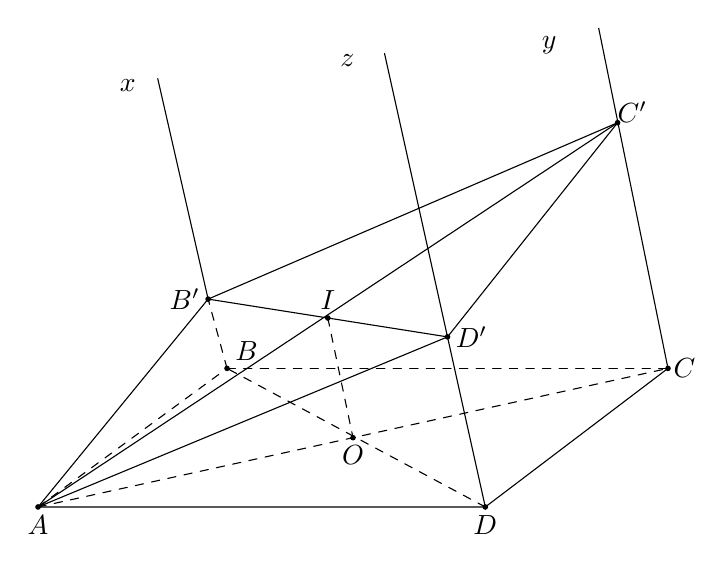
\begin{tikzpicture}[
			 x=1cm,y=1cm,xscale=1,yscale=-1,
		every node/.append style={scale=1},
		 inner sep=0pt,outer sep=0pt,
		dashstyle/.style={dashed,line cap=round}, 
		 solidstyle/.style={draw,line cap=round},scale=.8
		] 
	 \node at (3.5,5.4) [above right=3pt] {$B$};
	\node at  (0.5,7.6) [below=3pt] {$A$};
	\node at (8.5,0.4) [above right] {$y$}; 
	\node at (5.3,0.6)  [above right] {$z$};
	 \node at (1.8,1.0) [above right] {$x$};
	\node at (3.2,4.3)  [left=3pt] {$B'$};
	\node at (5.1,4.6) [above=3pt] {$I$}; 
	\node at (9.7,1.5)  [above right] {$C'$};
	\node at (7.0,4.9) [right=3pt]  {$D'$};
	\node  at (5.5,6.5) [below=3pt] {$O$};
	\node at  (10.5,5.4) [right=2pt] {$C$};
	 \node at (7.6,7.6) [below=3pt] {$D$};
	\draw[solid,fill] (3.5,5.4) circle  (1pt);
	\draw[solid,fill] (0.5,7.6) circle (1pt); 
	\draw[solid,fill] (3.2,4.3)  circle (1pt);
	 \draw[solid,fill] (5.1,4.6) circle (1pt);
	\draw[solid,fill] (9.7,1.5) circle (1pt); 
	\draw[solid,fill] (7.0,4.9) circle (1pt); 
	\draw[solid,fill] (5.5,6.5) circle (1pt); 
	\draw[solid,fill] (10.5,5.4) circle  (1pt);
	\draw[solid,fill] (7.6,7.6) circle (1pt); 
	\draw[dashstyle]  (5.1,4.6)--(5.5,6.5);
	\draw[solidstyle]  (3.2,4.3)--(7.0,4.9);
	\draw[solidstyle]  (0.5,7.6)--(9.7,1.5);
	\draw[solidstyle] (0.5,7.6)--(7.0,4.9)--(9.7,1.5)--(3.2,4.3)--cycle; 
	\draw[dashstyle] (7.6,7.6)--(3.5,5.4); 
	 \draw[dashstyle] (0.5,7.6)--(10.5,5.4);
	\draw[solidstyle]  (7.6,7.6)--(6.0,0.4);
	 \draw[solidstyle] (10.5,5.4)--(9.4,0.0);
	\draw[dashstyle]  (3.5,5.4)--(3.2,4.3);
	 \draw[solidstyle] (3.2,4.3)--(2.4,0.8);
	 \draw[solidstyle] (10.5,5.4)--(7.6,7.6)--(0.5,7.6);
	\draw[dashstyle] (0.5,7.6)--(3.5,5.4); 
	\draw[dashstyle]  (3.5,5.4)--(10.5,5.4);
\end{tikzpicture}
		} 
	 }
\end{ex}

% nguồn: Ok_Toan11_TracNghiem_Lan2
\begin{ex}%[1H4H2-2]%[ma:b0b4ee6c]
	Trong không gian, cho $3$ đường thẳng $ a$, $b$, $c$ chéo nhau từng đôi. Có nhiều nhất bao nhiêu đường  thẳng cắt cả $3$ đường thẳng ấy?
	 \choice
		{$1$} 
		{$2$} 
		 {$0$}
		{\True Vô số} 
	 \loigiai{
		Gọi $M$ là điểm bất kì nằm  trên $a$.\\
		Giả sử $d$ là đường thẳng qua $M$ cắt cả $b$ và $c$. Khi đó, $d$ là giao tuyến của mặt phẳng tạo  bởi $M$ và $b$ với mặt phẳng tạo bởi $M$ và $c$.\\
		Với mỗi điểm $M$  ta được một đường thẳng $d$.\\
	Vậy có  vô số đường thẳng cắt cả $3$ đường thẳng $a$, $b$, $c$.}
\end{ex}

% nguồn: Ok_Toan11_TracNghiem_Lan2
\begin{ex}%[1H4H2-2]%[ma:3e1df4c9]
	Cho hình chóp $S.ABCD$ có đáy $ABCD$ là hình chữ nhật. Gọi $M$, $N$ lần lượt là trung điểm của $AB$, $CD$ và $G_1$, $G_2$ lần lượt là trọng tâm của các cạnh tam giác $SAB$, $SCD$. Trong  các đường thẳng sau đây, đường thẳng nào không song song với $G_1G_2$?
	 \choice
		 {$AD$}
		 {$BC$}
		{\True  $SA$}
		 {$MN$}
	\loigiai{\immini{ 
		Gọi $M$, $N$ lần lượt là trung điểm của $AB$, $CD$ và $G_1$, $G_2$ lần lượt là trọng tâm  của các tam giác $SAB$, $SCD$ nên $G_1\in SM$, $G_2\in SN$.\\
		Và $\dfrac{S{G_1}}{SM}=\dfrac{S{G_2}}{SN}=\dfrac{1}{3}\Rightarrow{G_1}{G_2}\parallel MN\left(\parallel AD\parallel BC\right)$.}{\begin{tikzpicture}[scale=0.8,line cap=round,line join=round,>=stealth,font=\footnotesize]
		\def\a{4} 
		 \path (0:0) coordinate (A)
			++(0:\a)  coordinate (D)
			++(-130:\a/2)  coordinate (C)
			($(A)+(C)-(D)$)  coordinate (B)
			($(A)+(100:\a)$)  coordinate (S)
			($(A)!0.5!(B)$) coordinate  (M)
			 ($(C)!0.5!(D)$) coordinate (N)
			($(S)!2/3!(M)$) coordinate  (G_1)
			($(S)!2/3!(N)$) coordinate  (G_2)
			(intersection of A--C and B--D)  coordinate (O);
		\draw[dashed]  (B)--(A)--(D)
			 (A)--(S)--(M)--(N)
			(G_1)--(G_2); 
		\draw  (B)-- (C)--(D)
			 (B)--(S)
			(C)--(S)--(N) 
			 (D)--(S);
		\foreach \x/\g in  {A/135,B/-135,C/-45,D/45,S/90,G_1/35,G_2/20,M/-180,N/-20}
		 \fill (\x) circle (1pt)
			($(\g:3mm)+(\x)$) node {$\x$}; 
	\end{tikzpicture}
	 }}
\end{ex}

% nguồn: Ok_Toan11_TracNghiem_Lan2
\begin{ex}%[1H4H2-2]%[ma:76d95956]
	Cho hình chóp $S.ABC$ và $G$, $K$ lần  lượt là trọng tâm tam giác $SAB$, $SBC$. Khẳng định nào sau đây là đúng?
	 \choice
		{$GK\parallel  AB$}
		{$GK\parallel  BC$}
		{\True $GK\parallel  AC$}
		{$GK\parallel  SB$}
	 \loigiai{\immini{
		Gọi $M$,  $N$ lần lượt là trung điểm của $AB$, $BC$. Khi đó\\
		$\dfrac{SG}{SM}=\dfrac{2}{3}$ và  $\dfrac{SK}{SN}=\dfrac{2}{3}$ suy ra $\dfrac{SG}{SM}=\dfrac{SK}{SN}$.\\
		Suy ra $GK\,\parallel MN$ mà $MN \parallel  AC$.\\
		Nên $GK\parallel AC$.}{\begin{tikzpicture}[scale=0.8,line cap=round,line join=round,>=stealth,font=\footnotesize]
		 \def\a{4}
		\def\h{4} 
		\path (0:0) coordinate  (A)
			++(0:\a) coordinate (B) 
			++(-150:4*\a/5) coordinate (C) 
			($(A)+(60:\h)$)  coordinate (S)
			($(A)!0.5!(B)$) coordinate  (M)
			($(B)!0.5!(C)$) coordinate  (N)
			($(S)!2/3!(M)$)  coordinate (G)
			($(S)!2/3!(N)$) coordinate (K); 
		\draw  (A)--(C)--(B)
			 (A)--(S)
			(B)--(S)--(N) 
			 (C)--(S);
		\draw[dashed]  (S)--(M)
			 (A)--(B)
			 (G)--(K)
			 (M)--(N);
		 \foreach \x /\goc in {A/180,B/0,C/-135,S/90,M/40,N/-90,G/40,K/0}
		\fill (\x) circle  (1pt)
			 ($(\x)+(\goc:3mm)$) node {$\x$};
	\end{tikzpicture}
	} } 
\end{ex}

% nguồn: Ok_Toan11_TracNghiem_Lan2
\begin{ex}%[1H4H2-2]%[ma:a20a6404]
	Cho hình chóp $S.ABCD$ có $AD$ không song  song với $BC$. Gọi $M$, $N$, $P$, $Q$, $R$, $T$ lần lượt là trung điểm $AC$, $BD$, $BC$, $CD$, $SA$, $SD$. Cặp đường thẳng nào sau đây song song với nhau?
	 \choice
		{$MP$ và  $RT$}
		{\True $MQ$ và $RT$} 
		{$MN$ và  $RT$}
		{$PQ$  và $RT$}
	\loigiai{ 
	 \immini{
		Ta có $M$, $Q$  lần lượt là trung điểm của $AC$, $CD$.\\
		 $\Rightarrow MQ$ là đường trung bình của tam giác $CAD$.\\
		$\Rightarrow MQ\parallel AD$. $(1)$\\ 
		Ta có $R$, $T$ lần  lượt là trung điểm của $SA$, $SD$.\\
		$\Rightarrow RT$ là đường trung bình  của tam giác $SAD$.\\
		 $\Rightarrow RT\parallel AD$. $(2)$\\
		Từ $(1)$, $(2)$ suy ra $MQ\parallel RT$.}{\begin{tikzpicture}[scale=2,font=\footnotesize,line join=round,line cap=round,>=stealth]
		\coordinate (A) at  (0,1.6);
		\coordinate (B) at  (0.7,0.3);
		\coordinate (C)  at (2,0.6);
		\coordinate (D)  at (2.5,1.6);
		\coordinate (S) at (1,3); 
		\coordinate (R) at ($(S)!0.5!(A)$); 
		\coordinate (T) at ($(S)!0.5!(D)$); 
		\coordinate (P) at ($(B)!0.5!(C)$); 
		\coordinate (Q) at ($(C)!0.5!(D)$); 
		\coordinate (M) at ($(A)!0.5!(C)$); 
		\coordinate (N)  at ($(B)!0.5!(D)$);
		\draw (A) -- (B) -- (C) --  (D);
		 \draw [dashed] (A) -- (D);
		\draw [dashed]  (R) -- (T);
		\draw [dashed]  (P) -- (Q);
		\draw [dashed] (B) -- (D); 
		\draw [dashed] (A) --  (C);
		\draw [dashed]  (M) -- (N);
		\draw [dashed]  (M) -- (P);
		\draw [dashed] (M) -- (Q); 
		\draw (S) --  (A);
		 \draw (S) -- (B);
		 \draw (S) -- (C);
		\draw  (S) -- (D);
		\filldraw (R) circle (0.5pt) node[left]  {$R$};
		 \filldraw (T) circle (0.5pt) node[right] {$T$};
		\filldraw (P) circle (0.5pt) node[below]  {$P$};
		\filldraw  (Q) circle (0.5pt) node[right] {$Q$};
		\filldraw (M) circle  (0.5pt) node[above right] {$M$};
		 \filldraw (N) circle (0.5pt) node[below right] {$N$};
		\filldraw  (A) circle (0.5pt) node[above left] {$A$};
		\filldraw  (B) circle (0.5pt) node[below left] {$B$};
		\filldraw (C) circle (0.5pt) node[below  right] {$C$};
		\filldraw (D)  circle (0.5pt) node[above right] {$D$};
		\filldraw (S) circle (0.5pt) node[above]  {$S$};
	\end{tikzpicture}
	}} 
\end{ex}

% nguồn: Ok_Toan11_TracNghiem_Lan2
\begin{ex}%[1H4H2-2]%[ma:5978af5d]
	Cho hình chóp $S.ABCD$. Gọi $A'$, $B'$, $C'$, $D'$ lần lượt là trung điểm của các cạnh $SA$, $SB$, $SC$, $SD$. Trong các đường thẳng sau đây, đường thẳng nào  không song song với $A'B'$?
	 \choice
		 {$AB$}
		{$CD$} 
		 {$C'D'$}
		{\True $SC$} 
	\loigiai{ 
	\immini{Do $A'B'$ và $SC$ không đồng  phẳng nên $A'B'$ và $SC$ không song song nhau.}{
		\begin{tikzpicture}[scale=.6]
				\coordinate [label=left:$A$](A)  at (3,3);
				\coordinate  [label=below:$B$](B) at (0,0);
				\coordinate [label=below:$C$](C) at  (8,0);
				\coordinate [label=above:$S$](S) at (1.5,8); 
				\coordinate[label=right:$D$] (D) at  ($(C)-(B)+(A)$);
				\coordinate [label=above  left:$A'$](A') at ($(S)!.5 ! (A)$);
				\coordinate [label=left:$B'$](B') at ($(S)!.5  ! (B)$);
				\coordinate [label=right:$C'$](C')  at ($(S)!.5 ! (C)$);
				 \coordinate [label=above right:$D'$](D') at ($(S)!.5 ! (D)$);
				\foreach \diem in {A,B,C,D,S,A',B',C',D'} \fill (\diem) circle (1pt); 
				\draw[smooth](B)--(C) 
					(C)--(D) 
					(S)--(B) 
					(S)--(C) 
					(S)--(D) 
					 (B')--(C')--(D');
				\draw[dashed](A)--(S) 
					 (A)--(B)
					 (A)--(D)
					(B')--(A')--(D'); 
			\end{tikzpicture}
		 }
	 }
\end{ex}

% nguồn: Ok_Toan11_TracNghiem_Lan2
\begin{ex}%[1H4H2-2]%[ma:e828519e]
	Cho tứ diện $ABCD$. Gọi $G$ và $E$ lần lượt là trọng tâm của tam giác $ABD$ và $ABC$. Mệnh đề  nào dưới đây đúng ?
	\choice 
		{\True  $GE\parallel CD$}
		 {$GE$ cắt $AD$}
		{$GE$ cắt $CD$} 
		{$GE$  và $CD$ chéo nhau}
	 \loigiai{
	\immini{Ta có $\dfrac{AG}{AI}=\dfrac{AE}{AJ}=\dfrac{2}{3}$ nên $EG\parallel IJ$ mà $IJ\parallel CD\Rightarrow EG\parallel CD$.}{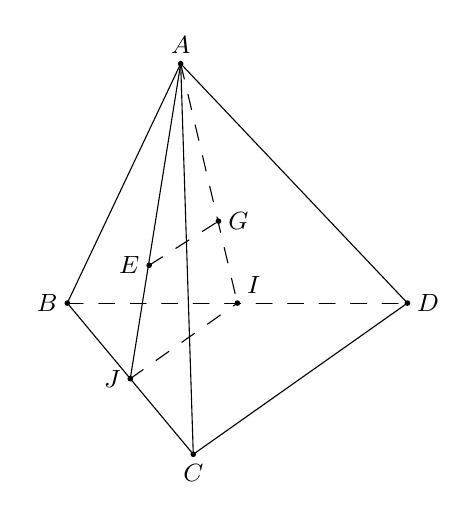
\begin{tikzpicture}[scale=.8,
			 x=1cm,y=1cm,xscale=1,yscale=-1,
			solid/.style={draw,line cap=round}, 
			 dashed/.style={solid,dash pattern=on 0.2cm off 0.2cm},
			every  node/.style={scale=1,font=\small}
			] 
		\coordinate (A)  at (6.1,0.5);
		\coordinate (B) at  (4.3,4.3);
		\coordinate (C)  at (6.3,6.7);
		\coordinate (D) at  (9.7,4.3);
		\coordinate  (E) at (7.0,4.3);
		 \coordinate (F) at (5.3,5.5);
		 \coordinate (G) at (5.6,3.7);
		 \coordinate (H) at (6.7,3.0);
		 \draw[solid] (D) -- (C);
		 \draw[solid] (B) -- (C);
		 \draw[solid] (B) -- (A)--(C);
		 \draw[solid] (A) -- (D);
		\draw[solid] (F)  -- (A);
		\draw[dashed] (B) -- (D); 
		\draw[dashed] (F) --  (E);
		\draw[dashed] (A)  -- (E);
		\draw[dashed] (G) -- (H); 
		 \draw[solid,fill] (A) circle (1pt) node[above] {$A$};
		 \draw[solid,fill] (B) circle (1pt) node[left] {$B$};
		\draw[solid,fill] (C) circle  (1pt) node[below] {$C$};
		\draw[solid,fill]  (D) circle (1pt) node[right] {$D$};
		\draw[solid,fill] (E) circle  (1pt) node[above right] {$I$};
		\draw[solid,fill] (F) circle (1pt)  node[left] {$J$};
		\draw[solid,fill] (G) circle (1pt) node[left] {$E$}; 
		 \draw[solid,fill] (H) circle (1pt) node[right] {$G$};
	\end{tikzpicture}
		 }
	} 
\end{ex}

% nguồn: Ok_Toan11_TracNghiem_Lan2
\begin{ex}%[1H4H2-2]%[ma:20167ebc]
	Cho tứ diện $ABCD$, gọi $I$ và $J$ lần lượt là trọng tâm của tam giác $ABD$ và $ABC$. Đường thẳng  $IJ$ song song với đường nào?
	 \choice
		 {$AB$}
		{\True  $CD$}
		{$BC$} 
		 {$AD$}
	\loigiai{ 
	\immini{ 
		Gọi $N$, $M$ lần lượt là trung điểm  của $BC$, $BD$.\\
		Do đó $MN$ là đường trung bình của tam giác $BCD$ nên  $MN\parallel CD$. $(1)$\\
		Vì $J$, $I$ lần lượt là trọng tâm các tam giác $ABC$  và $ABD$.\\ Suy ra $\dfrac{AI}{AM}=\dfrac{AJ}{AN}=\dfrac{2}{3}\Rightarrow IJ\parallel MN$. $(2)$\\
		Từ $(1)$ và $(2)$ suy ra $IJ\parallel CD$.}{\begin{tikzpicture}[scale=2,font=\footnotesize,line join=round,line cap=round,>=stealth]
		\coordinate (B) at  (0,1);
		 \coordinate (C) at (2,1);
		 \coordinate (D) at (1,0);
		 \coordinate (A) at (1.2,2.3);
		\coordinate (N)  at ($(B)!0.5!(D)$);
		\coordinate  (M) at ($(B)!0.5!(C)$);
		\coordinate  (I) at ($(A)!0.75!(M)$);
		 \coordinate (J) at ($(A)!0.6667!(N)$);
		\draw [dashed] (B) -- (C) -- (D); 
		 \draw (B) -- (D) -- (C);
		\draw (A) -- (B); 
		\draw (A) -- (C); 
		\draw (A) -- (D); 
		\filldraw  (N) circle (0.5pt) node[left] {$N$};
		\filldraw (M) circle (0.5pt)  node[below] {$M$};
		\draw  [dashed](M) -- (N);
		\draw [dashed](I)  -- (J);
		\draw [dashed](A) -- (M); 
		\draw (A)  -- (N);
		\filldraw (I) circle (0.5pt) node[right] {$I$}; 
		\filldraw (J) circle (0.5pt) node[left]  {$J$};
		\node at (A) [above right] {$A$}; 
		\node at  (B) [left] {$B$};
		\node at (C)  [right] {$C$};
		\node  at (D) [below] {$D$};
	\end{tikzpicture}
	}} 
\end{ex}

% nguồn: Ok_Toan11_TracNghiem_Lan2
\begin{ex}%[1H4H2-2]%[ma:b07344a3]
	 Cho tứ diện $ABCD.$ Gọi $M$, $N$, $P$, $Q$, $R$, $S$ theo thứ tự là trung điểm của các cạnh $AC$, $BD$, $AB$, $CD$, $AD$, $BC$. Bốn điểm nào sau đây không đồng phẳng?
	\choice 
		{$P$, $Q$, $R$,  $S$}
		{$M$, $P$,  $R$, $S$}
		{\True $M$,  $R$, $S$, $N$}
		{$M$,  $N$, $P$, $Q$}
	\loigiai{ 
		\begin{center}
			\begin{tikzpicture}[scale=1,font=\footnotesize,line join=round,line cap=round]
					\foreach \x\y\t in  {0/0/B,1.3/-1.6/D,4.5/0/C,1/3.5/A}
					\coordinate (\t)  at (\x,\y);
					\coordinate (M) at  ($(A)!1/2!(C)$);
					\coordinate  (N) at ($(B)!1/2!(D)$);
					\coordinate  (R) at ($(A)!1/2!(D)$);
					\coordinate (P) at ($(A)!1/2!(B)$); 
					\coordinate  (S) at ($(B)!1/2!(C)$);
					\coordinate  (Q) at ($(D)!1/2!(C)$);
					\draw (A)--(B)--(D)--(A)--(C)--(D) 
						 (R)--(P)--(N)--(R)--(M)--(Q)--(R);
					 \draw[dashed](B)--(C)
						(S)--(N)--(Q)--(S)--(M)--(P)--(S); 
					 \foreach \t/\g in {A/90,B/180,D/-90,C/0,M/50,R/190,P/150,Q/-90,N/-150,S/-120}
					\draw[fill=black] (\t) circle (1.0pt) 
						node[shift={(\g:9pt)}]{$\t$}; 
				\end{tikzpicture}
		\end{center}
		 Theo tính chất của đường trung bình của tam giác ta có\\
		$PS \parallel AC \parallel QR$ suy ra $P$,  $Q$, $R$, $S$ đồng phẳng.\\
		Tương tự, ta có được $PM \parallel BC \parallel NQ$ suy ra $P$, $M$,  $N$, $Q$ đồng phẳng.\\
		Và $NR \parallel CD \parallel SN$ suy ra $M$,  $R$, $S$, $N$ đồng phẳng.
	} 
\end{ex}

% nguồn: Ok_Toan11_TracNghiem_Lan2
\begin{ex}%[1H4H2-2]%[ma:3682710c]
	Cho tứ diện $ABCD$. Gọi $I$, $J$  lần lượt là trọng tâm các tam giác $ABC$ và $ABD$. Chọn khẳng định đúng trong các khẳng định sau?
	\choice 
		{\True $IJ$ song song  với $CD$}
		{$IJ$ song song với  $AB$}
		{$IJ$  chéo $CD$}
		 {$IJ$ cắt$AB$}
	\loigiai{ 
	\immini{Gọi $M$, $N$ lần lượt là trung  điểm của $BC$ và $BD$.\\
		Suy ra $MN$ là đường trung bình của tam giác $BCD$.\\ $\Rightarrow MN\parallel CD$. $(1)$\\ 
		$I$, $J$ lần lượt là trọng tâm các tam  giác $ABC$ và $ABD$.\\ $\Rightarrow\dfrac{AI}{AM}=\dfrac{AJ}{AN}=\dfrac{2}{3}\Rightarrow IJ\parallel MN$. $(2)$\\
		Từ $(1)$ và $(2)$ suy ra $IJ\parallel CD$. }{\begin{tikzpicture}[scale=2,font=\footnotesize,line join=round,line cap=round,>=stealth]
		\coordinate (B) at (0,1); 
		\coordinate  (C) at (2,1);
		\coordinate (D) at (1,0); 
		\coordinate  (A) at (1.2,2.3);
		\coordinate (N) at ($(B)!0.5!(D)$); 
		\coordinate  (M) at ($(B)!0.5!(C)$);
		\coordinate  (I) at ($(A)!0.75!(M)$);
		\coordinate  (J) at ($(A)!0.6667!(N)$);
		\draw [dashed]  (B) -- (C) -- (D);
		\draw (B) -- (D) --  (C);
		\draw (A) -- (B); 
		\draw (A)  -- (C);
		\draw (A) --  (D);
		\filldraw (N) circle (0.5pt) node[left]  {$N$};
		 \filldraw (M) circle (0.5pt) node[below] {$M$};
		\draw [dashed](M)  -- (N);
		\draw [dashed](I) -- (J); 
		 \draw [dashed](A) -- (M);
		\draw (A) -- (N); 
		\filldraw (I) circle (0.5pt) node[right] {$I$}; 
		\filldraw (J)  circle (0.5pt) node[left] {$J$};
		\node at  (A) [above right] {$A$};
		\node  at (B) [left] {$B$};
		\node at (C)  [right] {$C$};
		\node at (D) [below]  {$D$};
	\end{tikzpicture}
	}} 
\end{ex}

% nguồn: Ok_Toan11_TracNghiem_Lan2
\begin{ex}%[1H4H2-2]%[ma:5e80babf]
	Cho tứ diện $ABCD$. Trên các cạnh $AB$, $AD$ lần lượt lấy các điểm $M$, $N$ sao cho $\dfrac{AM}{AB}=\dfrac{AN}{AD}=\dfrac{1}{3}$. Gọi $P$, $Q$ lần lượt là trung điểm các cạnh $CD$, $CB$. Mệnh đề nào  sau đây đúng?
	\choice 
		 {\True Tứ giác $MNPQ$ là một hình thang}
		 {Tứ giác $MNPQ$ là hình bình hành}
		{Bốn điểm $M$, $N$, $P$, $Q$ không  đồng phẳng}
		{Tứ giác $MNPQ$ không có  các cặp cạnh đối nào song song}
	 \loigiai{
	\immini{Xét  tam giác $ABD$ có $\dfrac{AM}{AB}=\dfrac{AN}{AD}=\dfrac{1}{3}$ nên $ MN\parallel BD$.\\
		 Xét tam giác $BCD$ có $PQ$ là đường trung bình của tam giác $ PQ\parallel BD$.\\
		Vậy $PQ\parallel MN$ nên $MNPQ$  là hình thang.}
		{ 
		\begin{tikzpicture}[scale=.6,font=\footnotesize,line join=round,line cap=round,>=stealth]
				\coordinate [label=left:$C$](C)  at (0,0);
				\coordinate [label=above:$D$](D) at (2,7); 
				\coordinate  [label=below:$B$](B) at (4,-3);
				\coordinate [label=right:$A$](A)  at (9,2);
				\coordinate[label=below:$M$] (M) at ($(A)! 1/3 !  (B)$);
				\coordinate[label=below:$Q$] (Q) at ($(B)!.5 !  (C)$);
				 \coordinate[label=above left:$P$] (P) at ($(C)!.5 ! (D)$);
				\coordinate[label=above right:$N$] (N) at ($(A)!  1/3 ! (D)$);
				\foreach \diem in  {A,B,C,D,M,N,P,Q} \fill (\diem) circle (1pt);
				\draw[smooth](D)--(A)--(B)--(C)--(D)--(B) 
					 (Q)--(P)
					 (N)--(M);
				 \draw[dashed](A)--(C)
					(Q)--(M) 
					(P)--(N); 
			\end{tikzpicture}
		 }
	} 
\end{ex}

% nguồn: Ok_Toan11_TracNghiem_Lan2
\begin{ex}%[1H4H2-2]%[ma:862bb2f9]
	Cho tứ diện $ABCD$. Gọi $M$, $N$ là hai điểm  phân biệt cùng thuộc đường thẳng $AB$; $P$, $Q$ là hai điểm phân biệt cùng thuộc đường thẳng $CD$. Xác định vị trí tương đối của $MQ$ và $NP$.
	 \choice
		{$MQ$ cắt  $NP$}
		{$MQ\parallel  NP$}
		{$MQ\equiv NP$} 
		 {\True $MQ$, $NP$ chéo nhau}
	\loigiai{ 
	\immini{ 
		Xét mặt phẳng $\left(ABP\right)$. Ta  có $M$, $N$ thuộc $AB$ nên $M$, $N$ thuộc mặt phẳng $\left(ABP\right)$.\\
		 Mặt khác $CD\cap\left(ABP\right)=P$.\\
		Mà $Q\in CD\Rightarrow Q\notin\left(ABP\right)$$\Rightarrow M$, $N$, $P$, $Q$ không đồng phẳng $\Rightarrow MQ$ và $ NP$ chéo nhau.}{\begin{tikzpicture}[scale=2,font=\footnotesize,line join=round,line cap=round,>=stealth]
		\coordinate (B) at  (0,1);
		\coordinate (D)  at (3,1);
		\coordinate (C) at (1.5,0); 
		\coordinate (A) at (1.5,3); 
		\draw (B) --  (C)--(D);
		\draw [dashed](B) --  (D);
		\draw (A) --  (B);
		\draw (A)  -- (C);
		\draw (A) -- (D); 
		 \coordinate (M) at ($(A)!0.3!(B)$);
		\coordinate (N)  at ($(A)!0.7!(B)$);
		\coordinate (P) at ($(C)!0.4!(D)$); 
		\coordinate (Q) at  ($(C)!0.75!(D)$);
		\filldraw (M) circle (0.5pt) node[left]  {$M$};
		\filldraw (N) circle  (0.5pt) node[left] {$N$};
		\filldraw (P) circle  (0.5pt) node[below right] {$P$};
		\filldraw  (Q) circle (0.5pt) node[below right] {$Q$};
		\draw [dashed](M) --  (P);
		 \draw [dashed](N) -- (Q);
		\draw [dashed](B) --  (P);
		\node at (A) [above]  {$A$};
		\node  at (B) [left] {$B$};
		\node at (C) [below]  {$C$};
		\node at  (D) [right] {$D$};
	\end{tikzpicture}
	}} 
\end{ex}

% nguồn: Ok_Toan11_TracNghiem_Lan2
\begin{ex}%[1H4H2-2]%[ma:83692064]
	Cho hình chóp $S.ABCD$ có đáy $ABCD$ là hình bình hành  tâm $O$. Gọi $I$, $J$ lần lượt là trung điểm của $SA$ và $SC$. Đường thẳng $IJ$ song song với đường thẳng nào?
	\choice 
		{$BC$} 
		{\True $AC$} 
		 {$SO$}
		 {$BD$}
	\loigiai{ 
	\immini{Dễ  dàng thấy được $IJ$ là đường trung bình của tam giác $SAC$.\\
		Nên  $IJ\parallel AC$.}{
		\begin{tikzpicture}[scale=1.5,font=\footnotesize,line join=round,line cap=round,>=stealth]
				\coordinate (A) at (0,0); 
				\coordinate (B)  at (2,0);
				\coordinate (C) at (3,1.5); 
				\coordinate (D) at  (1,1.5);
				 \coordinate (O) at ($(A)!0.5!(C)$);
				\coordinate  (S) at ($(O)+(0,2.5)$);
				 \coordinate (I) at ($(S)!0.5!(A)$);
				 \coordinate (J) at ($(S)!0.5!(C)$);
				\draw (A) -- (B) --  (C);
				\draw [dashed](A) -- (D) -- (C); 
				\draw  (S) -- (A);
				 \draw (S) -- (B);
				\draw  (S) -- (C);
				\draw  [dashed](S) -- (D);
				 \draw[dashed] (A) -- (C);
				\draw[dashed] (B)  -- (D);
				\draw[dashed]  (S) -- (O);
				\draw[dashed] (I) -- (J); 
				\node at (A)  [below left] {$A$};
				\node at  (B) [below right] {$B$};
				\node at (C) [above right]  {$C$};
				 \node at (D) [below] {$D$};
				\node at (O)  [below] {$O$};
				\node at (S) [above]  {$S$};
				\node at (I) [left]  {$I$};
				 \node at (J) [right] {$J$};
				\filldraw[black] (I) circle  (0.5pt);
				\filldraw[black] (J) circle (0.5pt); 
			\end{tikzpicture}
		} 
	 }
\end{ex}

% nguồn: Ok_TracNghiemLop11_Lan1
\begin{ex}%[1H4H2-2]%[ma:3b9859ce]
	Cho hình chóp tứ giác $S.ABCD$. Gọi $G_1$, $G_2$ lần lượt là trọng tâm các tam giác $SAC$  và $ACD$. Khi đó $G_1G_2$ song song với đường thẳng
	 \choice
		{$AC$} 
		 {$AD$}
		{\True  $SD$}
		{$BC$} 
	 \loigiai{
	\immini{ 
		Gọi  $E$ là trung điểm của $AC$. \\
		Trong $\triangle  SED$, ta có $$\dfrac{EG_1}{ES}=\dfrac{EG_2}{ED}=\dfrac{1}{3}.$$
		Suy ra $G_1G_2\parallel SD$. 
		}{\begin{tikzpicture}[line join=round,line cap=round,>=stealth,scale=0.7,font=\footnotesize]
		\foreach \x/\y/\n in {0/0/A,1/-2.5/D,4.5/-2/C,6/0/B} \coordinate (\n) at (\x,\y); 
		\coordinate (S) at  ($(A)+(2,4)$);
		\coordinate (E)  at ($(C)!0.5!(A)$);
		\coordinate (G_1) at ($(S)!2/3!(E)$); 
		\coordinate  (G_2) at ($(D)!2/3!(E)$);
		\draw (S)--(A)--(D)--(C)--(B)--(S)--(C) 
			 (S)--(D);
		\draw[dashed] (C)--(A)--(B) 
			(S)--(E)--(D) 
			(G_1)--(G_2); 
		 \foreach \t/\g in {A/180,B/0,C/-30,D/-150,S/90,E/30,G_1/0,G_2/-45}{
			\draw[fill] (\t)  circle (1pt) node[shift={(\g:8pt)}]{$ \t $};
		} 
	\end{tikzpicture}
		} 
	} 
\end{ex}

% nguồn: Ok_TracNghiemLop11_Lan1
\begin{ex}%[1H4H2-2]%[ma:c6f235cf]
	Cho  tứ diện $ABCD$. Gọi $I$, $J$ lần lượt là trọng tâm của tam giác $ABC$, $ABD$. Tìm khẳng định đúng trong các khẳng định sau đây.
	\choice 
		{Hai đường thẳng $IJ$ và  $CD$ cắt nhau}
		{Hai đường thẳng $IJ$ và $CD$ chéo  nhau}
		{\True Hai đường thẳng $IJ$ và $CD$  song song nhau và $IJ=\dfrac{1}{3}CD$}
		{Hai đường thẳng $IJ$ và $CD$ song song  nhau và $IJ=\dfrac{2}{3}CD$}
	 \loigiai{
	\immini{ 
		Gọi $E$ là  trung điểm của $AB$.\\
		Vì $I$, $J$ là trọng tâm của tam giác $ABC$, $ABD$ nên  $$\dfrac{EI}{EC}=\dfrac{EJ}{ED}=\dfrac{1}{3}\Rightarrow IJ\parallel CD \text{ và }IJ=\dfrac{1}{3}CD.$$
		}{\begin{tikzpicture}[line join=round,line cap=round,>=stealth,scale=0.6,font=\footnotesize]
		\foreach \x/\y/\n in {0/0/B,2/-2/C,6/0/D} \coordinate (\n) at (\x,\y); 
		\coordinate (A) at  ($(B)+(2,4)$);
		\coordinate (E) at ($(B)!0.5!(A)$); 
		\coordinate (I) at  ($(C)!2/3!(E)$);
		\coordinate (J) at  ($(D)!2/3!(E)$);
		\draw (A)--(B)--(C)--(D)--(A)--(C)--(E); 
		\draw[dashed]  (B)--(D)
			(D)--(E) 
			(I)--(J); 
		\foreach \t/\g in {A/90,B/180,C/-90,D/0,I/180,J/60,E/160}{ 
			\draw[fill]  (\t) circle (1pt) node[shift={(\g:8pt)}]{$ \t $};
		 }
	\end{tikzpicture}
		} 
	} 
\end{ex}

% nguồn: Ok_TracNghiemLop11_Lan1
\begin{ex}%[1H4H2-2]%[ma:95bfe17f]
	Cho hình chóp $S.ABCD$. Gọi $M$, $N$, $P$, $Q$, $R$, $T$ lần lượt là trung điểm $AC$, $BD$, $BC$, $CD$, $SA$, $SD$. Cặp đường thẳng nào sau đây  song song với nhau?
	\choice 
		 {$MP$ và $RT$}
		{\True $MQ$ và $RT$} 
		 {$MN$ và $RT$}
		{$PQ$  và $RT$}
	 \loigiai{
	 \immini{
		 Ta có $RT$ là đường trung bình của $\triangle SAD$.\\
		Suy ra  $RT\parallel AD$.\quad (1)\\
		Lại có $MQ$ là đường trung  bình của $\triangle ACD$.\\
		 Suy ra $MQ\parallel AD$.\quad (2)\\
		Từ (1) và  (2) $\Rightarrow MQ\parallel RT$.
		}{\begin{tikzpicture}[line join=round,line cap=round,>=stealth,scale=0.7,font=\footnotesize]
		\foreach \x/\y/\n in {0/0/A,1/-2/D,3.5/-2.5/C,6/0/B}  \coordinate (\n) at (\x,\y);
		\coordinate  (S) at ($(A)+(2,4)$);
		\coordinate  (M) at ($(C)!0.5!(A)$);
		\coordinate (N) at ($(B)!0.5!(D)$); 
		 \coordinate (P) at ($(B)!0.5!(C)$);
		\coordinate  (Q) at ($(C)!0.5!(D)$);
		\coordinate (R) at ($(S)!0.5!(A)$); 
		 \coordinate (T) at ($(S)!0.5!(D)$);
		 \draw (S)--(A)--(D)--(C)--(B)--(S)--(C)
			 (S)--(D)
			(R)--(T); 
		\draw[dashed]  (C)--(A)--(B)--(D)
			 (M)--(Q);
		\foreach \t/\g in  {A/180,B/0,C/-30,D/-150,S/90,R/150,T/0,M/60,N/80,Q/-100,P/-20}{
			\draw[fill] (\t)  circle (1pt) node[shift={(\g:8pt)}]{$ \t $};
		 }
	\end{tikzpicture}
		} 
	} 
\end{ex}

% nguồn: Ok_TracNghiemLop11_Lan1
\begin{ex}%[1H4H2-2]%[ma:8413255f]
	Cho tứ diện $ABCD$. Gọi $M$, $N$, $P$, $Q$ lần lượt là trung điểm của  các cạnh $AB$, $AD$, $CD$, $BC$. Mệnh đề nào sau đây \textbf{sai}?
	\choice 
		 {$MN\parallel BD$}
		{$MQ\parallel NP$} 
		 {$MN=PQ$}
		{\True $4$  điểm $M$, $N$, $P$, $Q$ không đồng phẳng}
	 \loigiai{
	\immini{Ta có $MN$, $PQ$ lần lượt là đường trung bình tam giác $ABD$ và tam giác $BCD$ nên 
		$\left\{\begin{aligned}
		& MN\parallel BD,MN=\dfrac{1}{2}BD \\ 
		& PQ\parallel  BD,PQ=\dfrac{1}{2}BD. \\
	\end{aligned} \right.$ \\
	Suy ra $MN  \parallel PQ$, $MN=PQ$.\\
	Vậy $MNPQ$ là hình  bình hành.\\
	Vậy $MN\parallel BD$, $MQ\parallel NP$, $MN=PQ$  là trả lời đúng.\\
	Khẳng  định $4$ điểm $M$, $N$, $P$, $Q$ không đồng phẳng là trả lời sai.
	}{ 
	\begin{tikzpicture}[scale=0.8,font=\footnotesize,line join=round,line cap=round,>=stealth]
			\coordinate  (B) at (-2,0);
			\coordinate (C) at (-1,-2); 
			\coordinate  (D) at (3,0);
			\coordinate (A) at  ($(B)+(2,3)$);
			\coordinate (M)  at ($(B)!0.5!(A)$);
			 \coordinate (N) at ($(A)!0.5!(D)$);
			\coordinate  (P) at ($(D)!0.5!(C)$);
			\coordinate (Q) at ($(B)!0.5!(C)$); 
			 \draw (A)--(B)
				(A)--(C) 
				 (A)--(D)
				(C)--(D) 
				 (B)--(C)
				(M)--(Q) 
				(N)--(P); 
			\draw[dashed](B)--(D) 
				 (M)--(N)
				(Q)--(P); 
			\foreach \i/\g in {A/90,B/180,C/-90,D/0,M/180,N/0,P/-45,Q/180}{\draw[fill](\i)  circle (1pt)
				($(\i)+(\g:4mm)$)  node[scale=1]{$\i$};}
		\end{tikzpicture}
	 }
	 }
\end{ex}

% nguồn: Ok_TracNghiemLop11_Lan1
\begin{ex}%[1H4H2-2]%[ma:af5f902a]
	Cho hai đường thẳng chéo nhau $a$ và $b$. Lấy $A$, $B$ thuộc $a$ và $C$, $D$ thuộc $b$. Khẳng định nào sau đây đúng khi nói về hai đường thẳng $AD$ và  $BC$?
	 \choice
		{Có thể song song hoặc  cắt nhau}
		{Cắt  nhau}
		 {Song song nhau}
		{\True  Chéo nhau}
	 \loigiai{
		Ta có $a$ và $b$ chéo nhau nên $A$, $B$, $C$, $D$ không đồng phẳng.  Do đó $AD$ và $BC$ chéo nhau.
	 }
\end{ex}

% nguồn: Ok_TracNghiemLop11_Lan1
\begin{ex}%[1H4H2-2]%[ma:9432d044]
	Cho tứ diện $ABCD$. Gọi $I$, $J$ lần lượt là trọng tâm các tam giác $ABC$ và  $ABD$. Chọn khẳng định đúng trong các khẳng định sau.
	 \choice
		{\True  $IJ$ song song với $CD$}
		 {$IJ$ song song với $AB$}
		{$IJ$ chéo $CD$} 
		{$IJ$ cắt  $AB$}
	\loigiai{ 
	 \immini{
		Gọi $M$, $N$ lần lượt là trung điểm  của $BC$, $BD$.\\
		Ta có  $MN\parallel CD$.\\
		Xét $\triangle AMN$  có $\dfrac{AI}{AM}=\dfrac{AJ}{AN}=\dfrac{2}{3}\Rightarrow IJ\parallel MN$.\\
		 Suy ra $IJ\parallel CD$.
		}{\begin{tikzpicture}[line join=round,line cap=round,>=stealth,scale=0.6,font=\footnotesize]
		\foreach \x/\y/\n in {0/0/B,2/-2/C,6/0/D}  \coordinate (\n) at (\x,\y);
		\coordinate (A) at  ($(B)+(2,4)$);
		\coordinate (M)  at ($(B)!0.5!(C)$);
		 \coordinate (N) at ($(B)!0.5!(D)$);
		\coordinate (I)  at ($(A)!2/3!(M)$);
		\coordinate  (J) at ($(A)!2/3!(N)$);
		 \draw (A)--(B)--(C)--(D)--(A)--(C)
			 (A)--(M);
		\draw[dashed] (B)--(D) 
			 (M)--(N)--(A)
			 (I)--(J);
		\foreach \t/\g  in {A/90,B/180,C/-90,D/0,I/180,J/0,M/-150,N/45}{
			\draw[fill]  (\t) circle (1pt) node[shift={(\g:8pt)}]{$ \t $};
		 }
	\end{tikzpicture}
		 }
	 }
\end{ex}

% nguồn: Ok_TracNghiemLop11_Lan1
\begin{ex}%[1H4H2-2]%[ma:2d625fa5]
	Cho tứ diện $ABCD$, gọi các điểm $M$, $N$, $P$, $Q$ lần lượt là trung điểm các cạnh $AB$, $CD$, $AC$ và $BD$. Khi đó mệnh để nào  sau đây đúng?
	 \choice
		{$MN$, $PQ$, $BC$ đôi một  song song}
		{$MP\parallel BD$} 
		{$MN\parallel  PQ$}
		 {\True $MP\parallel NQ$}
	 \loigiai{
	\immini{ 
		Ta  có $MP$, $NQ$ lần lượt là đường trung bình của các tam giác $ABC$ và $BCD$ nên
		$$MP\parallel BC\text{ và }MQ\parallel BC\Rightarrow MP\parallel  NQ.$$
		}{\begin{tikzpicture}[line join=round,line cap=round,>=stealth,scale=0.5,font=\footnotesize]
		\foreach \x/\y/\n in {0/0/B,4/-2/C,6/0/D} \coordinate (\n) at  (\x,\y);
		\coordinate (A) at ($(B)+(3,4)$); 
		\coordinate (M) at ($(A)!1/2!(B)$); 
		\coordinate (P) at  ($(A)!1/2!(C)$);
		\coordinate (N)  at ($(C)!1/2!(D)$);
		\coordinate (Q) at  ($(B)!1/2!(D)$);
		\draw  (A)--(B)--(C)--(D)--(A)--(C)
			(M)--(P); 
		 \draw[dashed] (B)--(D)
			 (N)--(Q);
		\foreach  \t/\g in {A/90,B/180,C/-90,D/0,P/30,Q/-125,M/150,N/-20}{
			\draw[fill]  (\t) circle (1pt) node[shift={(\g:8pt)}]{$ \t $};
		} 
	\end{tikzpicture}
		} 
	 }
\end{ex}

% nguồn: Ok_TracNghiemLop11_Lan1
\begin{ex}%[1H4H2-2]%[ma:2b2d7335]
	Cho  tứ diện $ABCD$, $G$ là trọng tâm tứ diện. Gọi $G_1$ là giao điểm của $AG$ và mp$\left(BCD\right)$, $G_2$ là giao điểm của $BG$ và mp$\left(ACD\right)$. Khẳng định nào sau đây là đúng?
	 \choice
		{\True $G_1G_2 \parallel  AB$}
		{$G_1G_2\parallel  AC$}
		{$G_1G_2\parallel  CD$}
		{$G_1G_2\parallel  AD$}
	\loigiai{ 
	\immini{ 
		 Gọi $M$, $N$ lần lượt là trung điểm của $DC$, $AC$. \\
		Vì $G$ là trọng tâm tứ diện  nên $G$ là giao điểm của ba đoạn thẳng nối hai trung điểm của cặp cạnh đối của tứ diện.\\
		Xét  $\left(ABM\right)$ có $AG\cap BM=G_1$, $BG\cap AM=G_2$. \\
		Trong $\Delta ACD$ có $AM$ và $DN$  là đường trung tuyến nên $G_2$ là trọng tâm của tam giác do đó $\dfrac{G_2M}{G_2A}=\dfrac{1}{2}$.\\
		Tương tự ta cũng có $\dfrac{G_1M}{G_1B}=\dfrac{1}{2}$ suy ra $G_1G_2\parallel AB$ . 
		}{\begin{tikzpicture}[line join=round,line cap=round,>=stealth,scale=0.75,font=\footnotesize]
		\foreach \x/\y/\n  in {0/0/B,1.5/-1.5/C,6/0/D} \coordinate (\n) at (\x,\y);
		\coordinate  (A) at ($(B)+(3,5)$);
		\coordinate (M)  at ($(C)!1/2!(D)$);
		\coordinate (N) at  ($(A)!1/2!(C)$);
		 \coordinate (P) at ($(A)!1/2!(B)$);
		\coordinate (Q) at  ($(A)!1/2!(D)$);
		\coordinate (R) at  ($(B)!1/2!(C)$);
		 \coordinate (G) at ($(P)!1/2!(M)$);
		 \coordinate (G_1) at ($(B)!2/3!(M)$);
		 \coordinate (G_2) at ($(A)!2/3!(M)$);
		\draw  (A)--(B)--(C)--(D)--(A)--(C)
			 (A)--(M)
			 (D)--(N);
		\draw[dashed]  (B)--(D)
			(M)--(P) 
			(Q)--(R) 
			(A)--(G_1) 
			(B)--(M) 
			(B)--(G_2); 
		\foreach \t/\g in  {A/90,B/180,C/-90,D/0,P/120,Q/45,R/-150,M/-50,N/110,G_1/-90,G_2/30,G/-20}{
			\draw[fill] (\t) circle  (1pt) node[shift={(\g:8pt)}]{$ \t $};
		} 
	\end{tikzpicture}
		 }
	} 
\end{ex}

% nguồn: Ok_TracNghiemLop11_Lan1
\begin{ex}%[1H4H2-2]%[ma:c6b463cf]
	Cho hình chóp tứ giác $S.ABCD$ có đáy $ABCD$ là hình bình hành tâm $O$. Gọi $I$ là trung điểm của $SA$. Đường  thẳng $IO$ song song với đường thẳng nào?
	\choice 
		 {$SA$}
		 {\True $SC$}
		{$SD$} 
		{$SB$} 
	\loigiai{ 
	\immini{Vì $I$, $O$ lần lượt là trung điểm của $SA$, $AC$  nên $IO$ là đường trung bình của tam giác $SAC$. Suy ra $IO \parallel SC$.}
		{\begin{tikzpicture}[scale=.7]
		\def\a{4} 
		 \path (0:0) coordinate (A)
			 ++(0:\a) coordinate (D)
			++(-50:.55*\a) coordinate (C) 
			($(A)+(C)-(D)$)  coordinate (B)
			(intersection of  A--C and B--D) coordinate (O)
			($(O)+(70:\a)$) coordinate (S) 
			($(S)!.5!(A)$) coordinate (I); 
		\draw[dashed]  (A)--(D)--(C)
			(D)--(S) 
			(S)--(O) 
			(A)--(C) 
			(B)--(D) 
			 (O)--(I);
		\draw (A)-- (B)--(C) 
			(B)--(S) 
			 (C)--(S)
			 (A)--(S);
		 \foreach \x/\g in {A/180,B/-135,C/-45,D/0,S/90,O/-90,I/120}
		\fill[black]  (\x) circle (1pt)
			 ($(\g:3mm)+(\x)$) node {$\x$};
	\end{tikzpicture}
		 }
	 }
\end{ex}

% nguồn: Ok_TracNghiemLop11_Lan1
\begin{ex}%[1H4H2-2]%[ma:d531e706]
	\immini[thm]{Cho hình chóp  $S.ABCD$. Gọi $G$, $E$ lần lượt là trọng tâm các tam giác $SAD$ và $SCD$. Lấy $M$, $N$ lần lượt là trung điểm $AB$, $BC$. Khi đó ta có
	\choice 
		{$GE$ và $MN$ trùng  nhau}
		{$GE$ và  $MN$ chéo nhau}
		{\True $GE$ và $MN$  song song với nhau}
		 {$GE$ cắt $BC$}
		}{\begin{tikzpicture}[line join=round,line cap=round,>=stealth,scale=0.65,font=\footnotesize]
		 \tikzset{every node/.style={outer sep=-0.5mm}}
		\foreach \x/\y/\n in {0/0/A,1.5/-2/B,6/0/D,5/-1.5/C} \coordinate (\n) at  (\x,\y);
		\coordinate (O)  at (intersection of A--C and B--D);
		 \coordinate (S) at ($(A)+(3,4)$);
		\coordinate (M)  at ($(A)!0.5!(B)$);
		\coordinate (N)  at ($(C)!0.5!(B)$);
		\coordinate  (H) at ($(A)!0.5!(D)$);
		\coordinate (G) at  ($(S)!2/3!(H)$);
		\coordinate  (K) at ($(C)!0.5!(D)$);
		\coordinate (E) at ($(S)!2/3!(K)$); 
		\draw[thin,dashed] (A)--(D) 
			(S)--(H); 
		 \draw (B)--(A)--(S)--(B)--(C)--(D)--(S)--(C)
			(S)--(K); 
		\foreach \n/\l in {A/above left,B/below left,C/below right,D/above right,S/above,M/below left,N/below,G/left,E/right} \fill (\n) node[\l]{$\n$}  circle (1pt);
		\foreach \x/\y  in {A/D,C/D} \fill ($(\x)!1/2!(\y)$) circle (1pt);
	\end{tikzpicture}
		} 
	\loigiai{ 
	\immini{Gọi $I$ là trung điểm của $SD$. Xét tam giác  $IAC$ có $$\dfrac{IG}{IA}=\dfrac{IE}{IC}=\dfrac{1}{3}.$$
		Theo định lí đảo của định lí Thalet, ta có $GE\parallel AC$\quad (1).\\ 
		Mặt khác, ta có $MN$ là đường trung  bình của $\triangle ABC$ nên suy ra $MN\parallel AC$\quad (2).\\
		Từ (1) và (2)  ta có $MN\parallel GE$}
		{\begin{tikzpicture}[line join=round,line cap=round,>=stealth,scale=0.65,font=\footnotesize]
		\tikzset{every node/.style={outer sep=-0.5mm}} 
		\foreach \x/\y/\n in {0/0/A,1.5/-2/B,6/0/D,5/-1.5/C} \coordinate (\n)  at (\x,\y);
		\coordinate (O) at (intersection  of A--C and B--D);
		\coordinate  (S) at ($(A)+(3,4)$);
		 \coordinate (M) at ($(A)!0.5!(B)$);
		\coordinate (N) at ($(C)!0.5!(B)$); 
		\coordinate (H) at ($(A)!0.5!(D)$); 
		\coordinate (G) at ($(S)!2/3!(H)$); 
		\coordinate (K) at ($(C)!0.5!(D)$); 
		\coordinate (E) at  ($(S)!2/3!(K)$);
		 \coordinate (I) at ($(S)!1/2!(D)$);
		 \draw[thin,dashed] (A)--(D)
			 (S)--(H)
			(I)--(A) 
			 (G)--(E)
			 (A)--(C)
			(M)--(N); 
		\draw (B)--(A)--(S)--(B)--(C)--(D)--(S)--(C) 
			(S)--(K) 
			(I)--(C); 
		\foreach \n/\l in {A/above left,B/below left,C/below right,D/above right,S/above,M/below left,N/below,G/above left,E/right,I/above right} \fill (\n) node[\l]{$\n$}  circle (1pt);
		\foreach \x/\y in  {A/D,C/D} \fill ($(\x)!1/2!(\y)$) circle (1pt);
	\end{tikzpicture}
	 }}
\end{ex}

% nguồn: Ok_TracNghiemLop11_Lan1
\begin{ex}%[1H4V2-2]%[ma:c463a965]
	Cho hình chóp $S.ABCD$ có đáy là hình bình hành. Gọi $M,\, N$ lần lượt là trung điểm của $AB$ và $CD$, $P$ là điểm thuộc $SA$. Giao tuyến  của hai mặt phẳng $(SAD)$ và $(PMN)$ là đường thẳng:
	\choice 
		{Qua $P$ song song với $AB$} 
		{\True Qua $P$ song  song với $AD$}
		{$PD$} 
		{Qua $P$ song song với $MC$} 
	 \loigiai{
		\begin{center}
			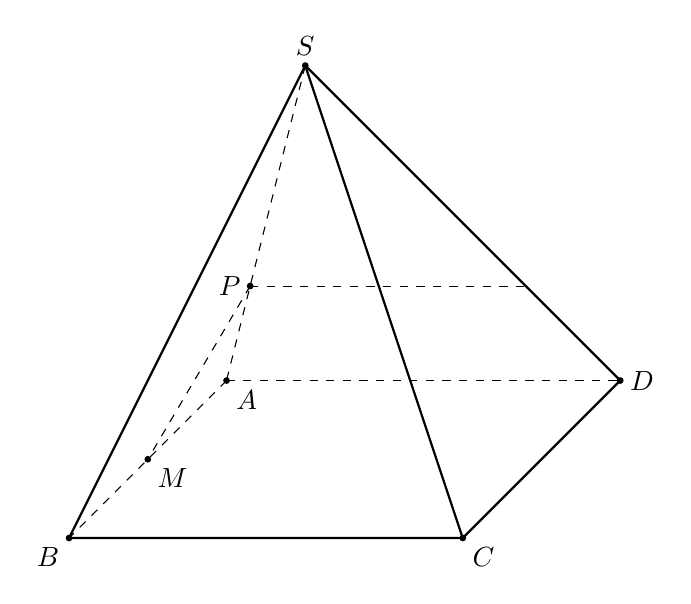
\begin{tikzpicture}
					\coordinate (A)  at (0,0);
					\coordinate (B) at (-2,-2); 
					\coordinate  (C) at (3,-2);
					\coordinate (D) at (5,0); 
					 \coordinate (S) at (1,4);
					\coordinate  (M) at (-1,-1);
					\coordinate (P)  at (0.3,1.2);
					 \coordinate (P1) at (3.8,1.2);
					\draw [thick] (B) -- (C) --  (D);
					\draw [thick] (S) --  (B);
					\draw [thick]  (S) -- (C);
					\draw [thick] (S)  -- (D);
					\draw [dashed] (S)  -- (A);
					 \draw [dashed] (A) -- (B);
					\draw [dashed] (A) --  (D);
					\draw  [dashed] (P) -- (P1);
					\draw [dashed]  (P) -- (M);
					\filldraw (S)  circle (1pt) node[above] {$S$};
					\filldraw (A)  circle (1pt) node[below right] {$A$};
					\filldraw (B)  circle (1pt) node[below left] {$B$};
					\filldraw  (C) circle (1pt) node[below right] {$C$};
					\filldraw (D) circle (1pt) node[right]  {$D$};
					\filldraw (M) circle (1pt) node[below right]  {$M$};
					\filldraw (P) circle  (1pt) node[left] {$P$};
				\end{tikzpicture}
		\end{center}
		Ta có: $\heva{&MN  \parallel AD\\&MC \subset (PMN)\\&AD \subset (SAD)\\&P \in (PMN) \cap (SAD)}$\\
		Nên giao  tuyến của hai mặt phẳng $(SAD)$ và $(PMN)$ là đường thẳng qua $P$ song song với $AD$.
	} 
\end{ex}


%%%%%%%%%%%%%%%% ĐÚNG/SAI %%%%%%%%%%%%%%%%

% nguồn: Ok_dungsai_lop11_Lan1
\begin{ex}%[1H4N2-2]%[ma:6e6d8875]
 Cho hình chóp $S.ABCD$ có đáy là hình thang với đáy lớn $AD=2BC$. Gọi $I$  là giao điểm của $AC$ và $BD$, $G$ là trọng tâm của $\triangle SCD$.
  \choiceTF
  {\True Hai đường thẳng $SA$ và $BD$  chéo nhau}
  {Hai đường thẳng $SA$ và $IG$ song song với  nhau}
  {\True Trên cạnh $SA$ lấy điểm  $K$ sao cho $SK=\dfrac{1}{2}KA$. Khi đó $IK$ song song với $SC$ }
  {\True Điểm $M$ là trung điểm của $SC$,  khi đó $BM$ song song với $IG$}
 \loigiai{ 
  \begin{tikzpicture}[>=stealth,line join=round,line cap = round,scale=1,font=\footnotesize]
     \def\ad{6}
    \def\ab{3} 
    \def\sa{4} 
    \def\gocA{-60} 
    \def\gocS{60} 
    \path 
     (0,0) coordinate (A) 
     (\gocA:\ab) coordinate (B) 
     ($(B)+(3,0)$) coordinate (C) 
     (\ad,0) coordinate  (D)
      (\gocS:\sa) coordinate (S)
     (intersection of A--C and B--D) coordinate  (I)
     ($(S)!0.5!(C)$)  coordinate (M)
     ($(D)!2/3!(M)$) coordinate  (G)
      ($(A)!2/3!(S)$) coordinate (K);
    \foreach \p/\q  in {S/90,A/180,B/-90,C/-90,D/0,I/-90,M/45,G/45,K/180}
    \fill[black] (\p) circle  (1.0pt) node[shift={(\q:3.5mm)}]{$\p$};
     \draw (S)--(D)--(C)--(S)--(A)--(B)--(C)
      (S)--(B)--(M)--(D);
    \draw[dashed] (A)--(D) 
     (A)--(C) 
     (B)--(D) 
      (I)--(K)
     (I)--(G); 
   \end{tikzpicture}
  \begin{itemchoice}
   \itemch \textbf{Đúng}. Giả sử $ SA $ và $ BD $ đồng phẳng khi đó $ S$, $A$, $B$, $C$, $D $ đồng phẳng (trái với giả thiết). Vậy $ SA $ và $ BD $  chéo nhau.
    \itemch \textbf{Sai}. Do $IG$ và $SA$ không cùng thuộc một mặt phẳng nên không thể song song với nhau.
   \itemch \textbf{Đúng}. Ta có $\triangle  AID \sim \triangle CIB\Rightarrow\dfrac{AI}{IC}=\dfrac{AD}{BC}=2$.\\
   Lại có $\dfrac{AK}{KS}=2\Rightarrow\dfrac{AI}{IC}=\dfrac{AK}{KS}=2\Rightarrow $ $IK$  song song với $SC$.
   \itemch \textbf{Đúng}. Ta có $G$ là trọng tâm của tam giác $\triangle  SCD$, $M$ trung điểm $SC$ nên $\dfrac{DG}{GM}=2$.\\
   Lại có $\dfrac{DI}{IB}=2$ (chứng minh trên) nên suy ra  $ \dfrac{DG}{GM}=\dfrac{DI}{IB}=2 \Rightarrow BM\parallel IG$.
 \end{itemchoice}}
\end{ex}

% nguồn: Ok_dungsai_lop11_Lan1
\begin{ex}%[1H4N2-2]%[ma:367a6875]
 Cho hai hình bình hành $ABCD$  và $ABEF$ có tâm lần lượt là $O$, $O'$ và không cùng nằm trong một mặt phẳng. Gọi $M$ là trung điểm của $AB$.
  \choiceTF
  {\True $(ADF)\parallel (BCE)$} 
   {\True $(MOO')\parallel (ADF)$}
   {\True $(MOO')\parallel (BCE)$}
  {$(AEC)\parallel (BDF)$} 
 \loigiai{ 
  \begin{center}
   \begin{tikzpicture}[line join=round,line cap=round,thick,scale=0.9]
     \coordinate (A) at (0,0); 
     \coordinate  (B) at (3,0);
     \coordinate (D)  at (-50:2);
      \coordinate (F) at (80:2.5);
     \coordinate (C) at  ($(B)+(D)-(A)$);
     \coordinate  (E) at ($(B)+(F)-(A)$);
     \coordinate (O) at ($(A)!0.5!(C)$); 
     \coordinate  (O') at ($(A)!0.5!(E)$);
     \coordinate (M) at  ($(A)!0.5!(B)$);
     \foreach \i/\j  in {A/F,A/D,E/F,C/D,F/D,E/C}{
       \draw (\i)--(\j);
     } 
     \foreach  \i/\j in {A/B,B/E,B/C,A/E,B/F,A/C,B/D,M/O,M/O',O/O'}{
       \draw [dashed] (\i)--(\j);
      }
      \foreach \i/\g in {A/180,B/20,C/-90,D/-90,E/90,F/90,M/130,O/-100,O'/80}{\draw[fill=black](\i) circle (1pt)
      ($(\i)+(\g:3mm)$) node[scale=1]{$\i$};} 
    \end{tikzpicture}
  \end{center}
  \begin{itemchoice}
   \itemch  \textbf{Đúng.}\\
   Ta có $AD\parallel BC \subset (BCE) \Rightarrow AD\parallel  (BCE)$.\\
   Ta lại có $AF\parallel BE \subset (BCE) \Rightarrow  AD\parallel (BCE)$.\\
   Mặt khác $AD \cap AE = A$; $AD$  và $AE$ cùng nằm trong $(ADE)$.\\
   Suy ra $(ADF)\parallel  (BCE)$.
    \itemch \textbf{Đúng.}\\
   Ta có $MO$ là  đường trung bình trong tam giác $ABD$ nên $MO\parallel AD \subset (ADF) \Rightarrow MO\parallel (ADF)$.\\
   Ta lại có $MO'$  là đường trung bình trong tam giác $ABF$ nên $MO'\parallel AF \subset (ADF) \Rightarrow MO'\parallel (ADF)$.
   Mặt khác $MO\cap MO'=M$; $MO$ và  $MO"$ cùng nằm trong $(ADF)$ nên suy ra $(MOO’)\parallel (ADF)$.
    \itemch \textbf{Đúng.}\\
   Ta có $(MOO’)\parallel (ADF)$ và $(ADF)\parallel (BCE)$ suy ra  $(MOO’)\parallel (BCE)$.
   \itemch  \textbf{Sai.}\\
   Ta có $AE\cap BF=O'$; $AE\subset (AEC)$  và $BF\subset (BDF)$ nên suy ra $(AEC)$ và $(BDF)$ cắt nhau.
  \end{itemchoice}
  }
\end{ex}

% nguồn: Ok_dungsai_lop11_Lan1
\begin{ex}%[1H4H2-2]%[ma:3e8a2138]
 Cho hình chóp $S.ABCD$ có đáy $ABCD$ là hình bình  hành. Khi đó
  \choiceTF
  {\True Giao tuyến của $(SAB)$  và $(SCD)$ là đường thẳng đi qua $S$ và song song với $AB$}
  {Giao tuyến  $(SAD)$ và $(SBC)$ là đường thẳng đi qua $S$ và song song với $AB$}
  {\True Gọi  $M \in SC$, giao tuyến của $(ABM)$ và $(SCD)$ là đường thẳng đi qua $M$ và song song với $AB$}
  {\True Gọi $N \in SB$, giao tuyến của $(SAB)$ và $(NCD)$ là đường thẳng đi  qua $N$ và song song với $AB$}
 \loigiai{Tứ giác $ABCD$ là hình bình hành nên $AB \parallel  CD$; $AD \parallel BC$.
  \begin{center}
   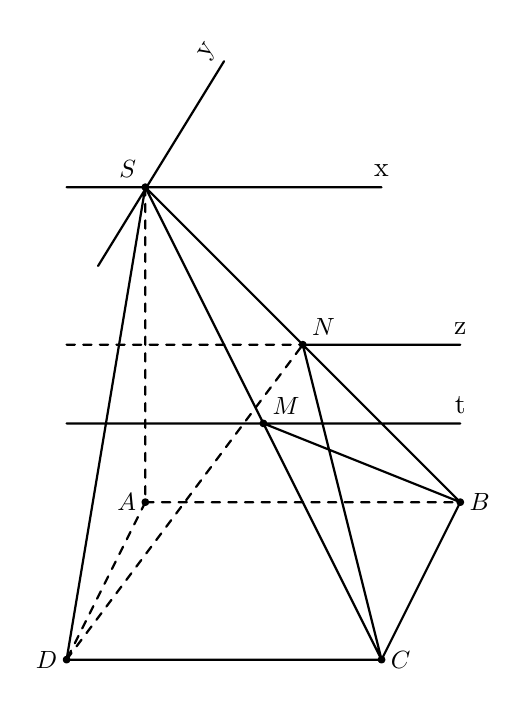
\begin{tikzpicture}[line join=round,line cap=round,>=stealth,thick]
     \coordinate (A) at  (-2,0);
     \coordinate (B) at  (2,0);
     \coordinate (C) at  (1,-2);
     \coordinate (D) at (-3,-2); 
     \coordinate (S) at  (-2,4);
      \coordinate (M) at (-0.5,1);
     \coordinate (N) at  (0,2);
      \coordinate (E) at (-3,4);
      \coordinate (F) at (1,4);
     \coordinate (G)  at (-2.6,3);
     \coordinate (H) at (-1,5.6); 
     \coordinate  (I) at (-3,1);
      \coordinate (J) at (2,1);
     \coordinate  (K) at (-3,2);
     \coordinate (L) at (2,2); 
      \draw[dashed](S)--(A)
      (A)--(D) 
      (A)--(B) 
       (D)--(N)
      (K)--(N); 
     \draw  (S)--(D)
       (S)--(C)
       (S)--(B)
      (D)--(C) 
       (C)--(B)
      (I)--(J) 
      (N)--(L) 
       (E)--(F)
      (G)--(H) 
      (M)--(B) 
       (C)--(N);
     \foreach \i  in {S,A,B,C,D,N,M}{\draw[fill=](\i) circle (1pt);}
     \foreach  \i in {N,M}{\draw (\i) node[scale=0.9,above right]{$\i$};}
     \foreach \i in {S}{\draw  (\i) node[scale=0.9,above left]{$\i$};}
     \foreach \i  in {A,D}{\draw (\i) node[scale=0.9,left]{$\i$};}
     \foreach  \i in {B,C}{\draw (\i) node[scale=0.9,right]{$\i$};}
     \path  (S)--(H) node [above,sloped,pos=1] {y};
     \path (E)--(F) node [above,sloped,pos=1]  {x};
     \path (K)--(L) node [above,sloped,pos=1] {z}; 
     \path (I)--(J) node [above,sloped,pos=1]  {t};
    \end{tikzpicture}
  \end{center}
  \begin{itemchoice}
   \itemch \textbf{Đúng}. 
   $ 
   \text{Ta có} \heva{&AB \parallel CD \\& AB \subset(SAB) \\ &CD \subset(SCD) \\ &S \in(SAB) \cap(SCD)} \quad  \Rightarrow\heva{&Sx=(SAB) \cap(SCD) \\ &Sx\parallel AB \parallel CD.}
    $
   \itemch \textbf{sai}. 
   $\text{Ta có} \heva{&AD \parallel BC \\  &AD \subset(SAD) \\ &BC \subset(SBC) \\ &S \in(SAD) \cap(SBC)} \Rightarrow\heva{&Sy=(SAD) \cap(SCD) \\ &Sy \parallel AD \parallel BC.}$.
    \itemch \textbf{Đúng}
   $\text{Ta  có} \heva{&AB \parallel CD \\& AB \subset(MAB) \\ &CD \subset(SCD) \\ &M \in(MAB) \cap(SCD)} \Rightarrow\heva{&Mt=(MAB) \cap(SCD) \\ &Mt \parallel AB \parallel CD.}$
   \itemch \textbf{Đúng}. $\text{Ta có} \heva{&AB \parallel CD \\  &AB \subset(SAB) \\ &CD \subset(NCD) \\ &N \in(SAB) \cap(NCD)} \Rightarrow\heva{&Nz=(SAB) \cap(NCD) \\ &Nz \parallel AB \parallel CD.}$
  \end{itemchoice}
 } 
\end{ex}

% nguồn: Ok_dungsai_lop11_Lan1
\begin{ex}%[1H4H2-2]%[ma:c9168be7]
 Cho hình chóp $S.ABCD$ có đáy  là hình bình hành. Khi đó:
  \choiceTF
  {\True  $AB$ song song $CD$}
  {\True $SA$ cắt  $SC$}
   {$SA$ song song $BC$}
  {\True  $SC$ chéo nhau $AB$}
 \loigiai{ 
  \begin{center}
   \begin{tikzpicture}[line join=round,line cap=round,>=stealth,scale=0.5,font=\footnotesize]
     \foreach \x/\y/\n in {0/0/A,-2.5/-2/B,6/0/D} \coordinate (\n) at  (\x,\y);
      \coordinate (C) at ($(B)+(D)-(A)$);
     \coordinate (S)  at ($(A)+(1,4)$);
     \draw (S)--(B)--(C)--(D)--(S)--(C); 
     \draw[dashed]  (S)--(A)--(D)
       (A)--(B);
      \foreach \t/\g in {A/150,B/-150,C/-30,D/30,S/90}{
      \draw[fill=black]  (\t) circle (1pt) node[shift={(\g:7pt)}]{$ \t $};
     } 
    \end{tikzpicture}
  \end{center}
  \begin{itemchoice}
   \itemch Đúng. Ta có $AB$ và $CD$ cùng nằm trong một mặt  phẳng và không có điểm chung nên $AB$ song song với $CD$ (hai cạnh đối của hình bình hành thì song song với nhau).
   \itemch Đúng. Hai đường thẳng $SA$ và  $SC$ cắt nhau tại $S$.
   \itemch Sai. Hai đường thẳng $SA$  và $BC$ không đồng phẳng, vì vậy $SA$ và $BC$ là hai đường thẳng chéo nhau.
   \itemch Đúng. $SC$ chéo nhau  $AB$.
  \end{itemchoice}
 } 
\end{ex}

% nguồn: Ok_dungsai_lop11_Lan1
\begin{ex}%[1H4H2-2]%[ma:46e00e49]
 Cho hình chóp $S.ABCD$ có đáy là hình bình hành tâm $O$.  Gọi $N$ là trung điểm của cạnh $SC$. Lấy điểm $M$ đối xứng với $B$ qua $A$. $ OM $ cắt $ AD$ tại $ K $, gọi giao điểm $G$ của đường thẳng $MN$ với mặt phẳng $\left(SAD\right)$.
  \choiceTF
  {\True $MD \parallel  AC$}
  {Đường thẳng $ ON  $ và $ SA $ cắt nhau}
  {\True $GK \parallel  ON$}
  {Tỉ số  $\dfrac{GM}{GN}=3$}
  \loigiai{
  \begin{center}
   \begin{tikzpicture}[>=stealth,line join=round,line cap = round,scale=1,font=\footnotesize]
      \def\ad{2}
      \def\ab{4}
      \def\h{4}
      \def\gocA{-80}
      \path
      (0,0) coordinate  (A)
      (\gocA:\ad) coordinate (D) 
      (\ab,0)  coordinate (B)
      ($(B)+(D)-(A)$) coordinate  (C)
      (2,\h) coordinate  (S)
      ($(S)!1/2!(C)$)  coordinate (N)
       ($(A)!1/2!(B)$) coordinate (I)
      (-\ab,0) coordinate (M) 
      (intersection of A--C and B--D)  coordinate (O)
      (intersection of M--O and A--D) coordinate  (K)
      (intersection of S--K and M--N) coordinate  (G);
      \foreach \p/\q in {S/90,A/180,B/0,C/-90,D/-90,N/0,M/180,O/-90,K/-120,G/90,I/90}
     \fill[black] (\p)  circle (1.0pt) node[shift={(\q:3.5mm)}]{$\p$};
     \draw  (S)--(B)--(C)--(S)--(D)--(M)--(G)
       (S)--(A)
       (D)--(C);
      \draw[dashed] (C)--(A)--(M)--(O)
      (A)--(B)--(D)--cycle  (N)--(G)--(K)
       (N)--(O)--(I);
    \end{tikzpicture}
  \end{center}
  \begin{itemchoice}
   \itemch \textbf{Đúng}. Xét tứ giác $AMDC$  có $\heva{&AM\parallel DC \\&AM=DC.}$\\
   Suy ra tứ giác  $AMDC$ là hình bình hành, nên $MD \parallel AC$.
   \itemch \textbf{Sai}. Vì $O$ là trung điểm $AC$, $N$ là trung điểm $SC$ nên  $ON \parallel SA$ (tính chất đường trung bình).
   \itemch \textbf{Đúng}. Ta có $\heva{&ON \parallel SA\\& 
    ON\subset\left(OMN\right)\\&
   SA\subset\left(SAD\right)\\& 
   \left(OMN\right)\cap\left(SAD\right)= GK}\Rightarrow GK\parallel ON \parallel  SA$.
   \itemch \textbf{Sai}. Áp dụng định lí Thalès cho $ \triangle MON $  với $GK\parallel ON$, ta có
   $\dfrac{GM}{GN}=\dfrac{KM}{KO}\quad(1)$.  \\
   Gọi $I$ là trung điểm của $AB$, vì  $O$ là trung điểm của $BD$ nên theo tính chất đường trung bình ta suy ra $OI\parallel AD$.
    \\ Mặt khác theo định lí Thalès ta lại có
   $\dfrac{KM}{KO}=\dfrac{AM}{AI}=\dfrac{AB}{AI}=2 \quad(2)$.\\ 
   Từ $ (1) $ và $ (2) $, ta có $\dfrac{GM}{GN}=2$. 
  \end{itemchoice}
 } 
\end{ex}

% nguồn: Ok_dungsai_lop11_Lan1
\begin{ex}%[1H4H2-2]%[ma:6ed74609]
 Cho hình chóp $S.ABCD$, có đáy $ABCD$ là một hình bình hành tâm $O$. Gọi $I$, $K$ lần lượt là trung điểm của $SB$ và  $SD$. Khi đó
  \choiceTF
  {\True $SO$ là giao  tuyến của $(SAC)$ và $(SBD)$}
  {Giao điểm $J$ của $SA$ với $(CKB)$ thuộc đường thẳng đi qua $K$ và  song song với $DC$}
  {\True Giao tuyến của $(OIA)$ và $(SCD)$ là đường thẳng đi qua $C$ và song  song với $SD$}
  {\True $CD \parallel  IJ$}
 \loigiai{ 
  \begin{center}
   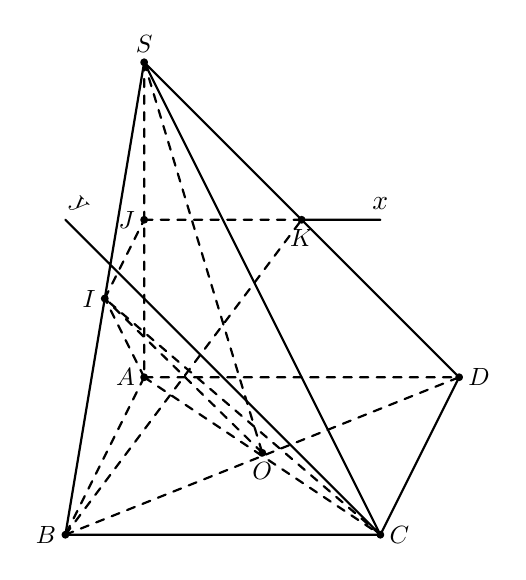
\begin{tikzpicture}[line join=round,line cap=round,>=stealth,thick]
     \coordinate  (A) at (-2,0);
      \coordinate (B) at (-3,-2);
     \coordinate  (C) at (1,-2);
     \coordinate (D) at (2,0); 
     \coordinate (S) at  (-2,4);
     \coordinate  (J) at (-2,2);
     \coordinate  (F) at (1,2);
     \coordinate  (I) at (-2.5,1);
     \coordinate (O) at (-0.5,-0.96); 
     \coordinate (K)  at (0,2);
     \coordinate (H) at  (-3,2);
     \draw[dashed](S)--(A) 
      (A)--(B) 
       (A)--(D)
       (B)--(D)
       (A)--(C)
      (S)--(O) 
       (I)--(J)
      (J)--(K) 
       (B)--(K)
       (O)--(I)
      (C)--(I) 
      (A)--(I); 
     \draw  (S)--(B)
      (S)--(C) 
       (S)--(D)
       (B)--(C)
      (C)--(D) 
      (C)--(H) 
      (K)--(F); 
     \foreach \i  in {S,A,B,C,D,O,I,K,J}{\draw[fill=](\i) circle (1pt);}
     \foreach \i  in {S}{\draw (\i) node[scale=0.9,above]{$\i$};}
     \foreach \i in {J,I,A,B}{\draw  (\i) node[scale=0.9,left]{$\i$};}
      \foreach \i in {D,C}{\draw (\i) node[scale=0.9,right]{$\i$};}
     \foreach \i in {O,K}{\draw (\i) node[scale=0.9,below]{$\i$};} 
     \path (K)--(F) node [above,sloped,pos=1] {$x$}; 
      \path (C)--(H) node [above,sloped,pos=1] {y};
    \end{tikzpicture}
  \end{center}
  \begin{itemchoice}
   \itemch \textbf{Đúng}. Ta có $\heva{&O \in AC  \subset(SAC) \\ &O \in BD \subset(SBD)} \Rightarrow O \in(SAB) \cap(SCD).$\\
   Mà $S \in(SAB) \cap(SCD)$ 
   $\Rightarrow SO=(SAC) \cap(SBD)$. 
    \itemch \textbf{sai}. Tứ giác $ABCD$ là hình bình hành nên $AB \parallel CD$, $AD \parallel BC$.\\
   Ta có $\heva{&AD \parallel CB \\ &AD \subset(SAD) \\ &BC \subset(SBC) \\ &K \in(KBC) \cap(SAD)} \Rightarrow\heva{&Kx=(KBC) \cap(SAD) \\ &Kx \parallel AD \parallel  BC}.$\\
   Trong $(SAD)$ gọi $J=Kx \cap SA$, có $\Rightarrow\heva{&J \in SA \\&J \in Kx \subset(BKC)} \Rightarrow  J=SA \cap(BKC)$.
   \itemch \textbf{Đúng}. Có $OI$ là đường trung  bình của $\triangle SBD \Rightarrow OI \parallel SD$.\\
   Ta có $\heva{&OI \parallel SD \\ &OI \subset(OIA) \\& SD \subset(SCD) \\& C \in(OIA) \cap(SCD)} \Rightarrow\heva{&Cy=(OIA) \cap(SCD) \\& Cy  \parallel SD \parallel OI.}$
   \itemch \textbf{Đúng}. Ta  có
   $IJ  \parallel AB$ ($IJ$ là đường trung bình của $\triangle SAB$).\\
    $AB \parallel CD$ (tứ giác $ABCD$ là hình bình hành).\\ $\Rightarrow CD \parallel IJ$.
  \end{itemchoice}
  }
\end{ex}

% nguồn: Ok_dungsai_lop11_Lan1
\begin{ex}%[1H4H2-2]%[ma:e5a6e0a6]
 \immini{Cho tứ diện $ABCD$ có $M$, $N$ lần lượt là trung điểm của $AB$,  $AC$. Khẳng định nào đúng?
 \choiceTF 
  {\True $MN$  song song $BC$}
  {$AN$ song song $CD$} 
  {\True $MN$ song song $(ABC)$} 
  {$DC$ song  song $(AMN)$}}{
  \begin{tikzpicture}[scale=1.21,font=\footnotesize,line join=round,line cap=round,>=stealth]
     \coordinate[label=left:$B$] (B) at (0,0);
    \coordinate[label=right:$D$]  (D) at (4,0);
     \coordinate[label=below:$C$] (C) at (2,-1.4);
     \coordinate[label=above:$A$] (A) at (2,3);
    \coordinate[label=above  left:$M$] (M) at ($(A)!0.5!(B)$);
    \coordinate[label=right:$N$] (N) at ($(A)!0.5!(C)$); 
    \draw (B)--(C)--(D)--(A)--cycle  (A)--(C)
     (M)--(N); 
    \draw[dashed] (B)--(D); 
    \foreach  \diem in {B,C,D,A,M,N}\fill (\diem) circle (1pt);
   \end{tikzpicture}
   }
  \loigiai{
  \begin{itemchoice}
   \itemch Đúng.\\ Vì $MN$ là đường trung  bình của tam giác $ABC$.
    \itemch Sai.\\ Vì $AN$ và $CD$ có $C$ là điểm chung.
   \itemch Đúng.\\ Vì $\heva{&IK \parallel MP\\& IJ \parallel MN} \Rightarrow  (IJK) \parallel (ABC)$.
   \itemch Sai.\\ Vì $DC$  và $(AMN)$ có $C$ là điểm chung.
 \end{itemchoice}}
\end{ex}

% nguồn: Ok_dungsai_lop11_Lan2
\begin{ex}%[1H4H2-2]%[ma:4b1434b2]
	Cho tứ diện $ABCD$. Gọi $I$ và $J$ lần lượt là trọng tâm của các tam  giác $ABD$ và $ABC$. Xét tính đúng sai của các mệnh đề sau
	 \choiceTF
		{\True $IJ$ song song với $CD$} 
		{$IJ$ song song với $AB$} 
		 {\True $IJ$ song song $MN$}
		{$IJ$  cắt $AB$}
	\loigiai{ 
	\immini{ 
		Gọi $M$, $N$ lần lượt là trung điểm của $BD$,  $BC$\\
		$\Rightarrow MN$ là đường trung bình của  tam giác $BCD \Rightarrow MN\parallel CD$.\hfill $(1)$ \\
		Ta có $I$, $J$ lần  lượt là trọng tâm của các tam giác $ABD$ và $ABC$ nên $\dfrac{AI}{AM}=\dfrac{AJ}{AN}=\dfrac{2}{3}\Rightarrow IJ\parallel MN$.\hfill $(2)$ \\
		Từ $(1)$ và $(2)$ suy  ra $IJ\parallel CD$.
		 }
		{ 
		\begin{tikzpicture}[scale=1,font=\footnotesize,line join=round,line cap=round,>=stealth]
				\path  (0,0) coordinate (B)++(0:3) coordinate (C)++(-160:2) coordinate (D)
					(70:2.5) coordinate  (A)
					 ($(B)!.5!(D)$) coordinate (M)
					 ($(B)!.5!(C)$) coordinate (N)
					($(A)!2/3!(M)$) coordinate  (I)
					($(A)!2/3!(N)$) coordinate (J); 
				\draw (A)--(B)--(D)--(C)--cycle  (M)--(A)--(D);
				 \draw[dashed] (B)--(C)
					(A)--(N)--(M) 
					 (I)--(J);
				\foreach \diem/\vitri in  {A/120,B/180,C/0,D/-70,M/-100,N/40,I/150,J/20}{
					\fill (\diem)  circle (1pt)
					($(\diem)+(\vitri:2mm)$) node[scale=.8]{$\diem$}; 
				 }
			\end{tikzpicture}
		} 
		\begin{itemchoice}
			\itemch Đúng. Từ $(1)$  và $(2)$ suy ra $IJ\parallel CD$.
			\itemch Sai. $A$, $B$, $I$, $J$ không đồng phẳng nên $AB$ và $IJ$ không  song song.
			\itemch Đúng.  Theo $(2)$, ta có $IJ\parallel MN$.
			\itemch Sai. $A$, $B$, $I$, $J$ không đồng phẳng nên $AB$ và  $IJ$ không cắt nhau.
		\end{itemchoice}
	 }
\end{ex}

% nguồn: Ok_dungsai_lop11_Lan2
\begin{ex}%[1H4H2-2]%[ma:9cd0e5cf]
	Cho hình chóp $S.ABCD$ có đáy là hình  bình hành. Khi đó
	 \choiceTF
		{\True  $AB$ song song $CD$}
		{\True  $SA$ cắt $SC$}
		{$SA$ song  song $BC$}
		{\True $SC$ chéo nhau  $AB$}
	 \loigiai{
	\immini{\begin{itemchoice}
		\itemch Ta có $AB$ và $CD$ cùng nằm trong một mặt phẳng và không có điểm chung nên $AB$ song song với $CD$ (hai  cạnh đối của hình bình hành thì song song với nhau).
		\itemch Hai đường thẳng $SA$ và $SC$ cắt  nhau tại $S$.
		\itemch Hai  đường thẳng $SA$ và $BC$ không đồng phẳng, vì vậy $SA$ và $BC$ là hai đường thẳng chéo nhau.
		\itemch $SC$  chéo nhau $AB$.
	\end{itemchoice}}
	{\begin{tikzpicture}[scale=1,font=\footnotesize,line join=round,line cap=round,>=stealth]
		 \path
			(0,0)  coordinate (A)
			++(-140:2)  coordinate (B)
			 ++(0:3.5) coordinate (C)
			($(A)+(C)-(B)$)  coordinate (D)
			($(A)+(0,3)$) coordinate  (S);
		\foreach  \i in{B,C,D}{\draw (S)--(\i);};
		 \draw (B)--(C)--(D);
		\draw[dashed] (S)--(A)--(B) 
			 (A)--(D);
		 \foreach \i/\g in {A/-90,B/-90,C/-90,D/-90,S/90}
		\fill (\i) circle (1pt)+(\g:3mm)  node[scale=1]{$\i$};
	\end{tikzpicture}
	} 
} 
\end{ex}

% nguồn: Ok_dungsai_lop11_Lan2
\begin{ex}%[1H4H2-2]%[ma:69590a74]
	Cho hình chóp $S.ABCD$ có đáy  $ABCD$ là hình bình hành. Gọi $M$, $G$ lần lượt là các điểm thuộc cạnh $SB$, $SC$ sao cho $\dfrac{SM}{SB}=\dfrac{SG}{SC}=\dfrac{2}{3}$. Xét tính đúng sai của các mệnh đề sau
	\choiceTF 
		{\True $MG\parallel AD$} 
		{\True $MG\parallel BC$} 
		{$MG\parallel  AB$}
		{$MG\parallel AC$} 
	 \loigiai{
	\immini{ 
		\begin{itemchoice}
			\itemch Đúng. Vì $\dfrac{SM}{SB}=\dfrac{SG}{SC}=\dfrac{2}{3}$ nên theo định lí Ta-let, ta  có \break $MG\parallel BC$, mà $BC\parallel AD$ suy ra $MG\parallel AD$.
			\itemch Đúng. 
			\itemch Sai. $A$, $B$, $M$, $G$ không đồng  phẳng.
			\itemch Sai. $A$, $C$, $M$, $G$ không  đồng phẳng.
		\end{itemchoice}
		} 
		 {
		\begin{tikzpicture}[scale=1,font=\footnotesize,line join=round,line cap=round,>=stealth]
				\path (0,0) coordinate (A)++(0:3) coordinate  (B)++(-140:1.5) coordinate (C)
					 ($(A)-(B)+(C)$) coordinate (D)
					 (80:3) coordinate (S)
					($(S)!2/3!(B)$) coordinate (M) 
					($(S)!2/3!(C)$) coordinate  (G);
				\draw[dashed] (S)--(A)--(B) 
					 (A)--(D);
				\draw  (B)--(C)--(D)--(S)--cycle (S)--(C)
					 (M)--(G);
				\foreach \diem/\vitri in {A/160,B/20,C/-20,D/200,S/30,M/20,G/190}{ 
					\fill (\diem)  circle (1pt)
					($(\diem)+(\vitri:2mm)$)  node[scale=.8]{$\diem$};
				} 
			\end{tikzpicture}
		} 
	} 
\end{ex}

% nguồn: Ok_dungsai_lop11_Lan2
\begin{ex}%[1H4H2-2]%[ma:972793c6]
	Cho hình chóp $S.ABCD$ có đáy $ABCD$ là hình bình hành, $AC$ cắt $BD$ tại $O$. Gọi $M$ là trung điểm của $SC$. Xét tính đúng sai của  các mệnh đề sau
	\choiceTF 
		{$OM\parallel SD$} 
		{\True $AB\parallel  CD$}
		 {$OM\parallel SB$}
		{\True $OM\parallel SA$} 
	 \loigiai{
	\immini{ 
		\begin{itemchoice}
			\itemch Sai. $S$, $D$, $M$, $O$ không đồng  phẳng.
			\itemch Đúng. $ABCD$ là hình bình  hành.
			 \itemch Sai. $S$, $B$, $M$, $O$ không đồng phẳng.
			\itemch Đúng.  \\
			$M$, $O$ lần lượt là trung điểm  của $SC$, $AC$\\
			$\Rightarrow MO$  là đường trung bình của $\triangle SAC \Rightarrow MO\parallel SA$.
		\end{itemchoice}
		 }
		{ 
		\begin{tikzpicture}[scale=1,font=\footnotesize,line join=round,line cap=round,>=stealth]
				\path (0,0) coordinate (A)++(0:3) coordinate (B)++(-150:1.5) coordinate  (C)
					($(A)-(B)+(C)$) coordinate (D) 
					(80:3) coordinate (S)++(0:2)  coordinate (p)
					(intersection of A--C and B--D) coordinate (O) 
					($(S)!.5!(C)$) coordinate  (M);
				\draw[dashed]  (S)--(A)--(B)
					(C)--(A)--(D)--(B) 
					 (M)--(O);
				\draw  (B)--(C)--(D)--(S)--cycle (S)--(C);
				 \foreach \diem/\vitri in {A/160,B/20,C/-20,D/200,S/90,O/-90,M/10}{
					\fill (\diem)  circle (1pt)
					 ($(\diem)+(\vitri:2mm)$) node[scale=.8]{$\diem$};
				} 
			\end{tikzpicture}
		} 
	} 
\end{ex}

% nguồn: Ok_dungsai_lop11_Lan2
\begin{ex}%[1H4H2-2]%[ma:50ddc413]
	Cho hình chóp $S.ABCD$ có đáy $ABCD$ là hình bình hành, tâm $O$. Gọi $I$, $J$ lần lượt là trọng tâm của  các tam giác $SAB$ và $SAD$. Gọi $M$, $N$ lần lượt là trung điểm của $AB$, $AD$. Xét tính đúng sai của các mệnh đề sau
	\choiceTF 
		{\True $IJ$ song song với đường thẳng  $MN$}
		{\True $IJ$ song song với đường  thẳng $BD$}
		{$IJ$ song  song với đường thẳng $BC$}
		{$IJ$  song song với đường thẳng $SO$}
	\loigiai{ 
	 \immini{
		\begin{itemchoice}
			\itemch Đúng. Ta  có $\dfrac{SI}{SM}=\dfrac{SJ}{SN}=\dfrac{2}{3} \Rightarrow IJ\parallel MN$.
			\itemch Đúng. Ta có $\heva{&MN\parallel  IJ \\ &MN\parallel BD} \Rightarrow IJ\parallel BD$.
			\itemch Sai. $I$,  $J$, $B$, $C$ không đồng phẳng.
			\itemch Sai. $I$, $J$, $S$,  $O$ không đồng phẳng.
		\end{itemchoice}
		} 
		{ 
		\begin{tikzpicture}[scale=1,font=\footnotesize,line join=round,line cap=round,>=stealth]
				\path (0,0)  coordinate (A)++(0:3.5) coordinate (B)++(-150:2.2) coordinate (C)
					($(A)-(B)+(C)$)  coordinate (D)
					 (80:3) coordinate (S)++(0:2) coordinate (p)
					(intersection of  A--C and B--D) coordinate (O)
					($(A)!.5!(B)$) coordinate  (M)
					 ($(A)!.5!(D)$) coordinate (N)
					($(S)!2/3!(M)$)  coordinate (I)
					 ($(S)!2/3!(N)$) coordinate (J);
				\draw[dashed] (O)--(S)--(A)--(B) 
					 (C)--(A)--(D)--(B)
					(M)--(S)--(N)--cycle (I)--(J); 
				\draw (B)--(C)--(D)--(S)--cycle  (S)--(C);
				\foreach \diem/\vitri in {A/150,B/20,C/-20,D/200,S/90,O/-80,M/45,N/150,I/0,J/-70}{ 
					\fill (\diem) circle  (1pt)
					($(\diem)+(\vitri:2mm)$)  node[scale=.8]{$\diem$};
				} 
			\end{tikzpicture}
		 }
	 }
\end{ex}

% nguồn: Ok_dungsai_lop11_Lan2
\begin{ex}%[1H4H2-2]%[1H4H1-3]%[ma:f5dbac8d]
	Cho tứ diện $ABCD$ gọi $I$ và $J$ lần lượt là trung điểm  của $AD$ và $AC$, $G$là trọng tâm của tam giác $BCD$
	\choiceTF 
		{\True $IJ\parallel CD$} 
		{Giao tuyến của hai mặt phẳng $(GIJ)$ và $(BCD)$  là đường thẳng qua $G$ và song song với $BC$}
		{Cho biết $CD=6$. Biết $(GIJ)$ cắt $BC, BD$ lần lượt tại $M$ và $N$. Khi  đó $2IJ+3MN=17$}
		{Cho biết $CD=6$. Biết $(GIJ)$ cắt $BC, BD$ lần lượt  tại ${M}$ và ${N}$. Khi đó $3IJ+2MN=18$}
	 \loigiai{
		\begin{center}
			\begin{tikzpicture}[thick,font=\scriptsize]
					\def\a{4} 
					\path (0:0)  coordinate (B)
						 (0:5) coordinate (D)
						(-30:3.5) coordinate (C) 
						(45:4) coordinate  (A)
						(barycentric cs:A=1,D=1)  coordinate (I)
						(barycentric cs:A=1,C=1) coordinate (J) 
						(barycentric cs:D=1,C=1) coordinate (E) 
						(barycentric cs:B=1,C=1,D=1)  coordinate (G)
						(barycentric cs:B=1,C=2) coordinate  (M)
						(barycentric cs:B=1,D=2) coordinate (N); 
					\draw[dashed,thin] (E)--(B)--(D) 
						 (M)--(N);
					\draw[]  (B)--(A)--(D)
						 (A)--(C)
						 (B)--(C)--(D)
						(I)--(J); 
					\foreach \x/\y in  {A/90,B/180,C/-90,D/0,I/0,J/180,G/90,E/-90,M/-90,N/90}
					 \fill[black] (\x) circle (1pt)
						($(\y:3mm)+(\x)$)  node {$\x$};
				\end{tikzpicture}
		\end{center}
		\begin{itemchoice}
			\itemch Đúng.\\ 
			Dễ thầy $IJ$  là đường trung bình của $\triangle ACD$ nên $IJ\parallel CD$.
			\itemch  Sai.\\
			Xác định giao tuyến của hai mặt  phẳng $(GIJ)$ và $(BCD)$:\\
			Vì $IJ$ là đường  trung bình của tam giác $ACD$ nên $IJ\parallel CD$.\\
			 Ta có $\heva{
			 &G\in (GIJ)\cap (BCD) \\
			&IJ\parallel CD \\ 
			&IJ\subset (GIJ),\, CD\subset (BCD) } $ $\Rightarrow Gx=(GIJ)\cap(BCD)$,  trong đó $Gx$ là đường thẳng qua $G$ và $Gx\parallel IJ\parallel CD$.
			\itemch  Sai.\\
			Trong mặt phẳng $(BCD)$, kẻ $Gx$ song song $CD$ cắt $BC$ tại $M$,  cắt $BD$ tại $N$.\\
			-Tính  $2IJ+3MN$\\
			Gọi $E$ là trung điểm $CD$, theo định lí Thalès, ta  có:\\
			$\dfrac{BM}{BC} =\dfrac{BG}{BE} =\dfrac{2}{3}$ vì  $(GM\parallel CE)$; $\dfrac{MN}{CD}=\dfrac{BM}{BC}$ vì $(MN\parallel CD)$\\
			Suy ra $\dfrac{MN}{CD}=\dfrac{2}{3}$ hay $MN=\dfrac{2}{3} CD =\dfrac{2}{3} \cdot  6=4$.\\
			 Vì $IJ$ là đường trung bình tam giác $ACD$ nên $IJ=\dfrac{1}{2} CD =\dfrac{1}{2} \cdot 6=3$.\\
			 Do đó $2IJ+3MN=2 \cdot 3+3 \cdot 4=18$.
			\itemch Sai.\\ 
			$3IJ+2MN=3\cdot  3+2\cdot 4=17$
		\end{itemchoice}
	} 
\end{ex}

% nguồn: Ok_dungsai_lop11_Lan2
\begin{ex}%[1H4H2-2]%[ma:b3af978b]
	Cho hình chóp $S.ABCD$ có đáy  là hình bình hành.
	\choiceTF 
		{\True $AB$ song song $CD$} 
		 {\True $SA$ cắt $SC$}
		{$SA$ song song $BC$} 
		{\True $SC$  chéo nhau $AB$}
	\loigiai{ 
		\begin{center}
			\begin{tikzpicture}[scale=0.8,font=\footnotesize,line join=round,line cap=round,>=stealth]
					\def\a{3} 
					\coordinate (A) at  (0,0);
					\coordinate  (B) at (\a*1.3,0);
					\coordinate (D)  at ($(A)+(\a*0.4,\a*0.5)$);
					\coordinate (C) at ($(B)+(D)-(A)$); 
					\coordinate (S) at ($(\a*0.6,\a*1.5)$); 
					 \draw (S)--(B)--(C)--(S)--(A)--(B);
					\draw[dashed] (D)--(A) 
						 (S)--(D)--(C);
					\foreach \x/\label/\g in  {S/\(S\)/90,B/\(B\)/-90,C/\(C\)/-80,D/\(D\)/140,A/\(A\)/-90}
					\fill (\x) circle  (1pt)
						 ($(\x)+(\g:3mm)$) node{\small $\x$};
				\end{tikzpicture}
		\end{center}
		\begin{itemchoice}
			\itemch  \textbf{Sai} \\
			Ta có $AB$ và $CD$ là hai cạnh đối của  hình bình hành thì song song với nhau.
			\itemch \textbf{Đúng} \\ 
			Hai đường thẳng $SA$ và $SC$  cắt nhau tại $S$.
			\itemch  \textbf{Sai}\\
			Hai đường thẳng $SA$ và $BC$ không đồng phẳng, vì vậy $SA$ và  $BC$ là hai đường thẳng chéo nhau.
			\itemch \textbf{Sai}  \\
			 $SC$ chéo nhau $AB$.
		\end{itemchoice}
	} 
\end{ex}

% nguồn: Ok_dungsai_lop11_Lan2
\begin{ex}%[1H4H2-2]%[ma:f858f843]
	Cho hình chóp $S.ABCD$ có đáy $ABCD$ là hình vuông. Gọi $M$, $N$ lần lượt là trung điểm  của $SA$ và $SC$. Xét tính đúng sai của các mệnh đề sau
	 \choiceTF
		{$MN\parallel  AD$}
		{$MN\parallel  BC$}
		{$MN\parallel AB$} 
		{\True $MN\parallel  AC$}
	\loigiai{ 
	\immini{ 
		$M$, $N$ lần lượt là trung điểm  của $SA$, $SC$\\
		$\Rightarrow$ $MN$ là đường trung bình của $\triangle SAC \Rightarrow MN\parallel  AC$.
		\begin{itemchoice}
			\itemch Sai. $A$, $D$,  $M$, $N$ không đồng phẳng.
			\itemch Sai. $C$, $B$, $M$, $N$ không đồng phẳng. 
			\itemch Sai.  $A$, $B$, $M$, $N$ không đồng phẳng.
			\itemch Đúng. $MN$ là đường  trung bình $\triangle SAC$.
		\end{itemchoice}
		 }
		 {
		\begin{tikzpicture}[scale=1,font=\footnotesize,line join=round,line cap=round,>=stealth]
				 \path (0,0) coordinate (A)++(0:3) coordinate (B)++(-150:1.5) coordinate (C)
					($(A)-(B)+(C)$)  coordinate (D)
					(80:3) coordinate  (S)++(0:2) coordinate (p)
					(intersection of A--C and  B--D) coordinate (O)
					($(S)!.5!(A)$) coordinate (M) 
					($(S)!.5!(C)$) coordinate (N); 
				 \draw[dashed] (S)--(A)--(B)
					(C)--(A)--(D) 
					 (M)--(N);
				\draw  (B)--(C)--(D)--(S)--cycle (S)--(C);
				\foreach \diem/\vitri in {A/160,B/20,C/-20,D/200,S/90,O/-90,M/150,N/20}{ 
					\fill (\diem) circle (1pt) 
					($(\diem)+(\vitri:2mm)$)  node[scale=.8]{$\diem$};
				 }
			\end{tikzpicture}
		 }
	 }
\end{ex}

% nguồn: Ok_dungsai_lop11_Lan2
\begin{ex}%[1H4H2-2]%[ma:4ec84a87]
	Cho hình chóp $S.ABCD$ có đáy là hình bình hành $ABCD$ tâm $O$.  Gọi $G$, $K$ lần lượt là trọng tâm của $\triangle SAD$ và $\triangle ACD$. Xét tính đúng sai của các mệnh đề sau
	 \choiceTF
		{$KG$  song song với đường thẳng $SB$}
		{\True  $KG$ song song với đường thẳng $SC$}
		{$KG$ song  song với đường thẳng $SA$}
		 {$KG$ song song với đường thẳng $SO$}
	 \loigiai{
	\immini{ 
		Gọi $M$ là trung điểm  của $AD$.\\
		Ta có $\dfrac{MG}{MS}=\dfrac{MK}{MC}\left(=\dfrac{1}{3}\right)\Rightarrow GK\parallel SC$. 
		\begin{itemchoice}
			\itemch Sai. Vì $K$, $G$, $S$,  $B$ không đồng phẳng.
			\itemch Đúng. Vì $GK$ là đường trung  bình $\triangle MSC$.
			\itemch Sai. Vì $K$, $G$, $S$,  $A$ không đồng phẳng.
			\itemch Sai. Vì $K$,  $G$, $S$, $O$ không đồng phẳng.
		\end{itemchoice}
		} 
		 {
		\begin{tikzpicture}[scale=1,font=\footnotesize,line join=round,line cap=round,>=stealth]
				\path (0,0) coordinate (A)++(0:3) coordinate (B)++(-150:2.2) coordinate (C) 
					($(A)-(B)+(C)$) coordinate (D) 
					(80:3) coordinate (S)++(0:2)  coordinate (p)
					(intersection of A--C and B--D) coordinate  (O)
					($(A)!.5!(D)$)  coordinate (M)
					($(S)!2/3!(M)$) coordinate  (G)
					 ($(C)!2/3!(M)$) coordinate (K);
				 \draw[dashed] (S)--(A)--(B)
					 (C)--(A)--(D)--(B)
					 (M)--(S)
					(C)--(M) 
					 (G)--(K);
				\draw  (B)--(C)--(D)--(S)--cycle (S)--(C);
				 \foreach \diem/\vitri in {A/150,B/20,C/-20,D/200,S/90,O/90,M/170,G/0,K/-90}{
					\fill (\diem)  circle (1pt)
					($(\diem)+(\vitri:2mm)$)  node[scale=.8]{$\diem$};
				 }
			\end{tikzpicture}
		 }
	} 
\end{ex}

% nguồn: Ok_dungsai_lop11_Lan2
\begin{ex}%[1H4H2-2]%[ma:c0b5bf62]
	Cho hình chóp $S.ABCD$ có đáy là hình chữ nhật. Gọi $M$, $N$, $E$, $F$ lần lượt là trọng tâm các tam giác $SAB$, $SBC$, $SCD$ và $SDA$. Gọi $M'$, $N'$, $E'$, $F'$  lần lượt là trung điểm của $AB$, $BC$, $CD$, $DA$. Khi đó
	\choiceTF 
		{\True Hai  đường thẳng $MN$ và $M'N'$ song song với nhau}
		{Hai đường thẳng $MN$  và $EF$ chéo nhau với nhau}
		{\True Hai đường thẳng  $MF$ và $NE$ chéo nhau với nhau}
		{Tứ giác $MNEF$ là hình chữ nhật} 
	 \loigiai{
		\begin{center}
			\begin{tikzpicture}[scale=1.3,font=\footnotesize,line join=round,line cap=round,>=stealth]
					 \path
						(0,0)  coordinate (A)
						++(-140:2) coordinate (B) 
						++(0:4.5) coordinate (C) 
						 ($(A)+(C)-(B)$) coordinate (D)
						($(A)!1/2!(C)$)  coordinate (O)
						($(O)+(0,3.5)$) coordinate (S); 
					\coordinate  (M') at ($(A)!0.5!(B)$);
					\coordinate (N') at ($(C)!0.5!(B)$); 
					 \coordinate (E') at ($(C)!0.5!(D)$);
					\coordinate (F')  at ($(A)!0.5!(D)$);
					\coordinate (M)  at ($(S)!0.5!(M')$);
					\coordinate (N) at ($(S)!0.5!(N')$); 
					\coordinate  (E) at ($(S)!0.5!(E')$);
					\coordinate  (F) at ($(S)!0.5!(F')$);
					\coordinate (I) at ($(M)!0.5!(E)$); 
					\foreach \i in{B,C,D}{\draw (S)--(\i);}; 
					\foreach \j in{N',E'}{\draw (S)--(\j);}; 
					 \draw (B)--(C)--(D);
					\draw[dashed] (S)--(A)--(B) 
						 (C)--(A)--(D)--(B)
						(S)--(O) 
						(E')--(S)--(M') 
						(M)--(N)--(E)--(F)--(M) 
						 (M')--(N')--(E')--(F')--(M')
						(M)--(E) 
						 (N)--(F)
						 (S)--(F');
					\foreach \i/\g in  {A/-90,B/-90,C/-90,D/-90,O/-90,S/90,I/0,M/180,N/-70,E/0,F/0,M'/-80,N'/-90,E'/0,F'/-90}
					\fill (\i)  circle (1pt)+(\g:3mm) node[scale=1]{$\i$};
				\end{tikzpicture}
		\end{center}
		\begin{itemchoice}
			\itemch Ta có $\dfrac{SM}{SM'}=\dfrac{2}{3};\ \dfrac{SN}{SN'}=\dfrac{2}{3} \Rightarrow \dfrac{SM}{SM'}=\dfrac{SN}{SN'} \Rightarrow MN\parallel M'N' \qquad  (1)$.
			\itemch Tương tự $\dfrac{SE}{SE'}=\dfrac{SF}{SF'}=\dfrac{2}{3} \Rightarrow EF\parallel E'F'\qquad (2)$ và $\heva{&M'N' \parallel AC\\&E'F' \parallel AC} \Rightarrow  M'N' \parallel E'F'\qquad (3)$.\\
			Từ $(1)$, $(2)$ và $(3)$ suy  ra $MN\parallel EF$.
			\itemch Chứng minh hoàn toàn tương  tự như trên, ta có $MN\parallel M'F';\ M'F' \parallel N'E';\ N'E' \parallel NE$ nên $MF\parallel NE$.
			\itemch  Tứ giác $MNEF$ có $\heva{&MN\parallel EF\\&MF\parallel NE}$ nên $MNEF$ là hình bình hành.
		\end{itemchoice}
	} 
\end{ex}

% nguồn: Ok_dungsai_lop11_Lan1
\begin{ex}%[1H4V2-2]%[1H4V3-2]%[ma:348dec16]
 Cho  hình chóp $S.ABCD$ có đáy $ABCD$ là hình bình hành tâm $O$. Gọi $M$, $N$ lần lượt là trung điểm của $SA$ và $SD$. Khi đó:
 \choiceTF 
   {\True $MN \parallel BC$}
  {$OM \parallel SB$} 
  {\True  $MN \parallel (ABCD)$}
   {\True $NO \parallel (SBC)$}
 \loigiai{ 
  \begin{center}
   \begin{tikzpicture}[>=stealth,scale=0.7,line join = round,line cap = round]
      \coordinate (A) at (2,0);
     \coordinate (B) at  (8,0);
     \coordinate (C) at (6,-3); 
     \coordinate (D) at  (0,-3);
     \coordinate (S)  at (3,6);
     \coordinate (O)  at (4,-1.5);
     \coordinate  (M) at (2.5,3);
     \coordinate  (N) at (1.5,1.5);
     \draw[fill=black]  (A) circle (1pt) node [left] {$A$};
     \draw[fill=black] (B) circle (1pt)  node [right] {$B$};
     \draw[fill=black] (C)  circle (1pt) node [right] {$C$};
     \draw[fill=black]  (D) circle (1pt) node [left] {$D$};
     \draw[fill=black] (S) circle (1pt) node  [above] {$S$};
      \draw[fill=black] (O) circle (1pt) node [below] {$O$};
     \draw[fill=black] (M) circle  (1pt) node [right] {$M$};
      \draw[fill=black] (N) circle (1pt) node [left] {$N$};
     \draw[dashed] (A)--(B); 
     \draw[dashed]  (A)--(D);
     \draw (C)--(B); 
     \draw[dashed] (A)--(C); 
     \draw[dashed]  (D)--(B);
     \draw  (C)--(D);
     \draw[dashed] (A)--(S); 
      \draw (S)--(B);
      \draw (S)--(C);
     \draw  (S)--(D);
      \draw[dashed] (M)--(N);
     \draw[dashed] (N)--(O); 
     \draw[dashed] (M)--(O); 
    \end{tikzpicture}
  \end{center}
  \begin{itemchoice}
   \itemch Ta có $MN$ là đường trung bình của tam giác $SAD$, suy ra $MN \parallel AD$. \\ 
    Mà $AD \parallel BC$, do đó $MN \parallel BC$.
   \itemch Dễ thấy $OM$ và $SB$ không đồng  phẳng do đó $OM$ không song song với $SB$.
   \itemch Ta có  $MN$ là đường trung bình của tam giác $SAD$, suy ra $MN \parallel AD$. \\
   Mà $AD  \subset (ABCD)$, do đó $MN \parallel (ABCD)$.
   \itemch  Ta có $NO$ là đường trung bình của tam giác $SBD$, suy ra $NO \parallel SB$. \\
   Mà $SB \subset  (SBC)$, do đó $NO \parallel (SBC)$.
  \end{itemchoice}
  }
\end{ex}

% nguồn: Ok_dungsai_lop11_Lan2
\begin{ex}%[1H4V2-2]%[ma:c7e8d3fb]
	Cho tứ diện  $ABCD$ có $I$, $J$ theo thứ tự là trung điểm của các cạnh $BC$, $BD$. Gọi $(P)$ là mặt phẳng qua $I$, $J$ và cắt các cạnh $AC$, $AD$ lần lượt tại hai điểm $M$, $N$. Khi đó
	 \choiceTF
		{\True  $IJ=\dfrac{1}{2}CD$}
		 {$MN$ cắt $DC$}
		{\True $IJNM$  là một hình thang}
		{\True Để $IJNM$ là hình bình hành thì $M$ là  trung điểm của đoạn $AC$}
	 \loigiai{
		\begin{center}
			\begin{tikzpicture}[scale=1,font=\footnotesize,line join=round,line cap=round,>=stealth]
					 \def\canhBD{4}; \def\canhCB{2}; \def\gocCBD{-50}; \def\h{3};
					 \coordinate (B) at (0,0);
					\coordinate (C)  at ($(B)+(\gocCBD:\canhCB)$);
					\coordinate (D)  at ($(B)+(0:\canhBD)$);
					\coordinate (O) at  ($ 1/3*(B)+1/3*(C)+1/3*(D)$);
					 \coordinate (A) at ($(O)+(90:\h)$);
					\path 
						($(C)!.5!(B)$) coordinate (I) 
						($(D)!.5!(B)$) coordinate  (J)
						($(A)!1/3!(C)$) coordinate  (M)
						 ($(A)!1/3!(D)$) coordinate (N);
					 \draw (A)--(C)
						(A)--(B)--(C) 
						 (A)--(D)--(C)
						 (I)--(M)--(N);
					\draw[dashed]  (B)--(D)
						 (I)--(J)--(N);
					 \foreach \x/\y in {A/90,B/180,C/-90,D/0,I/-120,J/-90,M/150,N/30}{\fill (\x) circle (1pt)
						($(\x)+(\y:0.3cm)$) node{$\x$};}\end{tikzpicture}
		\end{center}
		\begin{itemchoice}
			\itemch {\bf  Đúng}.\\
			Ta có $IJ$ là đường  trung bình của tam giác $BCD$ nên $IJ\parallel CD$, $IJ=\dfrac{1}{2} CD$.
			\itemch {\bf  Sai}.\\
			Khi đó $\heva{&(P)\cap(ACD)=MN\\&IJ\subset(P),CD\subset(ACD)\Rightarrow MN\parallel  IJ\parallel CD.\\&IJ\parallel CD}$.
			\itemch {\bf Đúng}.\\ 
			Tứ giác $IJNM$ là một hình thang (do $MN\parallel  IJ$).
			\itemch {\bf  Đúng}.\\
			$IJNM$ là hình bình hành khi và chỉ  khi $IJ=MN$.\\
			Khi đó, $MN=\dfrac{1}{2} CD$, $MN\parallel  CD$.\\
			Suy ra $MN$ là đường  trung bình của tam giác $ACD$, hay $M$ là trung điểm của đoạn $AC$.
		\end{itemchoice}
	 }
\end{ex}

% nguồn: Ok_dungsai_lop11_Lan2
\begin{ex}%[1H4V2-2]%[ma:e32dad92]
	Cho hình chóp $S.ABCD$ có đáy là hình bình hành. Điểm $M$ thuộc cạnh $SA$, điểm $E$ và $F$ lần lượt là trung điểm của $AB$ và $BC$. Khi đó: 
	 \choiceTF
		{\True $EF\parallel  AC$}
		{Giao tuyến  của hai mặt phẳng $(SAB)$ và $(SCD)$ là đường thẳng qua $S$ và song song với $AC$}
		{\True Giao tuyến của hai mặt  phẳng $(MBC)$ và $(SAD)$ đường thẳng qua $M$ và song song với $BC$}
		{\True Giao tuyến của  hai mặt phẳng $(MEF)$ và $(SAC)$ là đường thẳng qua $M$ và song song với $AC$}
	 \loigiai{
		\begin{center}
			\begin{tikzpicture}[scale=1,font=\footnotesize,line join=round,line cap=round,>=stealth]
					\def\canhAD{4}; \def\canhBA{2}; \def\gocBAD{-150}; \def\h{3}; \def\xdinhS{1}; 
					\coordinate  (A) at (0,0);
					\coordinate (B) at ($(A)+(\gocBAD:\canhBA)$); 
					 \coordinate (C) at ($(B)+(0:\canhAD)$);
					\coordinate (D) at ($(A)+(0:\canhAD)$); 
					\coordinate (S)  at ($(A)+(\xdinhS,\h)$);
					 \path ($(S)!1/3!(A)$) coordinate (M)
						($(A)!.5!(B)$) coordinate (E) 
						 ($(C)!.5!(B)$) coordinate (F)
						(S)+(-150:3)  coordinate (1)
						(S)+(30:1.5) coordinate (2)  node[above] {$x$}
						 ($(S)!1/3!(D)$) coordinate (3)
						(3)+(0:2) coordinate (4) node[above]  {$y$}
						($(S)!1/3!(C)$) coordinate  (5)
						($(M)!4!(5)$) coordinate (6) node[above] {$t$} 
						(intersection of S--B and M--4) coordinate  (7)
						($(M)!5!(7)$) coordinate (8) 
						(intersection of S--2 and M--6) coordinate (9) 
						 ($(M)!2!(9)$) coordinate (10);
					\draw (B)--(S)--(C)--cycle  (S)--(D)--(C)
						(1)--(2) 
						 (3)--(4)
						(5)--(6) 
						(7)--(8) 
						 (9)--(10);
					 \draw[dashed] (A)--(D)
						(S)--(A)--(B)--(M)--(C)--(A) 
						(E)--(M)--(F)--cycle 
						(M)--(3) 
						 (M)--(5)
						 (M)--(7)
						(M)--(9); 
					\foreach \x/\y in  {A/180,B/-90,C/-90,D/0,S/90,M/30,E/-90,F/-90}{\fill (\x) circle (1pt)
						($(\x)+(\y:0.3cm)$)  node{$\x$};}
				\end{tikzpicture}
		\end{center}
		\begin{itemchoice}
			 \itemch {\bf Đúng}.\\
			$EF$ là  đường trung bình của tam giác $ABC$ nên $EF \parallel AC$.
			 \itemch {\bf Sai}.\\
			 Ta có $\heva{&S\in(SAB)\cap(SCD)\\&AB\subset(SAB);CD\subset(SCD)\\&AB\parallel CD.}$\\
			Suy ra $Sx=(SAB)\cap(SCD)$, với $Sx$ là  đường thẳng qua $S$ và $Sx\parallel AB\parallel CD$.\\
			\itemch {\bf Đúng}.\\ 
			 Ta có $\heva{&M\in SA,SA\subset(SAD)\\&M\in(MBC)}\Rightarrow M\in(MBC)\cap(SAD)$.\\
			Khi đó $\heva{&M\in(MBC)\cap(SAD)\\&BC\subset(MBC);AD\subset(SAD)\\&BC\parallel  AD.}$\\
			 Suy ra $M y=(MBC)\cap(SAD)$, $My$ là đường thẳng qua $M$ và $M y\parallel BC\parallel AD$.\\
			\itemch {\bf  Đúng}.\\
			Ta có: $\heva{&M\in SA,SA\subset(SAC)\\&M\in(MEF)}\Rightarrow  M\in(MEF)\cap(SAC)$.\\
			Xét tam giác  $ABC$, ta có $EF$ là đường trung bình $\Rightarrow EF\parallel AC$.\\
			Khi đó $\heva{&M\in(MEF)\cap(SAC)\\&EF\subset(MEF);AC\subset(SAC)\\&EF\parallel  AC.}$\\
			Suy  ra $M t=(MEF)\cap(SAC)$, $Mt$ là đường thẳng qua $M$ và $M t\parallel EF\parallel AC$.
		\end{itemchoice}
	 }
\end{ex}


%%%%%%%%%%%%%%%% TRẢ LỜI NGẮN %%%%%%%%%%%%%%%%

% nguồn: Ok_TraLoiNgan_Lop11_Lan1
\begin{ex}%[1H4H2-2]%[ma:b36f386a]
	Cho tứ diện $ABCD$. Gọi $I$, $J$ lần lượt là trọng tâm các tam  giác $ABC$, $ABD$. Khi đó tỉ số $\dfrac{CD}{IJ}$ bằng bao nhiêu?
	 \shortans{3}
	\loigiai{ 
	\immini{ 
		Gọi $M$, $N$ lần lượt là trung điểm của  $BC$, $BD$.\\
		Ta có  $MN\parallel CD$ và $MN=\dfrac{1}{2}CD$.\\
		Xét $\triangle AMN$ có $\dfrac{AI}{AM}=\dfrac{AJ}{AN}=\dfrac{2}{3}\Rightarrow IJ\parallel MN$ và  $\dfrac{IJ}{MN}=\dfrac{2}{3}$.\\
		Suy  ra $CD=2MN=2\cdot\dfrac{3IJ}{2}=3IJ$.\\
		Vậy  $\dfrac{CD}{IJ}=3$.
		}{\begin{tikzpicture}[line join=round,line cap=round,>=stealth,scale=0.6,font=\footnotesize]
		\foreach \x/\y/\n in {0/0/B,2/-2/C,6/0/D} \coordinate  (\n) at (\x,\y);
		\coordinate (A) at  ($(B)+(2,4)$);
		\coordinate (M) at  ($(B)!0.5!(C)$);
		\coordinate (N)  at ($(B)!0.5!(D)$);
		\coordinate  (I) at ($(A)!2/3!(M)$);
		\coordinate (J) at  ($(A)!2/3!(N)$);
		 \draw (A)--(B)--(C)--(D)--(A)--(C)
			 (A)--(M);
		 \draw[dashed] (B)--(D)
			(M)--(N)--(A) 
			(I)--(J); 
		\foreach \t/\g  in {A/90,B/180,C/-90,D/0,I/180,J/0,M/-150,N/45}{
			\draw[fill=black] (\t) circle (1pt) node[shift={(\g:8pt)}]{$  \t $};
		} 
	\end{tikzpicture}
		 }
	} 
\end{ex}


%%%%%%%%%%%%%%%% TỰ LUẬN %%%%%%%%%%%%%%%%

% nguồn: Ok_TuanLuan_Toan11_Lan2
\begin{ex}%[1H4H2-2]%[ma:7b5ed5e8]
	Cho hình chóp $S.ABCD$ có đáy $ABCD$ là hình bình hành. Gọi $M$, $N$, $P$, $Q$ lần lượt là trung điểm của các cạnh bên $SA$, $SB$, $SC$, $SD$. Chứng minh rằng tứ giác $MNPQ$ là hình  bình hành.
	\loigiai{ 
	\immini{Ta có $MN \parallel AB$ và $MN=\dfrac{1}{2}AB$; $PQ \parallel CD$ và  $PQ=\dfrac{1}{2}CD$.\\
		$AB \parallel CD$ và $AB=CD$.\\ $\Rightarrow MN\parallel PQ$ và $MN=PQ \Rightarrow MNPQ$ là hình  bình hành.}
		{	\begin{tikzpicture}[scale=1.2,font=\footnotesize,line join=round,line cap=round,>=stealth]
		\coordinate  (A) at (0,1);
		\coordinate (B)  at (3,1);
		 \coordinate (C) at (4,2);
		\coordinate  (D) at (1,2);
		\coordinate (S) at (1,4); 
		\coordinate (M) at ($(S)!0.5!(A)$); 
		\coordinate  (N) at ($(S)!0.5!(B)$);
		\coordinate (P) at ($(S)!0.5!(C)$); 
		\coordinate  (Q) at ($(S)!0.5!(D)$);
		\draw (A) -- (B) -- (C); 
		\draw[dashed] (A) -- (D)  -- (C);
		\draw (S) --  (A);
		\draw  (S) -- (B);
		\draw (S)  -- (C);
		\draw[dashed] (S)  -- (D);
		\draw (M) -- (N); 
		\draw  (N) -- (P);
		\draw[dashed] (M) --  (Q);
		\draw[dashed] (P) --  (Q);
		\filldraw (M) circle  (1pt) node[left] {$M$};
		\filldraw  (N) circle (1pt) node[right] {$N$};
		\filldraw (P) circle  (1pt) node[right] {$P$};
		 \filldraw (Q) circle (1pt) node[left] {$Q$};
		\node[below left]  at (A) {$A$};
		\node[below right] at  (B) {$B$};
		\node[above right] at  (C) {$C$};
		\node[above left]  at (D) {$D$};
		 \node[above] at (S) {$S$};
	\end{tikzpicture}
		} 
	 }
\end{ex}

% nguồn: Ok_TuanLuan_Toan11_Lan2
\begin{ex}%[1H4H2-2]%[ma:c510402a]
	Cho tứ diện $ABCD$ có $M$, $N$ lần lượt là trung điểm của $AB$, $AC$. Xét vị trí tương đối của các cặp  đường thẳng sau đây:
	\begin{enumerate}
		\item $MN$ và  $BC$.
		 \item $AN$ và $CD$.
		\item $MN$ và  $CD$.
	\end{enumerate}
	 \loigiai{
		\begin{center}
			\begin{tikzpicture}[scale=2,font=\footnotesize,line join=round,line cap=round,>=stealth]
					\coordinate (B)  at (0,0);
					\coordinate (C)  at (2,0);
					\coordinate  (D) at (1,-0.7);
					\coordinate  (A) at (1.2,1.2);
					\coordinate (M) at  ($(A)!0.5!(B)$);
					\coordinate (N) at ($(A)!0.5!(C)$); 
					\draw  (B) -- (D) -- (C);
					\draw  [dashed](B) -- (C);
					\draw  (A) -- (B)
						(A)  -- (C)
						 (A) -- (D);
					\fill (M) circle (0.5pt) node[above left] {$M$}; 
					\fill (N)  circle (0.5pt) node[above right] {$N$};
					\fill (A) circle  (0.5pt) node[above] {$A$};
					\fill (B) circle (0.5pt) node[below  left] {$B$};
					\fill  (C) circle (0.5pt) node[below right] {$C$};
					\fill (D) circle (0.5pt) node[below] {$D$}; 
					\draw[dashed]  (M) -- (N);
				\end{tikzpicture}
		\end{center}
		\begin{enumerate}
			\item Trong mặt phẳng $(ABC)$ ta có $MN$ là đường trung  bình của tam giác $ABC$ $\Rightarrow MN//BC$.
			\item Trong mặt phẳng $\left(ACD\right)$ ta có $AN$ cắt $CD$ tại  điểm $C$.
			\item Giả sử $MN$ và $CD$ cùng nằm trong một mặt phẳng $(P)$ nên đường thẳng $NC$ nằm  trong $(P)$ suy ra $(P)$ chứa điểm $A$.\\
			Tương tự ta  cũng có $AM$ nằm trong $(P)$ suy ra $(P)$ chứa điểm $B$.\\
			Suy ra $(P)$ chứa  cả bốn đỉnh của tứ diện $ABCD$ (vô lý).\\
			Vậy hai đường thẳng $MN$ và $CD$  không nằm trong cùng bất kỳ mặt phẳng nào suy ra $MN$ chéo với $CD$.
	\end{enumerate} }
\end{ex}

% nguồn: Ok_TuanLuan_Toan11_Lan2
\begin{ex}%[1H4H2-2]%[ma:b139c478]
	Cho hình chóp $S.ABC$. Gọi $M$, $N$ lần lượt  là trung điểm của các đoạn thẳng $SA$, $SC$. Lấy các điểm $P$, $Q$ lần lượt thuộc các đoạn thẳng $AB$, $BC$ sao cho $\dfrac{BP}{BA}=\dfrac{BQ}{BC}=\dfrac{1}{3}$. Chứng minh rằng $MN$ song song với $PQ$.
	\loigiai{ 
	\immini{Ta có $MN$ là đường trung bình của tam giác $SAC$ nên  $MN\parallel AC$ .\\
		Xét tam giác $ABC$ có  $\dfrac{BP}{BA}=\dfrac{BQ}{BC}=\dfrac{1}{3}$.\\
		Theo định lí Ta-lét đảo, ta có $PQ\parallel AC$  .\\
		Suy ra $MN\parallel PQ$.}{\begin{tikzpicture}[scale=1,font=\footnotesize,line join=round,line cap=round,>=stealth]
		\coordinate (S) at  (1.5,3);
		 \coordinate (A) at (0,0);
		\coordinate (C) at  (4,0);
		\coordinate (B)  at (2.3,-1.2);
		 \coordinate (M) at ($(S)!0.5!(A)$);
		\coordinate (N)  at ($(S)!0.5!(C)$);
		\coordinate  (P) at ($(A)!0.5!(B)$);
		\coordinate (Q) at ($(B)!0.5!(C)$); 
		\draw (S) -- (A)  -- (B) -- (C) -- cycle;
		\draw (S) --  (B);
		\draw[dashed]  (A) -- (C);
		\draw[dashed] (M)  -- (N);
		\draw[dashed]  (P) -- (Q);
		\filldraw (M) circle  (1pt) node[left] {$M$};
		\filldraw (N) circle (1pt)  node[right] {$N$};
		\filldraw (P)  circle (1pt) node[below left] {$P$};
		\filldraw (Q) circle (1pt) node[below right]  {$Q$};
		\node[above] at  (S) {$S$};
		 \node[below left] at (A) {$A$};
		\node[below right] at (C) {$C$}; 
		\node[below] at (B) {$B$}; 
	\end{tikzpicture}
		 }
	 }
\end{ex}

% nguồn: Ok_TuanLuan_Toan11_Lan2
\begin{ex}%[1H4H2-2]%[ma:031c32dc]
	Cho hình tứ diện $ABCD$, lấy $M$ là điểm tùy ý trên cạnh $AD$ $(M\neq A,\ D)$. Gọi $(P)$ là mặt phẳng đi qua $M$ song song với mặt phẳng $(ABC)$ lần lượt cắt $DB$, $DC$ tại  $N$, $P$. Chứng minh rằng $NP\parallel BC$.
	\loigiai{ 
		\begin{center}
			\begin{tikzpicture}[scale=0.7,font=\footnotesize,line join=round,line cap=round,>=stealth]
					\path 
						 (0,0) coordinate (A)
						++(-135:3) coordinate  (B)
						++(0:7) coordinate (C) 
						(100:3.5) coordinate  (D)
						 ($(D)!2/3!(A)$) coordinate (M)
						 ($(D)!2/3!(B)$) coordinate (N)
						($(D)!2/3!(C)$) coordinate (P); 
					 \draw
						 (D)--(B)--(C)--cycle
						(P)--(N); 
					\draw[dashed] 
						(C)--(A)--(B) 
						(P)--(M)--(N) 
						 (D)--(A);
					\foreach \i/\g in {A/60,B/-120,C/-60,D/90,M/60,N/120,P/60} \fill (\i) circle (1.3pt)+(\g:4mm)  node[scale=.7]{$\i$};
				\end{tikzpicture}
		\end{center}
		Vì  $\heva{
		&(P)\cap (DBC)=NP\\ 
		&(ABC)\cap  (DBC)=BC\\
		&(P)\parallel(ABC)} 
		\Rightarrow  NP \parallel BC$.
	 }
\end{ex}

% nguồn: Ok_TuanLuan_Toan11_Lan2
\begin{ex}%[1H4H2-2]%[ma:15613196]
	\immini[thm]{ Một bể kính chứa nước  có đáy là hình chữ nhật được đặt nghiêng như hình bên. Giải thích tại sao đường mép nước $AB$ song song với cạnh $CD$ của bể nước.}
	{ 
	\begin{tikzpicture}[scale=1,font=\footnotesize,line join=round,line cap=round,>=stealth]
			 \coordinate (M) at (0,0);
			 \coordinate (N) at (4,-0.5);
			\coordinate  (P) at (4,2.5);
			\coordinate (Q) at  (0,3);
			\coordinate (E) at ($(M)+(1.2,1.2)$); 
			 \coordinate (F) at ($(N)+(1.2,1.2)$);
			 \coordinate (G) at ($(P)+(1.2,1.2)$);
			\coordinate (H) at  ($(Q)+(1.2,1.2)$);
			\coordinate (A) at ($(N)!0.33!(P)$); 
			\coordinate  (B) at ($(G)!0.66!(F)$);
			 \fill[cyan!25] (M) -- (A) -- (N);
			\fill[cyan!25]  (A) -- (N) -- (F) -- (B);
			\fill[cyan!20] (A) -- (B) -- (E) -- (M); 
			\draw (M) -- (N) --  (P) -- (Q) -- cycle;
			\draw (F)-- (G) -- (H); 
			\draw[thick,dashed] (M) --  (E);
			 \draw[thick,dashed] (F) -- (E);
			\draw[thick,dashed] (H) -- (E); 
			\draw  (N) -- (F);
			\draw (P) --  (G);
			\draw (Q) --  (H);
			\draw  (M) -- (A);
			\draw[dashed] (E)  -- (B);
			 \draw (A) -- (B);
			\filldraw (A) circle (1pt) node[above left] {$A$}; 
			\filldraw (B) circle (1pt)  node[below right] {$B$};
			 \node[below right] at (N) {$D$};
			 \node[below right] at (F) {$C$};
		\end{tikzpicture}
	 }
	\loigiai{ 
		Ta có ba mặt phẳng lần lượt là $\left(ABEO\right)$, $\left(CDOE\right)$, $\left(ABCD\right)$ cắt nhau theo ba giao tuyến phân  biệt $AB$, $OE$, $CD$ .\\
	Mặt khác $OE\parallel CD$ nên $AB \parallel CD$.} 
\end{ex}

% nguồn: Ok_TuanLuan_Toan11_Lan2
\begin{ex}%[1H4H2-2]%[ma:2d7f4bf7]
	\immini[thm]{Cho hai hình bình hành $ABCD$ và  $ABEF$ không cùng nằm trong một mặt phẳng.
	\begin{enumerate}
		\item Quan sát bốn đường thẳng  $AB$, $BC$, $CD$, $DA$. Chỉ ra các cặp đường thẳng cắt nhau, các cặp đường thẳng song song.
		\item  Trong ba đường thẳng $AB$, $AF$, $BE$ có hai đường thẳng nào chéo nhau hay không?
	\end{enumerate}}{\begin{tikzpicture}[scale=1.5,font=\footnotesize,line join=round,line cap=round,>=stealth]
		\coordinate (A)  at (0,0);
		\coordinate (B)  at (1.5,0);
		\coordinate  (D) at ($(A)+(0.5,1)$);
		\coordinate (C)  at ($(B)+(0.5,1)$);
		\coordinate (E) at ($(B)+(0.5,-0.7)$); 
		\coordinate (F) at  ($(A)+(0.5,-0.7)$);
		\draw (A) -- (B) -- (C) -- (D) --  cycle;
		\draw (A) -- (F) -- (E)  -- (B);
		\fill[blue!5,opacity=0.1] (A) --  (B) -- (C) -- (D) -- cycle;
		\fill[red!5,opacity=0.1] (A) -- (F) -- (E) --  (B) -- cycle;
		\node[left] at  (A) {$A$};
		\node[right]  at (B) {$B$};
		\node[above right] at (C) {$C$}; 
		\node[above  left] at (D) {$D$};
		\node[below  right] at (E) {$E$};
		\node[below  left] at (F) {$F$};
	\end{tikzpicture}
	} 
	 \loigiai{
		\begin{enumerate}
			\item Các cặp  đường thẳng cắt nhau là $AB$ và $BC$, $AB$ và $DA$, $BC$ và $CD$, $CD$ và $DA$.\\
			Các cặp đường thẳng  song song là $AB$ và $CD$, $DA$ và $BC$.
			\item Các đường thẳng $AB$, $AF$, $BE$ cùng nằm trong mặt phẳng $\left(ABEF\right)$ nên trong ba đường thẳng đó không có hai đường thẳng nào  chéo nhau.
	\end{enumerate}}
\end{ex}

% nguồn: Ok_TuanLuan_Toan11_Lan2
\begin{ex}%[1H4H2-2]%[ma:c3a9bdd0]
	Cho tứ diện $ABCD$. Gọi $M$ là một điểm bất kì trên cạnh $BC$, $\left(\alpha\right)$ là mặt phẳng qua $M$ và song song với $AB$ và  $CD$ cắt các cạnh $BD$, $AD$, $AC$ lần lượt tại $N$, $P$, $Q$. Chứng minh rằng $MNPQ$ là hình bình hành.
	 \loigiai{
	 \immini{ Ta có
		 \[
		\heva{ 
		&  AB\parallel \left(\alpha\right) \\
		&\left(ABC\right)\supset  AB\\
		 & \left(ABC\right)\cap\left(\alpha\right)=MQ}
		\Rightarrow MQ\parallel AB. 
		 \]
		Tương tự ta có $NP\parallel AB$.\\ 
		Do đó $MQ\parallel NP$.  (1)\\
		Lại  có
		 \[
		\heva{ 
		& CD\parallel \left(\alpha\right) \\ 
		&\left(ACD\right) \supset  CD\\
		&\left(ACD\right)  \cap \left(\alpha\right)=PQ}
		\Rightarrow MN\parallel  CD.
		 \]
		 Tương tự ta có $PQ\parallel CD$.\\
		Do đó $MN\parallel PQ$. (2)\\ 
		Từ (1) và (2) suy ra $MNPQ$ là  hình bình hành. }
		{	\begin{tikzpicture}[scale=1.2,font=\footnotesize,line join=round,line cap=round,>=stealth]
		\coordinate (B)  at (0,0);
		\coordinate (D)  at (4,0);
		\coordinate (C) at (2,-2); 
		\coordinate (A) at (1.5,3); 
		\coordinate  (M) at ($(B)!0.7!(C)$);
		\coordinate (N) at ($(B)!0.7!(D)$); 
		\coordinate (P) at ($(A)!0.7!(D)$); 
		\coordinate (Q) at ($(A)!0.7!(C)$); 
		\draw (B) --  (C) -- (D);
		\draw[dashed] (B) --  (D);
		\draw[dashed] (M)  -- (N);
		 \draw[dashed] (N) -- (P);
		\draw (M)  -- (Q) -- (P);
		\draw  (A) -- (B);
		\draw (A)  -- (C);
		\draw (A) -- (D); 
		\filldraw (M)  circle (1pt) node[left] {$M$};
		 \filldraw (N) circle (1pt) node[below] {$N$};
		\filldraw (P) circle  (1pt) node[above right] {$P$};
		\filldraw (Q) circle (1pt) node[above left] {$Q$}; 
		\node[below left] at (B)  {$B$};
		\node[below] at (C) {$C$}; 
		 \node[below right] at (D) {$D$};
		\node[above] at  (A) {$A$};
	\end{tikzpicture}
	}} 
\end{ex}

% nguồn: Ok_TuanLuan_Toan11_Lan2
\begin{ex}%[1H4H2-2]%[ma:713788a4]
	Cho hình  chóp $S.ABCD$ có đáy $ABCD$ là hình thang $\left(AB \parallel CD\right)$. Gọi $M$, $N$ lần lượt là trung điểm của các cạnh $SA$, $SB$. Chứng minh rằng tứ giác $MNCD$ là hình thang.
	 \loigiai{
	 \immini{
		Ta có  \[
		 \heva{
		MN \parallel  AB \\
		AB \parallel CD 
		} 
		 \Rightarrow MN \parallel CD.
		\] Vậy tứ giác $MNCD$ là hình thang.}{	\begin{tikzpicture}[scale=1.2,font=\footnotesize,line join=round,line cap=round,>=stealth]
		\coordinate (A) at  (1,1);
		\coordinate (B) at  (3,1);
		 \coordinate (C) at (5,2);
		\coordinate (D) at (0,2); 
		\coordinate (S)  at (2.5,4.5);
		\coordinate  (M) at ($(S)!0.5!(A)$);
		\coordinate (N) at ($(S)!0.5!(B)$); 
		\fill[cyan!30] (D) -- (M)  -- (N) -- (C);
		\draw (D) -- (A) -- (B) --  (C);
		 \draw[dashed] (D) -- (C);
		\draw (S)  -- (A);
		\draw (S)  -- (B);
		\draw (S) -- (C); 
		\draw (S) -- (D); 
		\draw (D) -- (M) --  (N) -- (C);
		\filldraw (M) circle (1pt) node[above left] {$M$}; 
		\filldraw (N) circle (1pt) node[above  right] {$N$};
		\node[below left]  at (A) {$A$};
		\node[below right] at (B)  {$B$};
		\node[above  right] at (C) {$C$};
		\node[above left] at (D) {$D$}; 
		\node[above]  at (S) {$S$};
	\end{tikzpicture}
	}} 
\end{ex}

% nguồn: Ok_TuanLuan_Toan11_Lan2
\begin{ex}%[1H4H2-2]%[ma:9c082c0d]
	Khi hai cánh cửa sổ hình chữ nhật được mở, dù ở vị trí nào, thì hai mép ngoài của chúng luôn song song với nhau. Hãy giải thích  tại sao?
	\begin{center}
		\begin{tikzpicture}[scale=1.5,font=\footnotesize,line join=round,line cap=round,>=stealth]
				 \coordinate (A1) at (0,2);
				\coordinate (B1)  at (4,2);
				\coordinate (C1) at (4,0); 
				\coordinate  (D1) at (0,0);
				\coordinate  (M1) at ($(A1)!0.5!(B1)$);
				\coordinate  (M1') at ($(A1)!0.45!(B1)$);
				\coordinate (N1) at  ($(C1)!0.5!(D1)$);
				\coordinate (N1') at ($(C1)!0.45!(D1)$); 
				 \draw (M1) -- (N1);
				\draw (A1) -- (B1) -- (C1) -- (D1) --  cycle;
				\filldraw (M1) circle (0.5pt) node[above]  {$M$};
				\filldraw (N1)  circle (0.5pt) node[below] {$N$};
				\filldraw (M1')  node[below] {$E$};
				\filldraw (N1') node[above] {$F$}; 
				 \node[above left] at (A1) {$A$};
				 \node[above right] at (B1) {$B$};
				\node[below right] at (C1) {$C$}; 
				\node[below  left] at (D1) {$D$};
				\begin{scope}[xshift=6cm]
					\coordinate (A2)  at (0,2);
					\coordinate  (B2) at (4,2);
					\coordinate (C2) at (4,0); 
					\coordinate (D2)  at (0,0);
					\coordinate (M2) at (1.7,1.5); 
					 \coordinate (N2) at (1.7,-0.5);
					 \coordinate (M3) at (2.2,1.5);
					\coordinate  (N3) at (2.2,-0.5);
					\coordinate (C3) at (2.2,0); 
					\coordinate (D3)  at (1.7,0);
					\draw (A2) -- (B2) --  (C2);
					\draw[dashed] (D2)  -- (D3);
					\draw[dashed] (C2) -- (C3); 
					\draw  (D3) -- (C3);
					\draw (A2) -- (M2) -- (N2) --  (D2) -- cycle;
					\draw (B2) --  (M3) -- (N3) -- (C2) -- cycle;
					\filldraw (M2) circle (0.5pt) node[above] {$E$}; 
					\filldraw (N2) circle (0.5pt)  node[below] {$F$};
					\filldraw (M3) circle  (0.5pt) node[above] {$M$};
					\filldraw (N3) circle (0.5pt) node[below] {$N$}; 
					 \node[above left] at (A2) {$A$};
					\node[above  right] at (B2) {$B$};
					\node[below right] at (C2)  {$C$};
					\node[below  left] at (D2) {$D$};
				\end{scope}
			\end{tikzpicture}
	\end{center}
	Nếu hai cánh cửa sổ  có dạng hình thang thì có vị trí nào của hai cánh cửa để hai mép ngoài của chúng song song với nhau hay không?
	\begin{center}
		\begin{tikzpicture}[scale=1.5,font=\footnotesize,line join=round,line cap=round,>=stealth]
				\coordinate (A1)  at (0,2);
				\coordinate (B1)  at (4,2);
				\coordinate (C1) at (4,0); 
				 \coordinate (D1) at (0,0);
				\coordinate (M1) at ($(A1)!0.4!(B1)$); 
				\coordinate (N1)  at ($(C1)!0.4!(D1)$);
				\coordinate (M1')  at ($(A1)!0.48!(B1)$);
				\coordinate (N1')  at ($(C1)!0.48!(D1)$);
				\draw (M1) --  (N1);
				\draw  (A1) -- (B1) -- (C1) -- (D1) -- cycle;
				\filldraw (M1) circle (0.5pt) node[above] {$M$}; 
				\filldraw (N1) circle (0.5pt) node[below]  {$N$};
				\filldraw (M1')  node[below] {$E$};
				\filldraw  (N1') node[above] {$F$};
				\node[above left] at  (A1) {$A$};
				\node[above right] at  (B1) {$B$};
				\node[below right]  at (C1) {$C$};
				\node[below left] at (D1) {$D$}; 
				\begin{scope}[xshift=6cm]
					 \coordinate (A2) at (0,2);
					 \coordinate (B2) at (4,2);
					\coordinate (C2) at (4,0); 
					\coordinate  (D2) at (0,0);
					\coordinate (M2) at  (1.3,1.5);
					\coordinate (N2) at  (2,-0.5);
					\coordinate  (M3) at (1.8,1.5);
					\coordinate  (N3) at (2.5,-0.5);
					 \coordinate (C3) at (2.4,0);
					\coordinate (D3) at  (1.8,0);
					 \draw (A2) -- (B2) -- (C2);
					\draw[dashed] (D2)  -- (D3);
					 \draw[dashed] (C2) -- (C3);
					\draw (D3) -- (C3); 
					\draw (A2)  -- (M2) -- (N2) -- (D2) -- cycle;
					\draw (B2) -- (M3) --  (N3) -- (C2) -- cycle;
					\filldraw (M2) circle (0.5pt) node[above]  {$E$};
					\filldraw  (N2) circle (0.5pt) node[below] {$F$};
					\filldraw (M3) circle (0.5pt) node[above] {$M$}; 
					\filldraw (N3) circle  (0.5pt) node[below] {$N$};
					\node[above  left] at (A2) {$A$};
					\node[above right] at (B2) {$B$}; 
					\node[below right] at (C2)  {$C$};
					 \node[below left] at (D2) {$D$};
				\end{scope}
			\end{tikzpicture}
	\end{center}
	 \loigiai{
		\begin{center}
			\begin{tikzpicture}[scale=1.5,font=\footnotesize,line join=round,line cap=round,>=stealth]
					\coordinate  (A1) at (0,2);
					 \coordinate (B1) at (4,2);
					\coordinate (C1) at (4,0); 
					 \coordinate (D1) at (0,0);
					\coordinate  (M1) at ($(A1)!0.5!(B1)$);
					\coordinate (M1') at  ($(A1)!0.45!(B1)$);
					\coordinate (N1) at  ($(C1)!0.5!(D1)$);
					\coordinate  (N1') at ($(C1)!0.45!(D1)$);
					\draw  (M1) -- (N1);
					\draw (A1) -- (B1) -- (C1) -- (D1) -- cycle; 
					\filldraw (M1) circle (0.3pt) node[above] {$M$}; 
					\filldraw (N1) circle (0.3pt)  node[below] {$N$};
					\filldraw (M1') node[below] {$E$}; 
					\filldraw (N1') node[above] {$F$}; 
					\node[above left]  at (A1) {$A$};
					\node[above right]  at (B1) {$B$};
					\node[below  right] at (C1) {$C$};
					 \node[below left] at (D1) {$D$};
					\begin{scope}[xshift=6cm]
						\coordinate (A2) at  (0,2);
						 \coordinate (B2) at (4,2);
						\coordinate (C2) at  (4,0);
						\coordinate (D2) at  (0,0);
						\coordinate (M2) at  (1.7,1.5);
						 \coordinate (N2) at (1.7,-0.5);
						\coordinate (M3) at (2.2,1.5); 
						\coordinate  (N3) at (2.2,-0.5);
						 \coordinate (C3) at (2.2,0);
						\coordinate (D3)  at (1.7,0);
						\draw (A2) -- (B2) -- (C2); 
						\draw[dashed] (D2) -- (D3); 
						\draw[dashed] (C2) --  (C3);
						 \draw (D3) -- (C3);
						\draw (A2) -- (M2) -- (N2) -- (D2) -- cycle; 
						\draw (B2) -- (M3) -- (N3) --  (C2) -- cycle;
						\filldraw  (M2) circle (0.5pt) node[above] {$E$};
						\filldraw  (N2) circle (0.5pt) node[below] {$F$};
						\filldraw (M3) circle (0.5pt) node[above]  {$M$};
						\filldraw (N3) circle (0.5pt) node[below]  {$N$};
						\node[above left] at  (A2) {$A$};
						\node[above right]  at (B2) {$B$};
						\node[below right] at (C2)  {$C$};
						\node[below left] at (D2)  {$D$};
					\end{scope}
				\end{tikzpicture}
		\end{center}
		Ta có hai mép ngoài của cánh cửa sổ là $EF$ và $MN$,  hai cạnh bản lề của cánh cửa là $AD$ và $BC$.\\
		Với  $4$ đường thẳng phân biệt $AD$, $EF$, $MN$, $BC$ ta luôn có \[
		\heva{ 
		& EF \parallel  AD \\
		& MN \parallel  BC
		& AD \parallel  BC
		}\Rightarrow EF \parallel MN. 
		\]\\ 
		Điều này chứng tỏ hai mép ngoài của hai cánh cửa sổ hình chữ  nhật luôn song song với nhau.
		\begin{center}
			\begin{tikzpicture}[scale=1.5,font=\footnotesize,line join=round,line cap=round,>=stealth]
					\coordinate (A1)  at (0,2);
					 \coordinate (B1) at (4,2);
					\coordinate (C1) at  (4,0);
					\coordinate (D1)  at (0,0);
					\coordinate (M1) at  ($(A1)!0.4!(B1)$);
					 \coordinate (N1) at ($(C1)!0.4!(D1)$);
					\coordinate (M1') at  ($(A1)!0.48!(B1)$);
					\coordinate (N1')  at ($(C1)!0.48!(D1)$);
					\draw (M1)  -- (N1);
					\draw (A1) -- (B1) -- (C1)  -- (D1) -- cycle;
					\filldraw (M1) circle (0.5pt) node[above] {$M$}; 
					\filldraw (N1) circle (0.5pt)  node[below] {$N$};
					 \filldraw (M1') node[below] {$E$};
					\filldraw (N1') node[above]  {$F$};
					\node[above left] at  (A1) {$A$};
					\node[above right]  at (B1) {$B$};
					 \node[below right] at (C1) {$C$};
					\node[below left] at (D1)  {$D$};
					\begin{scope}[xshift=6cm]
						\coordinate (A2) at (0,2); 
						\coordinate (B2)  at (4,2);
						\coordinate  (C2) at (4,0);
						\coordinate (D2)  at (0,0);
						\coordinate (M2) at (-1,2); 
						\coordinate (N2)  at (-1.5,0);
						\coordinate  (M3) at (5.5,2);
						\coordinate (N3) at  (5,0);
						\draw (A2) -- (B2) --  (C2) -- (D2) -- cycle;
						\draw (A2) -- (M2)  -- (N2) -- (D2) -- cycle;
						\draw (B2) -- (M3) -- (N3) --  (C2) -- cycle;
						\filldraw (M2) circle (0.5pt)  node[above] {$E$};
						 \filldraw (N2) circle (0.5pt) node[below] {$F$};
						\filldraw (M3) circle (0.5pt) node[above] {$M$}; 
						\filldraw (N3) circle (0.5pt) node[below] {$N$}; 
						\node[above left]  at (A2) {$A$};
						\node[above right] at (B2)  {$B$};
						 \node[below right] at (C2) {$C$};
						\node[below left]  at (D2) {$D$};
					\end{scope}
				\end{tikzpicture}
		\end{center}
	Nếu hai cánh cửa sổ có dạng hình thang thì có một vị trí của hai cánh cửa để hai mép ngoài của chúng song song với nhau, đó là khi mặt phẳng chứa mỗi cánh cửa trùng với mặt phẳng  khung cửa sổ.}
\end{ex}

% nguồn: Ok_TuanLuan_Toan11_Lan2
\begin{ex}%[1H4H2-2]%[ma:404ed8ea]
	Cho tứ diện $ABCD$. Gọi $M$, $N$ lần lượt là trọng tâm của các tam giác $ABC$ và $DBC$. Chứng minh rằng  $MN\parallel AD$.
	\loigiai{ 
	\immini{Gọi $H$ là trung điểm của $BC$, ta có  $M\in AH$, $N\in DH$.\\
		Do đó  $\dfrac{HM}{HA}=\dfrac{HN}{HD}=\dfrac{1}{3}$ (tính chất trọng tâm tam giác).\\$\Rightarrow MN \parallel AD$ (định lý Ta-lét đảo).}
		{\begin{tikzpicture}[scale=1.2,font=\footnotesize,line join=round,line cap=round,>=stealth]
		\coordinate (B) at  (0,0);
		 \coordinate (C) at (4,0);
		\coordinate (D)  at (1.5,-2);
		\coordinate (H)  at ($(B)!0.5!(C)$);
		\coordinate (A)  at (1,3);
		\coordinate (M) at  ($(A)!0.67!(H)$);
		 \coordinate (N) at ($(D)!0.67!(H)$);
		\draw  (B) -- (D) -- (C);
		\draw[dashed]  (B) -- (C);
		\draw (A) --  (B);
		\draw  (A) -- (C);
		\draw (A) --  (D);
		\draw[dashed] (A)  -- (H);
		 \draw[dashed] (D) -- (H);
		\draw[dashed]  (M) -- (N);
		\filldraw (H) circle  (1pt) node[below right] {$H$};
		\filldraw  (M) circle (1pt) node[right] {$M$};
		\filldraw (N) circle (1pt) node[below right] {$N$}; 
		 \node[below left] at (B) {$B$};
		\node[below right] at  (C) {$C$};
		\node[below] at (D)  {$D$};
		\node[above]  at (A) {$A$};
	\end{tikzpicture}
	}} 
\end{ex}

% nguồn: Ok_TuanLuan_Toan11_Lan2
\begin{ex}%[1H4H2-2]%[ma:ddea6715]
	Cho hình chóp $S.ABCD$ có đáy $ABCD$ là hình bình hành. Gọi $M$, $N$ lần lượt là trung diểm của các cạnh $SA$, $SD$  và $P$ là một điểm nằm trên cạnh $AB$ ($P$ khác $A$ và $B$). Đường thẳng $CD$ cắt mặt phẳng $\left(MNP\right)$ tại điểm $Q$. Chứng minh rằng đường thẳng $MN$ song song với đường thẳng $PQ$.
	\loigiai{ 
	\immini{Ba mặt phẳng $\left(SAD\right)$, $\left(ABCD\right)$, $\left(MNP\right)$ đôi một cắt  nhau theo các giao tuyến $AD$, $MN$, $PQ$.\\
		Trong tam giác $SAD$ ta có $MN$ là đường trung bình nên $MN \parallel AD$ do đó theo định lí ta suy ra ba đường thẳng  $AD$, $MN$, $PQ$ đôi một song song.\\
		Vậy đường thẳng $MN$ song song với đường thẳng $PQ$.}{	\begin{tikzpicture}[scale=1.2,font=\footnotesize,line join=round,line cap=round,>=stealth]
		\coordinate (A) at  (0,0);
		\coordinate  (B) at (3,0);
		\coordinate (C)  at (4.2,1.5);
		\coordinate (D) at  (1.2,1.5);
		 \coordinate (S) at (1.5,3.5);
		\coordinate (M) at ($(S)!0.5!(A)$); 
		\coordinate (N) at ($(S)!0.5!(D)$); 
		\coordinate (P)  at ($(A)!0.5!(B)$);
		\coordinate (Q) at  ($(C)!0.5!(D)$);
		\draw (A) -- (B) --  (C);
		\draw[dashed] (A) -- (D) --  (C);
		\draw (S) --  (A);
		\draw (S) -- (B); 
		\draw (S)  -- (C);
		\draw[dashed]  (S) -- (D);
		\draw[dashed] (M) --  (N);
		\draw[dashed]  (P) -- (Q);
		 \draw[dashed] (P) -- (N);
		\draw (M) --  (P);
		\filldraw  (M) circle (1pt) node[left] {$M$};
		\filldraw (N) circle (1pt) node[above right]  {$N$};
		\filldraw  (P) circle (1pt) node[below] {$P$};
		\filldraw (Q)  circle (1pt) node[above] {$Q$};
		\node[below left] at (A) {$A$}; 
		\node[below right] at  (B) {$B$};
		\node[right]  at (C) {$C$};
		 \node[above left] at (D) {$D$};
		\node[above]  at (S) {$S$};
	\end{tikzpicture}
	}} 
\end{ex}

% nguồn: Ok_TuanLuan_Toan11_Lan1
\begin{bt}%[1H4V2-2]%[ma:72b42c70]
	Cho hình chóp $S.ABCD$ có tất cả các cạnh đều bằng $a$. Gọi  $I$ và $J$ lần lượt là trung điểm của $SC$ và $BC$. Tìm số đo của góc $(IJ,CD)$.
	 \loigiai{
	 \immini{
		 Tứ giác $ABCD$ có bốn cạnh bằng nhau nên $ABCD$ là hình thoi, suy ra $CD\parallel AB$.\\
		Ta có $IJ$ là đường trung bình của tam  giác $SBC$ nên $\heva{
		&IJ\parallel SB\\ 
		&IJ=\dfrac{1}{2}  SB=\dfrac{a}{2}.
		 }$\\
		Do vậy  $(IJ,CD)=(AB,SB)$.\\
		 Mặt khác, tam giác $SAB$ có ba cạnh bằng nhau nên $\widehat{SBA}=60^\circ$.\\
		 Vậy $(IJ,CD)=(AB,SB)=\widehat{SBA}=60^\circ$.
		}{ 
		\begin{tikzpicture}
				 \path (1,0) coordinate (A)
					(-1,-1.5)  coordinate (B)
					(2,-1.5) coordinate  (C)
					 (4,0) coordinate (D)
					(1.5,3)  coordinate (S);
				\path ($(S)!0.5!(C)$)  coordinate (I);
				\path ($(B)!0.5!(C)$) coordinate  (J);
				 \draw (S)--(B)
					(S)--(C) 
					(S)--(D) 
					(B)--(C)--(D) 
					 (I)--(J);
				\draw  [dashed,thin] (S)--(A)
					(B)--(A)--(D); 
				\foreach  \t/\g in {A/-90,B/-90,C/-90,D/-90,S/90,I/0,J/-90}{
					\draw[fill=black] (\t) circle  (1pt) node[shift={(\g:7pt)},font=\scriptsize]{$\t$};
				 }
			\end{tikzpicture}
		} 
	 }
\end{bt}

% nguồn: Ok_TuanLuan_Toan11_Lan1
\begin{bt}%[1H4V2-2]%[ma:f98038b2]
	Cho tứ  diện $ABCD$ có $AB$ vuông góc với $CD$, $M$ là một điểm thuộc cạnh $BC$ (không trùng với $B$ và $C$). Mặt phẳng $(\alpha)$ qua $M$ song song với $AB$ và $CD$ lần lượt cắt $BD$, $AD$, $AC$ tại $N$, $P$, $Q$. Tứ giác $MNPQ$ là hình gì?
	 \loigiai{
	\immini[thm]{Ta  có \\
		$\heva{&(\alpha)\parallel AB, AB\subset (ABC)\\&(\alpha)\cap(ABC)=MQ}\Rightarrow MQ\parallel AB$.\\ 
		 $\heva{&(\alpha)\parallel CD, CD\subset(BCD)\\&(\alpha)\cap(BCD)=MN}\Rightarrow MN\parallel CD$.\\
		Hoàn toàn tương  tự, ta chứng minh được.\\
		Tương tự ta có $NP\parallel AB$,  $PQ\parallel CD$.\\
		Do đó tứ  giác $MNPQ$ là hình bình hành.\\
		Mặt  khác $(AB,CD)=(MQ,MN)=\widehat{NMQ}=90^{\circ}$.\\
		Vậy tứ giác $MNPQ$ là hình chữ nhật.}{\begin{tikzpicture}[scale=.8,>=stealth,font=\footnotesize,line join=round,line cap=round]
		 \def\a{6}
		 \path (0:0) coordinate (B)
			++(0:\a) coordinate  (D)
			 ++(-120:\a/2) coordinate (C)
			 ($(B)+(40:\a)$) coordinate (A)
			 ($(B)!.5!(C)$) coordinate (M)
			($(B)!.5!(D)$) coordinate  (N)
			($(A)!.5!(C)$) coordinate  (Q)
			($(A)!.5!(D)$) coordinate (P); 
		 \draw[dashed,thick] (B)--(D)
			 (M)--(N)--(P);
		\draw[thick] (B)--(A)--(D) 
			 (A)--(C)
			(B)--(C)--(D) 
			 (M)--(Q)--(P);
		 \foreach \x/\g in {A/90,B/180,C/-45,D/0,M/-90,N/90,Q/0,P/0}
		 \fill[black] (\x) circle (1.5pt)
			 ($(\g:3mm)+(\x)$) node {$\x$};
	\end{tikzpicture}
		} 
	 }
\end{bt}

% nguồn: Ok_TuanLuan_Toan11_Lan2
\begin{ex}%[1H4V2-2]%[ma:e43b804b]
	Cho hình chóp $S.ABCD$ có tất cả các cạnh đều bằng $a$. Gọi $I$ và $J$ lần lượt là trung điểm của $SC$  và $BC$. Tìm số đo của góc $(IJ,CD)$.
	\loigiai{ 
	 \immini{
		Tứ giác $ABCD$  có bốn cạnh bằng nhau nên $ABCD$ là hình thoi, suy ra $CD\parallel AB$.\\
		Ta  có $IJ$ là đường trung bình của tam giác $SBC$ nên $\heva{
		&IJ\parallel SB\\ 
		 &IJ=\dfrac{1}{2} SB=\dfrac{a}{2}.
		}$\\ 
		Do vậy  $(IJ,CD)=(AB,SB)$.\\
		Mặt khác, tam giác $SAB$ có  ba cạnh bằng nhau nên $\widehat{SBA}=60^\circ$.\\
		Vậy $(IJ,CD)=(AB,SB)=\widehat{SBA}=60^\circ$. 
		}{ 
		\begin{tikzpicture}
				 \path (1,0) coordinate (A)
					(-1,-1.5) coordinate (B) 
					(2,-1.5) coordinate  (C)
					 (4,0) coordinate (D)
					 (1.5,3) coordinate (S);
				 \path ($(S)!0.5!(C)$) coordinate (I);
				\path ($(B)!0.5!(C)$) coordinate (J); 
				\draw (S)--(B) 
					(S)--(C) 
					(S)--(D) 
					(B)--(C)--(D) 
					(I)--(J); 
				\draw [dashed,thin]  (S)--(A)
					(B)--(A)--(D); 
				 \foreach \t/\g in {A/-90,B/-90,C/-90,D/-90,S/90,I/0,J/-90}{
					\draw[fill=black] (\t) circle (1pt) node[shift={(\g:7pt)},font=\scriptsize]{$\t$}; 
				 }
			\end{tikzpicture}
		 }
	 }
\end{ex}

% nguồn: Ok_TuanLuan_Toan11_Lan2
\begin{ex}%[1H4V2-2]%[ma:0fc7840e]
	Cho tứ diện $ABCD$ có $AB$ vuông góc với $CD$, $M$ là một điểm thuộc cạnh $BC$ (không trùng với $B$ và $C$). Mặt phẳng $(\alpha)$ qua $M$ song song với $AB$ và $CD$ lần lượt cắt $BD$, $AD$, $AC$ tại $N$, $P$, $Q$. Tứ giác $MNPQ$ là hình gì? 
	\loigiai{ 
	\immini[thm]{Ta  có \\
		 $\heva{&(\alpha)\parallel AB, AB\subset (ABC)\\&(\alpha)\cap(ABC)=MQ}\Rightarrow MQ\parallel AB$.\\
		$\heva{&(\alpha)\parallel  CD, CD\subset(BCD)\\&(\alpha)\cap(BCD)=MN}\Rightarrow MN\parallel CD$.\\
		Hoàn toàn tương  tự, ta chứng minh được.\\
		Tương tự ta có $NP\parallel AB$,  $PQ\parallel CD$.\\
		Do đó  tứ giác $MNPQ$ là hình bình hành.\\
		Mặt  khác $(AB,CD)=(MQ,MN)=\widehat{NMQ}=90^{\circ}$.\\
		Vậy tứ giác $MNPQ$ là hình chữ nhật.}{\begin{tikzpicture}[scale=.8,>=stealth,font=\footnotesize,line join=round,line cap=round]
		\def\a{6} 
		\path (0:0) coordinate (B) 
			++(0:\a) coordinate (D) 
			++(-120:\a/2) coordinate  (C)
			 ($(B)+(40:\a)$) coordinate (A)
			 ($(B)!.5!(C)$) coordinate (M)
			($(B)!.5!(D)$) coordinate  (N)
			($(A)!.5!(C)$) coordinate  (Q)
			($(A)!.5!(D)$) coordinate (P); 
		 \draw[dashed,thick] (B)--(D)
			(M)--(N)--(P); 
		\draw[thick] (B)--(A)--(D) 
			 (A)--(C)
			 (B)--(C)--(D)
			(M)--(Q)--(P); 
		\foreach \x/\g  in {A/90,B/180,C/-45,D/0,M/-90,N/90,Q/0,P/0}
		\fill[black] (\x)  circle (1.5pt)
			($(\g:3mm)+(\x)$)  node {$\x$};
	\end{tikzpicture}
		 }
	 }
\end{ex}
